% Options for packages loaded elsewhere
\PassOptionsToPackage{unicode}{hyperref}
\PassOptionsToPackage{hyphens}{url}
%
\documentclass[
  doc,floatsintext]{apa6}
\usepackage{amsmath,amssymb}
\usepackage{iftex}
\ifPDFTeX
  \usepackage[T1]{fontenc}
  \usepackage[utf8]{inputenc}
  \usepackage{textcomp} % provide euro and other symbols
\else % if luatex or xetex
  \usepackage{unicode-math} % this also loads fontspec
  \defaultfontfeatures{Scale=MatchLowercase}
  \defaultfontfeatures[\rmfamily]{Ligatures=TeX,Scale=1}
\fi
\usepackage{lmodern}
\ifPDFTeX\else
  % xetex/luatex font selection
\fi
% Use upquote if available, for straight quotes in verbatim environments
\IfFileExists{upquote.sty}{\usepackage{upquote}}{}
\IfFileExists{microtype.sty}{% use microtype if available
  \usepackage[]{microtype}
  \UseMicrotypeSet[protrusion]{basicmath} % disable protrusion for tt fonts
}{}
\makeatletter
\@ifundefined{KOMAClassName}{% if non-KOMA class
  \IfFileExists{parskip.sty}{%
    \usepackage{parskip}
  }{% else
    \setlength{\parindent}{0pt}
    \setlength{\parskip}{6pt plus 2pt minus 1pt}}
}{% if KOMA class
  \KOMAoptions{parskip=half}}
\makeatother
\usepackage{xcolor}
\usepackage{graphicx}
\makeatletter
\def\maxwidth{\ifdim\Gin@nat@width>\linewidth\linewidth\else\Gin@nat@width\fi}
\def\maxheight{\ifdim\Gin@nat@height>\textheight\textheight\else\Gin@nat@height\fi}
\makeatother
% Scale images if necessary, so that they will not overflow the page
% margins by default, and it is still possible to overwrite the defaults
% using explicit options in \includegraphics[width, height, ...]{}
\setkeys{Gin}{width=\maxwidth,height=\maxheight,keepaspectratio}
% Set default figure placement to htbp
\makeatletter
\def\fps@figure{htbp}
\makeatother
\setlength{\emergencystretch}{3em} % prevent overfull lines
\providecommand{\tightlist}{%
  \setlength{\itemsep}{0pt}\setlength{\parskip}{0pt}}
\setcounter{secnumdepth}{-\maxdimen} % remove section numbering
% Make \paragraph and \subparagraph free-standing
\ifx\paragraph\undefined\else
  \let\oldparagraph\paragraph
  \renewcommand{\paragraph}[1]{\oldparagraph{#1}\mbox{}}
\fi
\ifx\subparagraph\undefined\else
  \let\oldsubparagraph\subparagraph
  \renewcommand{\subparagraph}[1]{\oldsubparagraph{#1}\mbox{}}
\fi
% definitions for citeproc citations
\NewDocumentCommand\citeproctext{}{}
\NewDocumentCommand\citeproc{mm}{%
  \begingroup\def\citeproctext{#2}\cite{#1}\endgroup}
\makeatletter
 % allow citations to break across lines
 \let\@cite@ofmt\@firstofone
 % avoid brackets around text for \cite:
 \def\@biblabel#1{}
 \def\@cite#1#2{{#1\if@tempswa , #2\fi}}
\makeatother
\newlength{\cslhangindent}
\setlength{\cslhangindent}{1.5em}
\newlength{\csllabelwidth}
\setlength{\csllabelwidth}{3em}
\newenvironment{CSLReferences}[2] % #1 hanging-indent, #2 entry-spacing
 {\begin{list}{}{%
  \setlength{\itemindent}{0pt}
  \setlength{\leftmargin}{0pt}
  \setlength{\parsep}{0pt}
  % turn on hanging indent if param 1 is 1
  \ifodd #1
   \setlength{\leftmargin}{\cslhangindent}
   \setlength{\itemindent}{-1\cslhangindent}
  \fi
  % set entry spacing
  \setlength{\itemsep}{#2\baselineskip}}}
 {\end{list}}
\usepackage{calc}
\newcommand{\CSLBlock}[1]{\hfill\break\parbox[t]{\linewidth}{\strut\ignorespaces#1\strut}}
\newcommand{\CSLLeftMargin}[1]{\parbox[t]{\csllabelwidth}{\strut#1\strut}}
\newcommand{\CSLRightInline}[1]{\parbox[t]{\linewidth - \csllabelwidth}{\strut#1\strut}}
\newcommand{\CSLIndent}[1]{\hspace{\cslhangindent}#1}
\ifLuaTeX
\usepackage[bidi=basic]{babel}
\else
\usepackage[bidi=default]{babel}
\fi
\babelprovide[main,import]{english}
% get rid of language-specific shorthands (see #6817):
\let\LanguageShortHands\languageshorthands
\def\languageshorthands#1{}
% Manuscript styling
\usepackage{upgreek}
\captionsetup{font=singlespacing,justification=justified}

% Table formatting
\usepackage{longtable}
\usepackage{lscape}
% \usepackage[counterclockwise]{rotating}   % Landscape page setup for large tables
\usepackage{multirow}		% Table styling
\usepackage{tabularx}		% Control Column width
\usepackage[flushleft]{threeparttable}	% Allows for three part tables with a specified notes section
\usepackage{threeparttablex}            % Lets threeparttable work with longtable

% Create new environments so endfloat can handle them
% \newenvironment{ltable}
%   {\begin{landscape}\centering\begin{threeparttable}}
%   {\end{threeparttable}\end{landscape}}
\newenvironment{lltable}{\begin{landscape}\centering\begin{ThreePartTable}}{\end{ThreePartTable}\end{landscape}}

% Enables adjusting longtable caption width to table width
% Solution found at http://golatex.de/longtable-mit-caption-so-breit-wie-die-tabelle-t15767.html
\makeatletter
\newcommand\LastLTentrywidth{1em}
\newlength\longtablewidth
\setlength{\longtablewidth}{1in}
\newcommand{\getlongtablewidth}{\begingroup \ifcsname LT@\roman{LT@tables}\endcsname \global\longtablewidth=0pt \renewcommand{\LT@entry}[2]{\global\advance\longtablewidth by ##2\relax\gdef\LastLTentrywidth{##2}}\@nameuse{LT@\roman{LT@tables}} \fi \endgroup}

% \setlength{\parindent}{0.5in}
% \setlength{\parskip}{0pt plus 0pt minus 0pt}

% Overwrite redefinition of paragraph and subparagraph by the default LaTeX template
% See https://github.com/crsh/papaja/issues/292
\makeatletter
\renewcommand{\paragraph}{\@startsection{paragraph}{4}{\parindent}%
  {0\baselineskip \@plus 0.2ex \@minus 0.2ex}%
  {-1em}%
  {\normalfont\normalsize\bfseries\itshape\typesectitle}}

\renewcommand{\subparagraph}[1]{\@startsection{subparagraph}{5}{1em}%
  {0\baselineskip \@plus 0.2ex \@minus 0.2ex}%
  {-\z@\relax}%
  {\normalfont\normalsize\itshape\hspace{\parindent}{#1}\textit{\addperi}}{\relax}}
\makeatother

\makeatletter
\usepackage{etoolbox}
\patchcmd{\maketitle}
  {\section{\normalfont\normalsize\abstractname}}
  {\section*{\normalfont\normalsize\abstractname}}
  {}{\typeout{Failed to patch abstract.}}
\patchcmd{\maketitle}
  {\section{\protect\normalfont{\@title}}}
  {\section*{\protect\normalfont{\@title}}}
  {}{\typeout{Failed to patch title.}}
\makeatother

\usepackage{xpatch}
\makeatletter
\xapptocmd\appendix
  {\xapptocmd\section
    {\addcontentsline{toc}{section}{\appendixname\ifoneappendix\else~\theappendix\fi\\: #1}}
    {}{\InnerPatchFailed}%
  }
{}{\PatchFailed}
\usepackage{csquotes}
\usepackage{placeins} 

\ifLuaTeX
  \usepackage{selnolig}  % disable illegal ligatures
\fi
\usepackage{bookmark}
\IfFileExists{xurl.sty}{\usepackage{xurl}}{} % add URL line breaks if available
\urlstyle{same}
\hypersetup{
  pdftitle={Quasi-universal acceptance of basic science in the US},
  pdflang={en-EN},
  hidelinks,
  pdfcreator={LaTeX via pandoc}}

\title{Quasi-universal acceptance of basic science in the US}
\author{\textsuperscript{}}
\date{}


\shorttitle{Does anyone mistrust basic science?}

\affiliation{\vspace{0.5cm}\textsuperscript{} }

\abstract{%
XX
}



\begin{document}
\maketitle

\section{Introduction}\label{introduction}

Trust in science is related to many desirable outcomes, from acceptance of anthropogenic climate change (Cologna \& Siegrist, 2020) or vaccination (Lindholt, Jørgensen, Bor, \& Petersen, 2021; Sturgis, Brunton-Smith, \& Jackson, 2021) to following recommendations during COVID (Algan, Cohen, Davoine, Foucault, \& Stantcheva, 2021), which suggests that trust in science was the most important predictor of these behaviors).

Unfortunately, people who report a high degree of trust in science are a minority in most countries, and they are outnumbered by people who have low trust in science in many areas, e.g., most of Africa and significant parts of Asia (Wellcome Global Monitor, 2018, 2020). Moreover, trust in science has recently been declining in some countries (Algan et al., 2021; although see Wellcome Global Monitor, 2021), including the US (Brian \& Tyson, 2023), where it is also increasingly polarizing (Gauchat, 2012; Krause, Brossard, Scheufele, Xenos, \& Franke, 2019; Li \& Qian, 2022). Rejection of science can take the more extreme form of conspiracy theories, many of which question the scientific consensus on vaccination, climate change, and even the shape of the Earth.

What does this apparent rejection of science actually entail? Do people who say they do not trust science, or who believe in conspiracy theories at odds with well-established science, reject most of science? Or, on the contrary, do they object to a few specific facets of science, while still accepting the overwhelming majority of basic science? Answering this question has theoretical implications: if some people reject science wholesale, then it's possible that their distrust of science causes their rejection of specific scientific theories, or facilitates their acceptance of conspiracy theories; by contrast, if everyone trusts most of science, then the mistrust of specific facets of science is more likely to be post-hoc, a rationalization of other beliefs or behaviors. The present question also has practical implications: many communication attempts leverage the scientific consensus (e.g.~on vaccination, climate change, etc., for review, see Van Stekelenburg, Schaap, Veling, Van 'T Riet, \& Buijzen, 2022; see also Većkalov et al., 2024). These attempts are more likely to be successful if everyone trusts basic science than if some people reject science wholesale.

Studies of science knowledge provide relevant evidence, as people who answer science knowledge questions correctly presumably trust scientists in this respect. The average level of science knowledge is quite low, even in countries with extensive science education. For example, only 55\% in the US (in 2014) and only 46\% in the EU (in 2005) knew that antibiotics kill only bacteria and not viruses (Science Literacy et al., 2016). However, these results only provide a lower bound on how much people trust basic science, as participants who do not provide the correct answer might accept it when it is pointed out to them.

\subsection{The present studies}\label{the-present-studies}

In a series of four pre-registered online studies (total n = 782), we asked US participants questions about well-established scientific facts. For each question, we asked participants what they thought the correct answer was (testing their knowledge of science), we informed them of the scientifically accepted answer, and asked them whether they accepted it (measuring their trust in basic science). We also measured participants' trust in science using standard measures, as well as their beliefs in various conspiracy theories and their tendency to engage in conspiratorial thinking. The four studies, including materials, hypotheses, and analyses, were pre-registered and all materials and data are accessible via the Open Science Framework (OSF). The differences between the four studies are summarized presently, and the methods are detailed below.

\subsubsection{Materials}\label{materials}

In Study 1, we used questions drawn from questionnaires of scientific knowledge (e.g.~``Are electrons smaller, larger, or the same size as atoms? {[}Smaller; Same size; Larger{]}''), supplemented by a `trick' question (``Where do trees mainly draw the materials with which they create their mass? {[}Earth; Water; Air{]}''; correct answer: Air). In Studies 2 and 3, this last question was removed. The scientific facts used in Studies 1 to 3 represent long-established and basic knowledge. In Study 4 we used more recent much less basic scientific discoveries (e.g.~``What is the electric charge of the Higgs Boson, as established in 2012? {[}1.602176634 × 10-19; 0; 3.2×10-19C{]}''; correct answer: 0, i.e.~electrically neutral).

\subsubsection{Presentation of the scientific consensus}\label{presentation-of-the-scientific-consensus}

In Study 1, we simply told participants that they would be provided with the scientifically consensual answer. However, for participants to accept this answer, they must not only trust science, but also trust that we are presenting them with the actual scientifically consensual answer. To remove this issue, in Studies 2 to 3, we presented participants with a short explanation of the correct answer, as well as links to three sources per answer (e.g.~Wikipedia, National Geographic or NASA). In Study 4, as the topics were more complex, we did not provide an explanation, but still provided two sources per answer.

\subsubsection{Measure of acceptance of the scientific consensus}\label{measure-of-acceptance-of-the-scientific-consensus}

In Study 1, we simply look at whether participants say that they accept the scientifically consensual answer. In the subsequent studies, we asked participants to explain why they disagreed with the scientific consensus. This revealed that a number of participants had made a mistake (misunderstanding, selecting the wrong answer). As a result, in Studies 3 and 4, participants who have indicated that they rejected the scientifically consensual answer were offered the option to revise their answer, or to keep rejecting it.

\subsubsection{Additional questions}\label{additional-questions}

In Studies 3 and 4, we attempted to understand how some people who say they do not trust science still accept scientifically consensual answers, by asking them whether they accepted the answers on the basis of trust in science or because they had independently verified them.

\subsubsection{Samples}\label{samples}

Studies 1 and 2 were conducted on the standard sample of US participants recruited on the platform Prolific Academic. In order to increase the share of participants with low trust in science, and who endorse conspiracy theories, Studies 3 and 4 used the same platform, but only recruited participants who had declared previously being skeptical of vaccination.

\subsubsection{Hypotheses}\label{hypotheses}

The main goal of the present studies is descriptive: to find out whether participants who report not trusting science, or who believe in conspiracy theories, still accept most well-established scientific facts. However, we also tested two directional hypotheses (pre-registered as research questions in the Study 1):

\textbf{H1: Higher trust in science is associated with more science knowledge and more acceptance of the scientific consensus}

\textbf{H2: Higher conspiracy thinking/belief is associated with less science knowledge and less acceptance of the scientific consensus}

\section{Methods}\label{methods}

\subsection{Deviations from preregistration}\label{deviations-from-preregistration}

For Study 2, we restricted our main hypotheses about acceptance to cases in which participants initially provided a wrong answer. However, this meant the more participants had initially provided correct answers, the fewer opportunities they had for accepting correct answers. We provide results on these conditional correlations--for Study 2 and for all other studies--in the ESM\footnote{Only in Study 4 do we find evidence that changing one's mind towards the scientific consensus is associated with (more) trust in science (Studies 1: r = 0.06, p = 0.387; 2: r = 0.16, p = 0.051; 3: r = 0.04, p = 0.619; 4: r = 0.15, p = 0.037) and only in Study 2 evidence that it is associated with (less) conspiracy beliefs and (less) conspiracy thinking (Studies 1: r = -0.14, p = 0.061; 2: r = -0.22, p = 0.006; 3: r = -0.04, p = 0.631; 4: r = -0.05, p = 0.455).}. However, for the analysis presented here, we proceeded as preregistered for all other studies, by reporting unconditional correlations between acceptance and trust in science, or, respectively, conspiracy belief.

\subsection{Procedure}\label{procedure}

After providing their consent to participate in the study, participants were given an attention check ``While watching the television, have you ever had a fatal heart attack?'' {[}1-6; 1 = Never, 6 = Often{]}. All participants who did not answer ``1 = Never'' were excluded. Participants then read the following instructions:``We will ask you 10 questions about science. After each question, we will provide you with the scientifically consensual answer and ask whether you accept it.'' Next, participants answered a set of 10 basic science questions in random order. After each question, participants were presented with an answer reflecting the scientific consensus, and asked whether they accepted it. In Studies 2 and 3, participants additionally saw a short explanation, partly based on explanations generated by ChatGPT, and three links to authoritative sources supporting the answer. In Study 4, we provided only two links and no explanation. Participants then answered questions on conspiracy thinking, conspiracy beliefs, and trust in science.

In Studies 2, 3, and 4, we presented participants with open-ended questions so they could explain their rejection of the scientific consensus. In Studies 3 and 4, we additionally gave participants the option to change their answer and accept the scientific consensus. Finally, at the end of Studies 3 and 4, we asked participants: ``For the questions in which you agreed with the scientific consensus, would you say that\ldots?'' The answer options were: (i) ``You mostly agree with the consensus because, on that question, you trust scientists'', (ii) ``You mostly agree with the consensus because you have been able to independently verify it'', and (iii) ``Other'', with a text box for participants to explain. Participants who selected ``You mostly agree with the consensus because you have been able to independently verify it'', were asked the open-ended follow-up question: ``Could you please tell us how you independently verified the information?''.

\subsection{Participants}\label{participants}

After removing failed attention checks, we were left with a total sample size of 782 (194 in Study 1, 6 failed attention checks; 190 in Study 2, 11 failed attention checks; 200 in Study 3, no failed attention checks; 198 in Study 4, 2 failed attention checks) participants in the US via prolific. Details and demographics can be found in the online supplemental material. While samples for Studies 1 and 2 were convenience samples, Studies 3 and 4 were conducted on a sample holding vaccine-skeptic beliefs. Prolific Academic allows selecting participants based on their answers to a range of questions. We picked three of these questions and only recruited participants who met our criteria for each of them:

\begin{enumerate}
\def\labelenumi{\arabic{enumi}.}
\tightlist
\item
  ``Please describe your attitudes towards the COVID-19 (Coronavirus) vaccines: {[}For (I feel positively about the vaccines); Against (I feel negatively about the vaccines); Neutral (I don't have strong opinions either way); Prefer not to say''{]}. We selected pariticpants who answered''Against''.
\item
  ``Have you received a coronavirus (COVID-19) vaccination? {[}Yes (at least one dose); No; Prefer not to answer{]}''. We select only people who answered ``No''.
\item
  ``On a scale from 1-7, please rate to what extent you agree with the following statement: I believe that scheduled immunizations are safe for children. {[}1 (totally disagree); 2 (disagree); 3 (somewhat disagree); 4 (neither agree nor disagree); 5 (somewhat agree); 6 (agree); 7 (totally agree); rather not say{]}''. We select only people who answered ``1'', ``2'', or ``3''.
\end{enumerate}

\subsection{Materials}\label{materials-1}

\subsubsection{Scientific facts}\label{scientific-facts}

Studies 1 to 3 used 10 facts drawn from widely used questionnaires about science knowledge (Allum, Sturgis, Tabourazi, \& Brunton-Smith, 2008; Durant, Evans, \& Thomas, 1989; Miller, 1998) sometimes referred to as the ``Oxford scale'' (Gauchat, 2011). A `trick' question was added in Study 1 and removed as its wording proved unclear. Study 4 used 10 more recent scientific discoveries. Table \ref{tab:knowledge} shows all questions and their answer options.

\begingroup\fontsize{8}{10}\selectfont

\begin{longtable}[t]{>{\raggedleft\arraybackslash}p{2em}>{\raggedright\arraybackslash}p{22em}>{\raggedright\arraybackslash}p{22em}}
\caption{\label{tab:knowledge}Science knowledge items}\\
\toprule
 & Study 1-3 & Study 4\\
\midrule
1 & Do antibiotics kill viruses as well as bacteria? [Yes, both; No, only viruses; No, only bacteria] & For which disease is the drug bedaquiline, developed in 2007, a treatment? [Tetanus; Tuberculosis; Malaria]\\
2 & Are electrons smaller, larger, or the same size as atoms? [Smaller; Same size; Larger] & What is the maximum speed a proton can attain in the largest particle collider as to 2015? [90\% of the speed of light; 99\% of the speed of light; the speed of light]\\
3 & Have the continents on Earth been moving for millions of years or have they always been where they are now? [They have been moving; They have always been where they are now] & Kepler-452b is an exoplanet revolving around the star Kepler-452. How far away from the star is it, as established by astronomers in 2015? [97 million mi; 1,2 million mi; 1254 million mi]\\
4 & What decides whether a baby is a boy or a girl ? Is it the father's genes, the mother's genes, or both? [The mother's genes; the father's genes; both] & Using bomb-pusle dating with carbon 14, what is the age of the oldest known vertebrate, as established in 2016? [138 years; 205 years;  392 years]\\
5 & Do lasers work by focusing sound waves? [Yes; No] & How many more glial cells are there in the brain in comparison with neurons, as established in 2016? [The same amount; Twice as many; Ten times as many]\\
\addlinespace
6 & How long does it take for Earth to go around the sun: one day, one month, or one year? [One day; One month; One year] & As predicted by the general theory of relativity, how many times would the Earth keep orbiting if the Sun disappeared, as established in 2012? [47 seconds; 8 minutes;  2 hours]\\
7 & Are diamonds made of carbon? [Yes; No] & What is the electric charge of the Higgs Boson, as established in 2012? [1.602176634 x 10-19; 0; 3.2x10-19C]\\
8 & Which travels faster : light or sound? [Light; Sound] & What is the age of the oldest materials formed on Earth, as established in 2020? [Less than 4.6 Ga; Around 4.6 Ga; More than 4.6 Ga]\\
9 & Is common table salt made of calcium carbonate? [Yes; No] & With the best current cloning techniques, what is the average success rate when operated on mice, as of 2010? [2,7\%; 9,4\%; 17,2\%]\\
10 & Is water made of molecules containing one oxygen and two hydrogen atoms? [Yes; No] & What was the strength of the Earth magnetic field 3.7 billion years ago, as discovered this year? [15 microtesla; 30 microtesla; 45 microtesla]\\
\addlinespace
11 & **Where do trees mainly draw the materials with which they create their mass? [Earth; Water; Air] & \\
\bottomrule
\multicolumn{3}{l}{\rule{0pt}{1em}\textsuperscript{*} Only used in Study 1}\\
\end{longtable}
\endgroup{}

\subsubsection{Conspiracy beliefs}\label{conspiracy-beliefs}

We selected 10 science/health related conspiracy theories from the Belief in Conspiracy Theory Inventory (BCTI) (Pennycook, Binnendyk, \& Rand, 2022) (Table \ref{tab:conspiracy}). Participants were asked: ``Below is a list of events for which the official version has been disputed. For each event, we would like you to indicate to what extent you believe the cover-up version of events is true or false. {[}1-9; labels: 1 - completely false, 5 - unsure, 9 - completely true{]}''.

\subsubsection{Conspiracy thinking}\label{conspiracy-thinking}

We used the four-item conspiracy mentality questionnaire (CMQ) (Bruder, Haffke, Neave, Nouripanah, \& Imhoff, 2013) and the single item conspiracy beliefs scale (SICBS) (Lantian, Muller, Nurra, \& Douglas, 2016). Details and comparisons between the scales can be found in the ESM.

\begingroup\fontsize{8}{10}\selectfont

\begin{ThreePartTable}
\begin{TableNotes}[para]
\item \textit{Note: } 
\item Participants were asked to rate their belief in the conspiracy on a scale from 1 to 9, with the labels: `1 - completely false, 5 - unsure, 9 - completely true`.
\end{TableNotes}
\begin{longtable}[t]{>{\raggedleft\arraybackslash}p{3em}>{\raggedright\arraybackslash}p{40em}}
\caption{\label{tab:conspiracy}Conspiracy items}\\
\toprule
1 & The Apollo moon landings never happened and were staged in a Hollywood film studio.\\
2 & A cure for cancer was discovered years ago, but this has been suppressed by the pharmaceutical industry and the U.S. Food and Drug Administration (FDA).\\
3 & The spread of certain viruses and/or diseases is the result of the deliberate, concealed efforts of vested interests.\\
4 & The claim that the climate is changing due to emissions from fossil fuels is a hoax perpetrated by corrupt scientists who want to spend more taxpayer money on climate research.\\
5 & The Earth is flat (not spherical) and this fact has been covered up by scientists and vested interests.\\
\addlinespace
6 & There is a causal link between vaccination and autism that has been covered up by the pharmaceutical industry.\\
7 & In the 1950s and 1960s more than 100 million Americans received a polio vaccine contaminated with a potentially cancer-causing virus.\\
8 & Proof of alien contact is being concealed from the public.\\
9 & Hydroxychloroquine has been demonstrated to be a safe and effective treatment of COVID and this information is being suppressed.\\
10 & Dinosaurs never existed, evolution is not real, and scientists have been faking the fossil record.\\
\bottomrule
\insertTableNotes
\end{longtable}
\end{ThreePartTable}
\endgroup{}

\subsubsection{Trust in science}\label{trust-in-science}

In all analyses reported in the main paper, we measure trust in science via a question selected from the Wellcome Global Monitor surveys (Wellcome Global Monitor, 2018, 2020): ``In general, would you say that you trust science a lot, some, not much, or not at all? {[}1 = Not at all, 2 = Not much, 3 = Some, 4 = A lot{]}''. We chose this question as it seemed to be the most general one. In the appendix, we additionally report results for two alternative measures of trust included in our studies: Another from the WGM surveys (``How much do you trust scientists in this country? Do you trust them a lot, some, not much, or not at all? {[}1 = Not at all, 2 = Not much, 3 = Some, 4 = A lot{]}''), and one from the Pew Research Center (``How much confidence do you have in scientists to act in the best interests of the public? {[}1-5; 1 = No confidence at all, 5 = A great deal of confidence{]}''; see e.g. Funk, Johnson, and Hefferon (2019) and used by e.g. Cologna et al. (2024)). We selected these items so that we could compare the answers in our sample to global survey results. We find that all three items are generally highly correlated throughout all studies, and that our results reported here generally replicate when using either of the alternatives measures (with two exceptions: In Study 3, we find no correlation between acceptance and the Pew question; In Study 4, we find a correlation between knowledge and both alternative trust measures, but not with our main measure; see ESM).

\section{Results}\label{results}



\begin{figure}
\centering
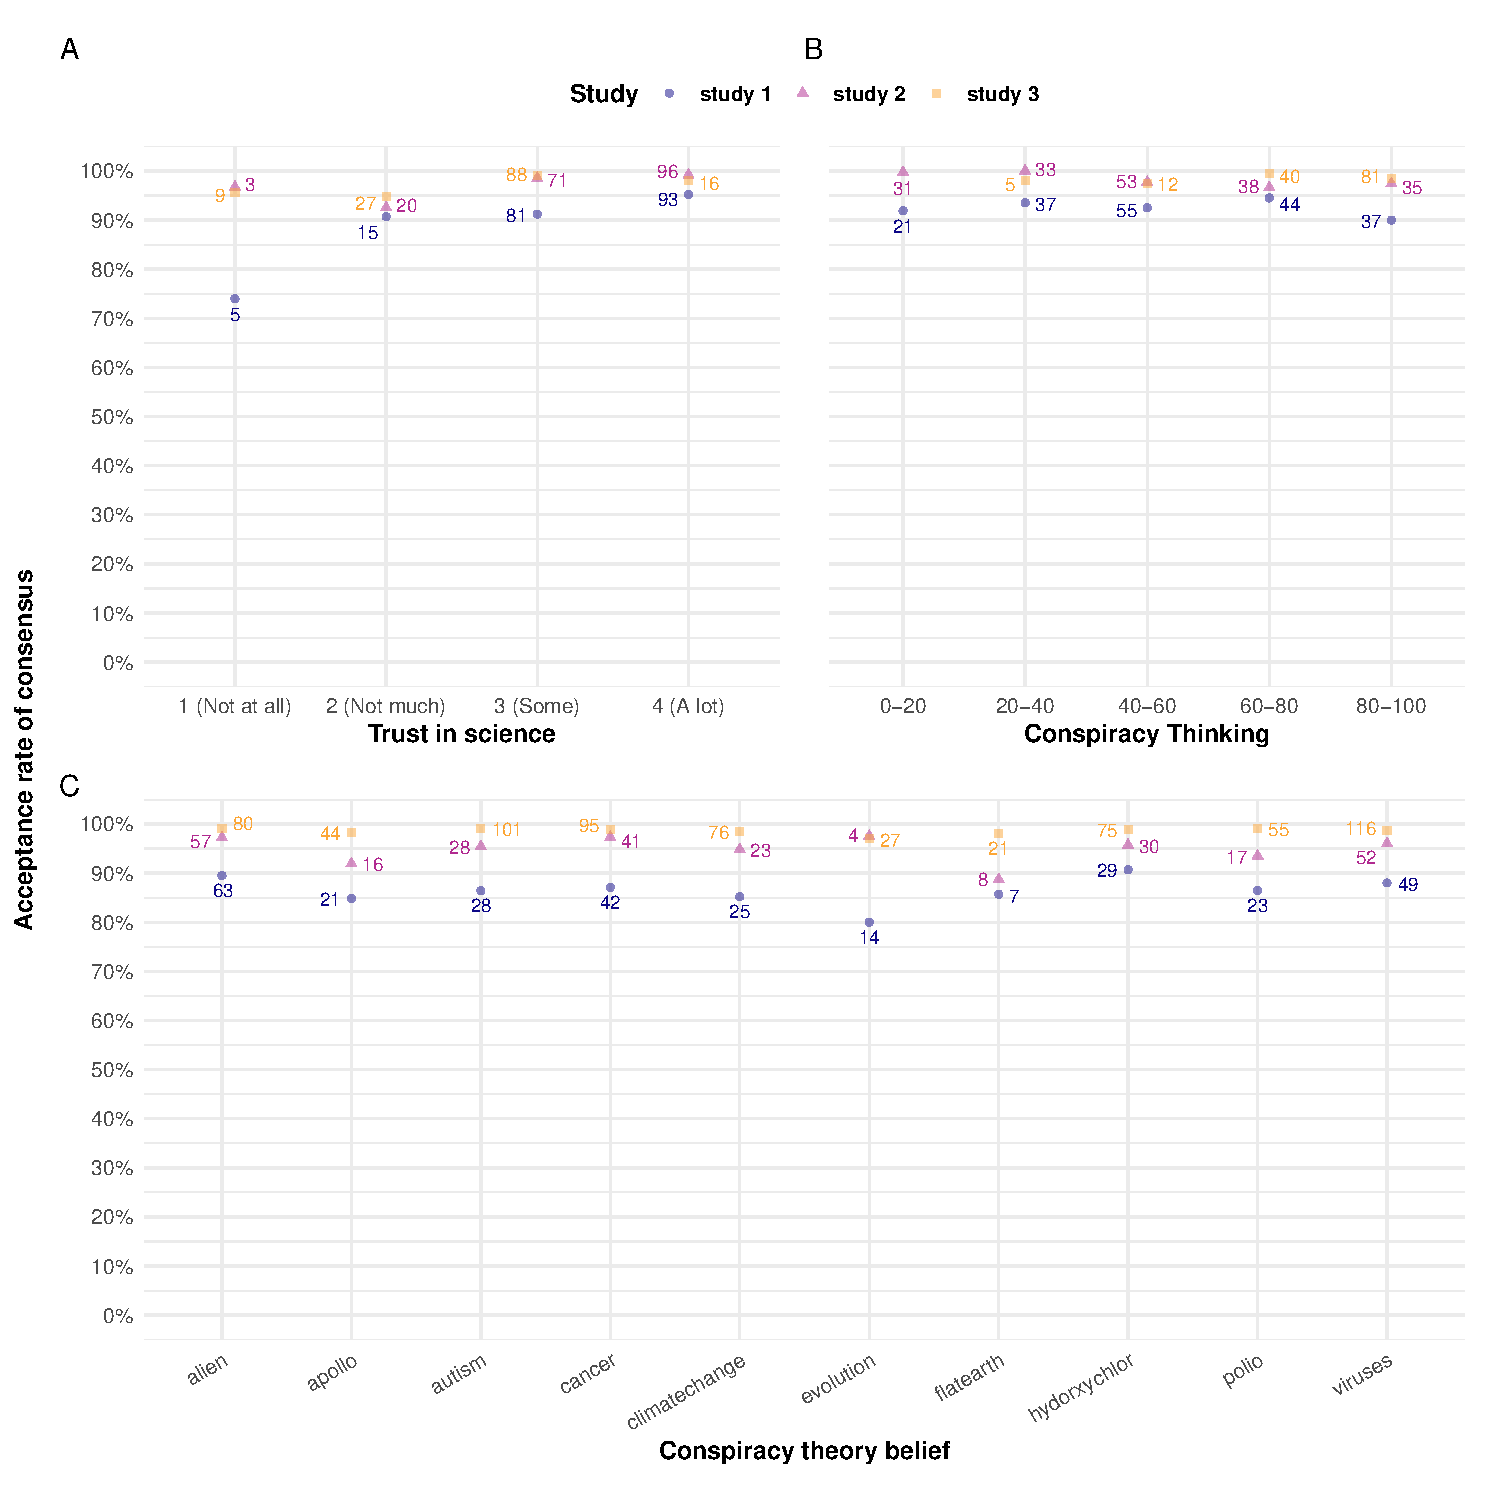
\includegraphics{output/figures/summary-plot.pdf}
\caption{\label{fig:summary-plot}Points represent the average share of acceptance and numbers the absolute count of participants as a function of: \textbf{A} the level of trust in science (``In general, would you say that you trust science a lot, some, not much, or not at all? {[}1 = Not at all, 2 = Not much, 3 = Some, 4 = A lot{]}''); \textbf{B} the average conspiracy thinking (CMQ, five items on a scale from 0 to 100); \textbf{C} the belief in specific conspiracy theories (i.e.~participants who answered 9, ``completely true'', for a given theory, see Table \ref{tab:conspiracy} for the list of the theories).}
\end{figure}

The main outcome of interest is acceptance of the scientifically consensual facts presented. Overall, acceptance was very high (aggregating across all studies: 95.1 \%; Study 1: 93 \%; Study 2: 98 \%; Study 3: 98 \%; Study 4: 91 \%). Note that this includes both participants who had previously correctly answered the knowledge question, and participants who changed their mind when presented with the scientific consensus. In Studies 3 and 4, we gave participants a second chance in case they had initially rejected the consensus, which slightly increased acceptance rates in those studies (initial acceptance in Study 3: 96 \%; in Study 4: 86 \%).

As shown in Figure \ref{fig:summary-plot}, these very high rates of acceptance hold for: participants who do not trust science at all (4.2 \% of participants, acceptance rate of 87.3 \%), participants who rank in the top two deciles of the conspiracy thinking scale (34.3 \% of participants, acceptance rate of 93.2 \%), participants who consider as ``completely true'' (the maximum of the 9-point scale) conspiracy theories stating that the earth is flat (3.7 \% of participants, acceptance rate of 87.2 \%), or that climate change due to fossil emissions is a hoax (11.4 \% of participants, acceptance rate of 91.7 \%).

Participants in the lowest decile of acceptance still had an average acceptance rate of 67.4 \%. Even participants who considered as ``completely true'' that the earth is flat and who said they do ``not trust science at all'' (N = 3) had an average acceptance rate of 86.7 \%.

These high acceptance rates do not merely reflect science knowledge: participants only correctly answered 65.8 \% of the questions (Study 1: 74 \%; Study 2: 79 \%; Study 3: 75 \%; Study 4: 36 \%) before they were provided with the scientifically consensual answer. Even the lowest decile in science knowledge which, on average, answered correctly only on 20 \% of the questions, had an average acceptance rate of 91.7 \%.

Did participants who had initially provided a wrong answer change their minds towards the scientific consensus? Yes. In most cases (study 1: 76.3 \%; study 2: 92.9 \%; study 3: 95.5 \%; study 4: 89.5 \%), participants readily accepted the scientific consensus after having initially given the wrong answer to a question.

Regarding H1, we find a consistent association between trust in science and acceptance of the scientific consensus (Studies 1: r = 0.27, p \textless{} .001; 2: r = 0.30, p \textless{} .001; 3: r = 0.20, p = 0.019; 4: r = 0.16, p = 0.029), but a less consistent relation between trust in science and science knowledge (Studies 1: r = 0.29, p \textless{} .001; 2: r = 0.28, p \textless{} .001; 3: r = 0.14, p = 0.100; 4: r = 0.10, p = 0.144).

Regarding H2, the results are mixed for the relation of conspiracy beliefs (measured as the average acceptance of all the conspiracy beliefs) with both acceptance of the scientific consensus (Studies 1: r = -0.33, p \textless{} .001; 2: r = -0.37, p \textless{} .001; 3: r = -0.02, p = 0.788; 4: r = -0.05, p = 0.498) and science knowledge (Studies 1: r = -0.38, p \textless{} .001; 2: r = -0.40, p \textless{} .001; 3: r = -0.16, p = 0.055; 4: r = -0.02, p = 0.742).

Why did participants reject the scientific consensus? We collected a total of 364 answers (study 2: 35; study 3: 74; study 4: 255) from 167 (study 2: 25; study 3: 47; study 4: 95) different participants to the open-ended questions on why they had rejected the scientific consensus on a particular question. Based on the answers, we created five categories. Table \ref{tab:justifications} summarizes these answers by five categories. All answers can be read in the ESM.

\begin{table}[tbp]

\begin{center}
\begin{threeparttable}

\caption{\label{tab:justifications}Justifications by category for data from studies 2, 3 and 4 combined.}

\begin{tabular}{llll}
\toprule
Category & \multicolumn{1}{c}{N (instances)} & \multicolumn{1}{c}{Share (instances)} & \multicolumn{1}{c}{N (unique participants)}\\
\midrule
Not convinced & 158 & 43.4\% & 70\\
No justification & 103 & 28.3\% & 51\\
Personal convictions & 43 & 11.8\% & 31\\
Mistake & 42 & 11.5\% & 34\\
Religious Beliefs & 18 & 4.9\% & 13\\
\bottomrule
\end{tabular}

\end{threeparttable}
\end{center}

\end{table}

Why did participants accept the scientific consensus? In Studies 3 and 4--the vaccine hesitant samples--we had asked participants about cases in which they agreed with the scientific consensus. A total of 320 (Study 3: 122; Study 4: 198) participants answered this question. There were more participants saying they accepted the scientific consensus because they independently verified the fact (Study 3: 47.5\%; Study 4: 47\% ), than participants saying it was because they trust scientists (Study 3: 41.8\%; Study 4: 36.4\%)\footnote{10.7\% in Study 3 and 16.7\% in Study 4 answered with ``other'' and gave an open-ended explanation (see ESM).}. We asked participants who said they verified independently to explain how they did it (answers can be found in the ESM).

In an exploratory analysis, we ran linear regressions to test whether there are differences between participants who said they had trusted science and those who said they had verified the information independently. Perhaps unsurprisingly, those who said they accepted consensus because of trust in scientists reported to trust science more (Study 3: mean = 3; \(\hat{\beta}_{\text{Trust}}\) = 0.19, p = 0.330 on a scale from 1 to 4; Study 4: mean = 2.92; \(\hat{\beta}_{\text{Trust}}\) = 0.46, p \textless{} .001) than those who said they verified independently (Study 3 mean = 2.81; Study 4 mean = 2.45). We did not find a difference regarding acceptance (Study 3: \(\hat{\beta}_{\text{Acceptance}}\) = 0.01, p = 0.523 on a scale from 0 to 1; Study 4: \(\hat{\beta}_{\text{Acceptance}}\) = 0.04, p = 0.116) or regarding beliefs in conspiracy theories (Study 3: \(\hat{\beta}_{\text{BCTI}}\) = -0.16, p = 0.694 on a scale from 1 to 9; Study 4: \(\hat{\beta}_{\text{BCTI}}\) = -0.21, p = 0.322). We also did not find a difference in time spent on the survey in Study 3 (\(\hat{\beta}_{\text{Time}}\) = -0.02, p = 0.985; median = 7.64 mins), but in Study 4, people who said they had accepted the consensus because they they trust scientists tended to spend on average 2 minutes less on the survey (\(\hat{\beta}_{\text{Time}}\) = -2.16, p = 0.018; median = 9.38 mins).\footnote{For these analyses, we excluded outliers who took over 30mins for the survey, which was estimated to take around 10 mins, and for which the median time was 7 minutes. As a result, we excluded 1 participant in Study 3 and 4 in Study 4. Significance levels remain the same when including these outliers.} In Study 4, in which we used facts that participants were unlikely to have encountered before, we tracked whether people clicked on the source links we provided--a behavior that you would expect from people who report verifying facts independently. On average, participants clicked only on 1.36 links (out of 20 possible clicks) and there was no difference between the two groups (\(\hat{\beta}_{\text{Clicks}}\) = -1.09, p = 0.062).

More detailed results addressing all our pre-registered research questions can be found in the ESM.

\section{Discussion}\label{discussion}

US participants were asked whether they accepted scientifically consensual answers on basic science questions.We found quasi-universal acceptance of basic science, with an overall rate of acceptance of 95.1 \%, which remained very high for participants who declared not trusting science at all (87.3 \% of acceptance), or who endorsed theories blatantly violating scientific knowledge, such as flat earth (87.2 \% of acceptance).

Overall, the present findings support the motivated rejection of science model (Lewandowsky \& Oberauer, 2016), in which ``people tend to reject findings that threaten their core beliefs or worldview'' (p.~217). A number of participants in our studies rejected basic tenets of science (on evolution, the shape of the earth, etc.). However, they still accepted the vast majority of basic scientific knowledge presented to them. This suggests that these participants had reasons to reject specific scientific knowledge, and that this rejection prompted them to express a lower trust in science when asked general questions on the topic. These participants did not appear to have general grounds for distrusting science, which should have led them to reject most or all of the science knowledge presented to them.

Our findings are also relevant for the knowledge--attitudes model of trust in science (see, e.g., Bauer, Allum, \& Miller, 2007). The fact that even people with low science knowledge trust most of basic science might be taken as showing the power of even a modicum of science knowledge; on the other hand, it also means that attempts at increasing science knowledge in general might not have much effect on trust in science, by contrast with targeting the specific beliefs people are motivated to reject.

Finally, some of the present results also speak to the alienation model (Gauchat, 2011), and more specifically to the need for epistemic autonomy (Fricker, 2006). Declaring not trusting science, or endorsing conspiracy theories (Harris, 2023) might reflect a desire to maintain epistemic autonomy and not appear to `blindly' accept epistemic authority. The acceptance of basic science facts would be reconciled with this need to appear epistemically autonomous by the suggestion that the acceptance stems from independent evaluation instead of trust (however implausible that might be: it's not clear how participants could independently verify the ratio of glial cells to neurons, say, and few participants appeared to have engaged in even simple forms of verification).

In applied terms, the present results suggest the existence of a vast reservoir of trust in basic science that could be tapped into in science communication. Since people appear so resistant to rejecting basic science, stressing the basic science components of publicly controversial fields, from GMOs to climate change, might help reduce the `consensus gaps' observed in these domains (on climate change, see, e.g. Ranney \& Clark, 2016).

The present studies have a number of limitations, in particular the lack of representative samples, and the focus on a single country. We hope that future studies will extend our findings to other populations.

\FloatBarrier

\section{References}\label{references}

\phantomsection\label{refs}
\begin{CSLReferences}{1}{0}
\bibitem[\citeproctext]{ref-alganTrustScientistsTimes2021}
Algan, Y., Cohen, D., Davoine, E., Foucault, M., \& Stantcheva, S. (2021). Trust in scientists in times of pandemic: Panel evidence from 12 countries. \emph{Proceedings of the National Academy of Sciences}, \emph{118}(40), e2108576118. \url{https://doi.org/10.1073/pnas.2108576118}

\bibitem[\citeproctext]{ref-allumScienceKnowledgeAttitudes2008}
Allum, N., Sturgis, P., Tabourazi, D., \& Brunton-Smith, I. (2008). Science knowledge and attitudes across cultures: a meta-analysis. \emph{Public Understanding of Science}, \emph{17}(1), 35--54. \url{https://doi.org/10.1177/0963662506070159}

\bibitem[\citeproctext]{ref-bauerWhatCanWe2007}
Bauer, M. W., Allum, N., \& Miller, S. (2007). What can we learn from 25 years of PUS survey research? Liberating and expanding the agenda. \emph{Public Understanding of Science}, \emph{16}(1), 79--95. \url{https://doi.org/10.1177/0963662506071287}

\bibitem[\citeproctext]{ref-brianAmericansTrustScientists2023}
Brian, K., \& Tyson, A. (2023). \emph{Americans{'} trust in scientists, positive views of science continue to decline}. Retrieved from \url{https://www.pewresearch.org/science/2023/11/14/americans-trust-in-scientists-positive-views-of-science-continue-to-decline/}

\bibitem[\citeproctext]{ref-bruderMeasuringIndividualDifferences2013}
Bruder, M., Haffke, P., Neave, N., Nouripanah, N., \& Imhoff, R. (2013). Measuring individual differences in generic beliefs in conspiracy theories across cultures: Conspiracy mentality questionnaire. \emph{Frontiers in Psychology}, \emph{4}. Retrieved from \url{https://www.frontiersin.org/articles/10.3389/fpsyg.2013.00225}

\bibitem[\citeproctext]{ref-colognaTrustScientistsTheir2024}
Cologna, V., Mede, N. G., Berger, S., Besley, J., Brick, C., Joubert, M., \ldots{} Linden, D. S. van der. (2024). \emph{Trust in scientists and their role in society across 67 countries}. \url{https://doi.org/10.31219/osf.io/6ay7s}

\bibitem[\citeproctext]{ref-colognaRoleTrustClimate2020}
Cologna, V., \& Siegrist, M. (2020). The role of trust for climate change mitigation and adaptation behaviour: A meta-analysis. \emph{Journal of Environmental Psychology}, \emph{69}, 101428. \url{https://doi.org/10.1016/j.jenvp.2020.101428}

\bibitem[\citeproctext]{ref-durantPublicUnderstandingScience1989}
Durant, J. R., Evans, G. A., \& Thomas, G. P. (1989). The public understanding of science. \emph{Nature}, \emph{340}(6228), 11--14. \url{https://doi.org/10.1038/340011a0}

\bibitem[\citeproctext]{ref-frickerTestimonyEpistemicAutonomy2006}
Fricker, E. (2006). \emph{Testimony and Epistemic Autonomy} (J. Lackey \& E. Sosa, Eds.). Oxford University PressOxford. \url{https://doi.org/10.1093/acprof:oso/9780199276011.003.0011}

\bibitem[\citeproctext]{ref-funkKeyFindingsPublic2019}
Funk, C., Johnson, C., \& Hefferon, M. (2019). \emph{5 key findings about public trust in scientists in the u.s.} Retrieved from \url{https://www.pewresearch.org/fact-tank/2019/08/05/5-key-findings-about-public-trust-in-scientists-in-the-u-s/}

\bibitem[\citeproctext]{ref-gauchatCulturalAuthorityScience2011}
Gauchat, G. (2011). The cultural authority of science: Public trust and acceptance of organized science. \emph{Public Understanding of Science}, \emph{20}(6), 751--770. \url{https://doi.org/10.1177/0963662510365246}

\bibitem[\citeproctext]{ref-gauchatPoliticizationSciencePublic2012}
Gauchat, G. (2012). Politicization of Science in the Public Sphere: A Study of Public Trust in the United States, 1974 to 2010. \emph{American Sociological Review}, \emph{77}(2), 167--187. \url{https://doi.org/10.1177/0003122412438225}

\bibitem[\citeproctext]{ref-harrisConspiracyTheoriesPopulism2023}
Harris, K. R. (2023). Conspiracy Theories, Populism, and Epistemic Autonomy. \emph{Journal of the American Philosophical Association}, \emph{9}(1), 21--36. \url{https://doi.org/10.1017/apa.2021.44}

\bibitem[\citeproctext]{ref-krauseTrendsAmericansTrust2019a}
Krause, N. M., Brossard, D., Scheufele, D. A., Xenos, M. A., \& Franke, K. (2019). Trends{\textemdash}americans{'} trust in science and scientists. \emph{Public Opinion Quarterly}, \emph{83}(4), 817--836. \url{https://doi.org/10.1093/poq/nfz041}

\bibitem[\citeproctext]{ref-lantianMeasuringBeliefConspiracy2016}
Lantian, A., Muller, D., Nurra, C., \& Douglas, K. M. (2016). Measuring Belief in Conspiracy Theories: Validation of a French and English Single-Item Scale. \emph{International Review of Social Psychology}, \emph{29}(1), 1. \url{https://doi.org/10.5334/irsp.8}

\bibitem[\citeproctext]{ref-lewandowskyMotivatedRejectionScience2016}
Lewandowsky, S., \& Oberauer, K. (2016). Motivated Rejection of Science. \emph{Current Directions in Psychological Science}, \emph{25}(4), 217--222. \url{https://doi.org/10.1177/0963721416654436}

\bibitem[\citeproctext]{ref-liPolarizationPublicTrust2022}
Li, N., \& Qian, Y. (2022). Polarization of public trust in scientists between 1978 and 2018: Insights from a cross-decade comparison using interpretable machine learning. \emph{Politics and the Life Sciences}, \emph{41}(1), 45--54. \url{https://doi.org/10.1017/pls.2021.18}

\bibitem[\citeproctext]{ref-lindholtPublicAcceptanceCOVID192021}
Lindholt, M. F., Jørgensen, F., Bor, A., \& Petersen, M. B. (2021). Public acceptance of COVID-19 vaccines: cross-national evidence on levels and individual-level predictors using observational data. \emph{BMJ Open}, \emph{11}(6), e048172. \url{https://doi.org/10.1136/bmjopen-2020-048172}

\bibitem[\citeproctext]{ref-millerMeasurementCivicScientific1998a}
Miller, J. D. (1998). The measurement of civic scientific literacy. \emph{Public Understanding of Science}, \emph{7}(3), 203--223. \url{https://doi.org/10.1088/0963-6625/7/3/001}

\bibitem[\citeproctext]{ref-pennycookOverconfidentlyConspiratorialConspiracy2022}
Pennycook, G., Binnendyk, J., \& Rand, D. (2022). \emph{Overconfidently conspiratorial: Conspiracy believers are dispositionally overconfident and massively overestimate how much others agree with them}. \url{https://doi.org/10.31234/osf.io/d5fz2}

\bibitem[\citeproctext]{ref-ranneyClimateChangeConceptual2016}
Ranney, M. A., \& Clark, D. (2016). Climate Change Conceptual Change: Scientific Information Can Transform Attitudes. \emph{Topics in Cognitive Science}, \emph{8}(1), 49--75. \url{https://doi.org/10.1111/tops.12187}

\bibitem[\citeproctext]{ref-committeeonscienceliteracyandpublicperceptionofscienceScienceLiteracyConcepts2016}
Science Literacy, C. on, Public Perception of Science, Board on Science Education, Behavioral, D. of, Sciences, S., Education, \& National Academies of Sciences, Engineering, and Medicine. (2016). \emph{Science Literacy: Concepts, Contexts, and Consequences} (C. E. Snow \& K. A. Dibner, Eds.). Washington, D.C.: National Academies Press. \url{https://doi.org/10.17226/23595}

\bibitem[\citeproctext]{ref-sturgisTrustScienceSocial2021}
Sturgis, P., Brunton-Smith, I., \& Jackson, J. (2021). Trust in science, social consensus and vaccine confidence. \emph{Nature Human Behaviour}, \emph{5}(11), 1528--1534. \url{https://doi.org/10.1038/s41562-021-01115-7}

\bibitem[\citeproctext]{ref-vanstekelenburgScientificConsensusCommunicationContested2022}
Van Stekelenburg, A., Schaap, G., Veling, H., Van 'T Riet, J., \& Buijzen, M. (2022). Scientific-Consensus Communication About Contested Science: A Preregistered Meta-Analysis. \emph{Psychological Science}, \emph{33}(12), 1989--2008. \url{https://doi.org/10.1177/09567976221083219}

\bibitem[\citeproctext]{ref-veckalov27countryTestCommunicating2024}
Većkalov, B., Geiger, S. J., Bartoš, F., White, M. P., Rutjens, B. T., Harreveld, F. van, \ldots{} Linden, S. van der. (2024). A 27-country test of communicating the scientific consensus on climate change. \emph{Nature Human Behaviour}, 1--14. \url{https://doi.org/10.1038/s41562-024-01928-2}

\bibitem[\citeproctext]{ref-wellcomeglobalmonitorWellcomeGlobalMonitor2018}
Wellcome Global Monitor. (2018). \emph{Wellcome Global Monitor 2018}. Retrieved from \url{https://wellcome.org/reports/wellcome-global-monitor/2018}

\bibitem[\citeproctext]{ref-wellcomeglobalmonitorWellcomeGlobalMonitor2020}
Wellcome Global Monitor. (2020). \emph{Wellcome Global Monitor 2020: Covid-19}. Retrieved from \url{https://wellcome.org/reports/wellcome-global-monitor-covid-19/2020}

\bibitem[\citeproctext]{ref-wellcomeglobalmonitorPublicTrustScientists2021}
Wellcome Global Monitor. (2021). \emph{Public trust in scientists rose during the Covid-19 pandemic \textbar{} News}. Retrieved from \url{https://wellcome.org/news/public-trust-scientists-rose-during-covid-19-pandemic}

\end{CSLReferences}

\newpage

\appendix


\section{Acceptance conditional on knowledge}\label{acceptance-knowledge}

Did participants who had initially gotten it wrong change their minds towards the scientific consensus? Yes. In most cases (study 1: 76.3 \%; study 2: 92.9 \%; study 3: 95.5 \%; study 4: 89.5 \%), participants readily accepted the scientific consensus after having initially given the wrong answer to a question. In very few cases, participants changed their mind away from the scientific consensus. These participants initially gave the correct response, but rejected the scientific consensus right after, thereby contradicting their own initial response (study 1: 1.6 \%; study 2: 0.5 \%; study 3: 0.7 \%; study 4: 5.7 \%). Figure \ref{fig:acceptance-knowledge} shows acceptance rates conditional on whether the initial answer to the questions was correct or not.



\begin{figure}
\centering
\includegraphics{output/figures/acceptance-knowledge.pdf}
\caption{\label{fig:acceptance-knowledge}Acceptance rates of scientific consensus, based on whether the initial response to the knowledge question was false or true.}
\end{figure}

\clearpage

\section{Experiment 1}\label{exp1}

\subsection{Participants}\label{participants-1}

We recruited 200 participants from the US via prolific. 6 participants failed our attention check, resulting in a final sample of 194 participants (98 female, 96 male; \(age_\text{mean}\): 41.71, \(age_\text{sd}\): 13.07, \(age_\text{median}\): 39). Since we did not have any prior assumptions on effect sizes, we did not do a power analysis.

\subsection{Materials}\label{materials-2}

\FloatBarrier



\begin{figure}

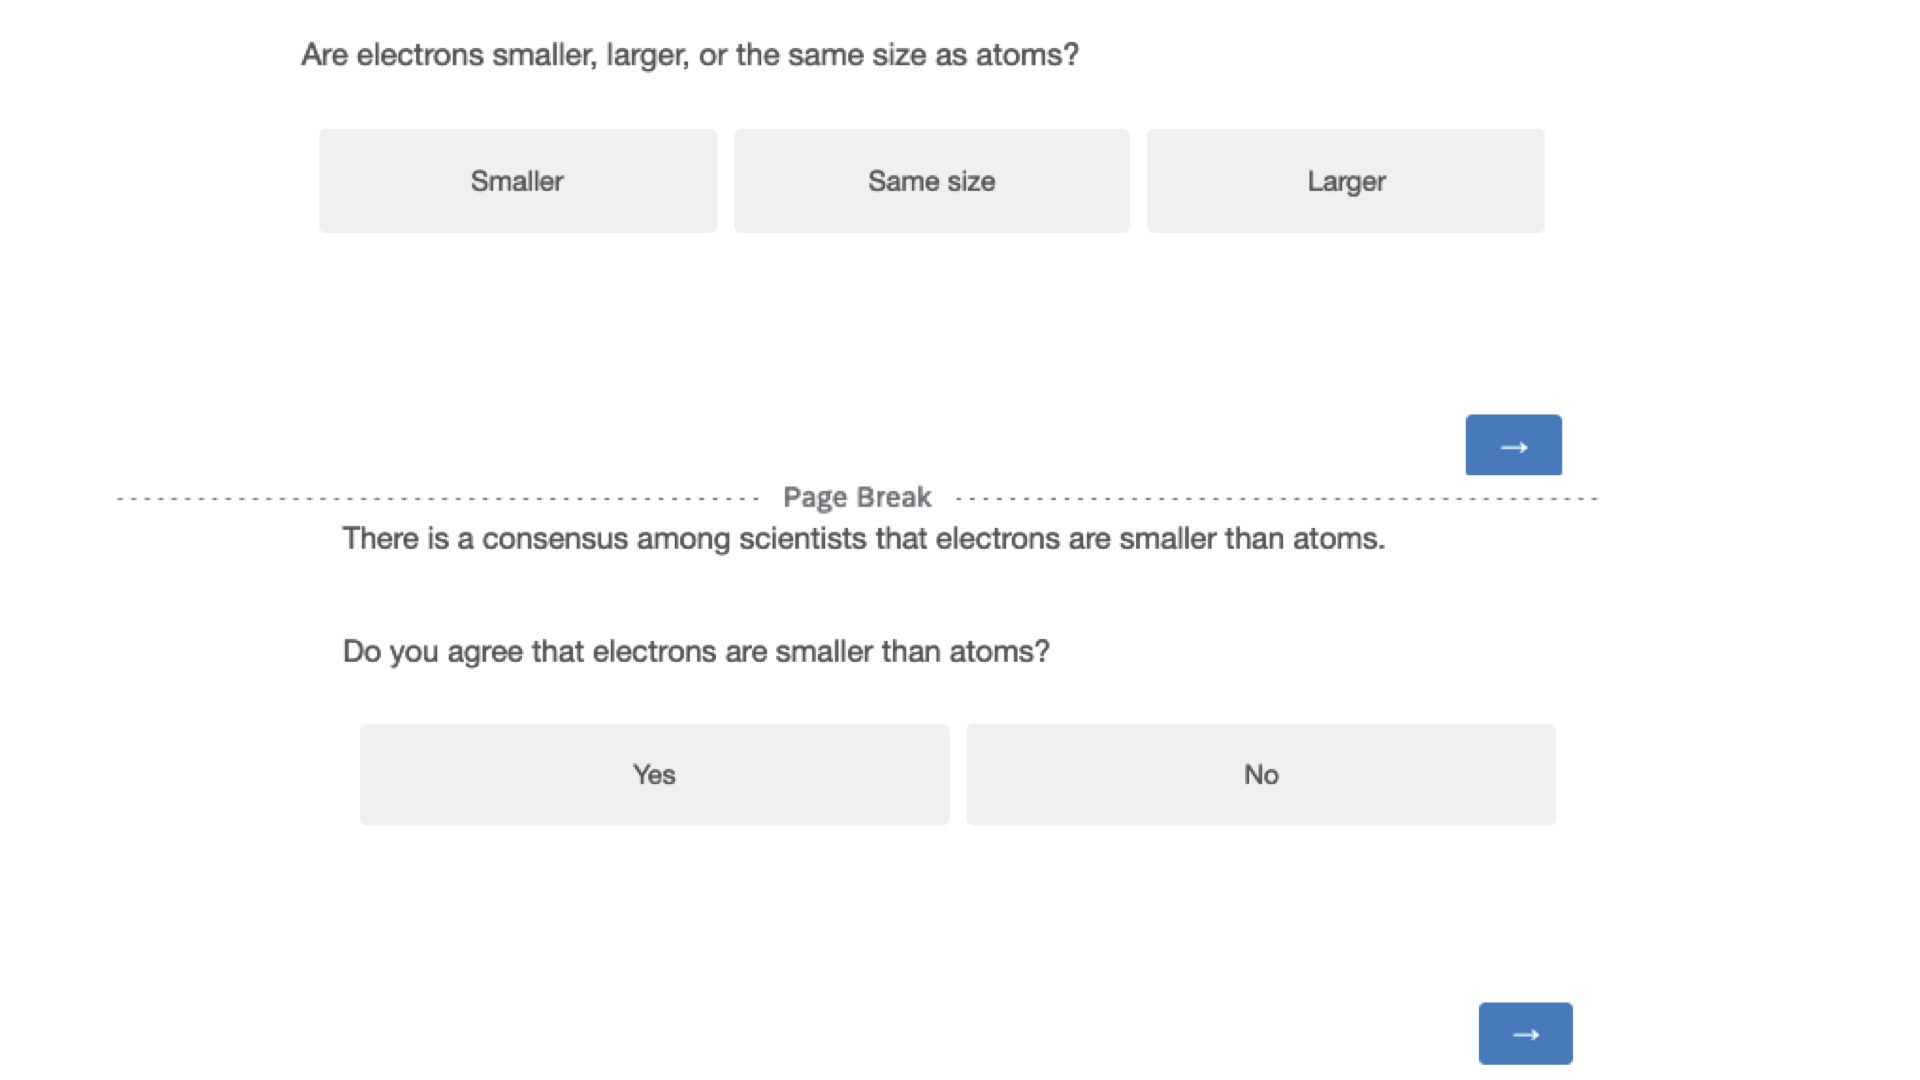
\includegraphics[width=1\linewidth]{./figures/study1_question_example} \hfill{}

\caption{Example of a science question, the scientific consensus and the corresponding acceptance question.}\label{fig:stimulus-example}
\end{figure}

\subsubsection{Conspiracy scales}\label{conspiracy-scales}

Beside Belief in Conspiracy Theory Inventory (BCTI) by Pennycook et al. (2022) which report in the main study, we also assessed two other consipiracy thinking measures:

\begin{enumerate}
\def\labelenumi{\arabic{enumi}.}
\tightlist
\item
  The conspiracy mentality questionnaire (CMQ) by Bruder et al. (2013):
  I think that . . .
\end{enumerate}

\begin{itemize}
\tightlist
\item
  \ldots{} many very important things happen in the world, which the public is never informed about. - politicians usually do not tell us the true motives for their decisions.
\item
  \ldots{} government agencies closely monitor all citizens.
\item
  \ldots{} events which superficially seem to lack a connection are often the result of secret activities.
\item
  \ldots{} there are secret organizations that greatly influence political decisions.
\end{itemize}

{[}0\% - 100\%; 0 = certainly not, 100 = certain{]}

\begin{enumerate}
\def\labelenumi{\arabic{enumi}.}
\setcounter{enumi}{1}
\tightlist
\item
  The Single Item Conspiracy Beliefs Scale (SICBS) by Lantian et al. (2016) :
\end{enumerate}

\begin{itemize}
\tightlist
\item
  I think that the official version of the events given by the authorities very often hides the truth. {[}1-9; 1 = Completely false, 5 = Unsure, 9 = Completely true{]}
\end{itemize}

\subsubsection{Trust in science}\label{trust-in-science-1}

We rely on three items

\begin{enumerate}
\def\labelenumi{\arabic{enumi}.}
\item
  How much do you trust scientists in this country? Do you trust them a lot, some, not much, or not at all? {[}1 = Not at all, 2 = Not much, 3 = Some, 4 = A lot{]}
\item
  In general, would you say that you trust science a lot, some, not much, or not at all? {[}1 = Not at all, 2 = Not much, 3 = Some, 4 = A lot{]}
\item
  How much confidence do you have in scientists to act in the best interests of the public? {[}1-5; 1 = No confidence at all, 5 = A great deal of confidence{]}
\end{enumerate}

\subsection{Results}\label{results-1}

Regarding RQ1 and RQ2, participants answered on average 74 \% (sd = 0.16) of the questions correctly, and accepted the scientific consensus on average for 93 \% (sd = 0.12) of the questions.

Fig. \ref{fig:exp1-conditional-acceptance} illustrates the relationship between knowledge and acceptance. In most cases (76.3 \%), participants readily accepted the scientific consensus after having given the wrong answer to a question. In very few cases (1.6 \%), participants who gave the correct response afterwards rejected the scientific consensus, thereby contradicting their own initial response. We believe this might have been due to inattention.

For RQ3, we find a positive but small correlation between both science knowledge and trust in science (r = 0.29, p \textless{} .001), and acceptance of scientific consensus and trust in science (r = 0.27, p \textless{} .001). The more people are knowledgeable about science and the more they tend to accept the scientific consensus, the more they tend to trust science. These correlations are relatively weak, which might be partly due to ceiling effects: As illustrated in Fig. \ref{fig:exp1-plot}, (i) most people do trust science, and (ii) that is true even among people with low knowledge or acceptance rates.

For RQ4, we find a negative correlation of similar magnitude between conspiracy thinking and science knowledge (r = -0.38, p \textless{} .001), and conspiracy thinking and acceptance of scientific consensus (r = -0.33, p \textless{} .001).

In Appendix \ref{exp1}, we show that these associations are robust when using alternative measures of trust and conspiracy thinking. Appendix \ref{exp1} also includes more descriptive statistics, such as knowledge and acceptance by science questions.

Are trust in science and conspiracy thinking, respectively, associated with being more easily convinced of the scientific consensus? In our main analyses, we looked at correlations of acceptance across all observations. One possibility is that the associations between trust in science/conspiracy thinking and acceptance of scientific consensus are explained by science knowledge: People who give the right answer in the first place are more ready to accept the consensus, and trust in science/conspiracy thinking are mostly associated with this knowledge, but not with willingness to accept the consensus. To addressed this potential confound, in a non-preregistered analysis, we restricted our sample to cases where participants gave the wrong answer to the knowledge question. We then calculated the correlation between trust in science and average acceptance rate by participant. We find no statistically significant correlation of acceptance with neither conspiracy thinking (r = -0.14, p = 0.061), nor with trust in science (r = 0.06, p = 0.387).

\subsection{Discussion}\label{discussion-1}

These results suggest that most people accept the scientific consensus most of the time. Even when people do not know the correct answer to a science question, they tend to mostly accept the scientific consensus afterwards. Yet, in 23.7 \% of the cases, participants rejected the scientific consensus after having given the wrong answer, suggesting that simply stating the consensus is not sufficient to convince participants sometimes. In general, people with lower trust in science and who believe more in conspiracy theories tend to both know less about science and accept the scientific consensus less.

\subsection{Comparing items}\label{comparing-items}

\subsubsection{Conspiracy theories}\label{conspiracy-theories}

Table \ref{tab:correlation-conspiracy} shows the correlations of the three different scales assessing conspiracy thinking.

\begin{table}[h]

\begin{center}
\begin{threeparttable}

\caption{\label{tab:correlation-conspiracy}Correlations of the three different scales assessing conspiracy thinking}

\begin{tabular}{llll}
\toprule
 & \multicolumn{1}{c}{BCTI} & \multicolumn{1}{c}{CMQ} & \multicolumn{1}{c}{SICBS}\\
\midrule
BCTI & 1.00 & 0.58 & 0.56\\
CMQ & 0.58 & 1.00 & 0.77\\
SICBS & 0.56 & 0.77 & 1.00\\
\bottomrule
\end{tabular}

\end{threeparttable}
\end{center}

\end{table}

\subsubsection{Trust in science}\label{trust-in-science-2}

Table \ref{tab:correlation-trust} shows the correlations of the three different items measuring trust in science.

\begin{table}[h]

\begin{center}
\begin{threeparttable}

\caption{\label{tab:correlation-trust}Correlations of the three different items measuring trust in science}

\begin{tabular}{llll}
\toprule
 & \multicolumn{1}{c}{wgm\_sciencegeneral} & \multicolumn{1}{c}{wgm\_scientists} & \multicolumn{1}{c}{pew}\\
\midrule
wgm\_sciencegeneral & 1.00 & 0.85 & 0.75\\
wgm\_scientists & 0.85 & 1.00 & 0.82\\
pew & 0.75 & 0.82 & 1.00\\
\bottomrule
\end{tabular}

\end{threeparttable}
\end{center}

\end{table}

\subsection{Correlations with alternative measures}\label{correlations-with-alternative-measures}

Table \ref{tab:correlations-outcomes} shows the correlations between knowledge and acceptance, respectively, and outcome variables.

\begin{table}[tbp]

\begin{center}
\begin{threeparttable}

\caption{\label{tab:correlations-outcomes}Correlations between knowledge and acceptance, respectively, and outcome variables}

\begin{tabular}{lll}
\toprule
outcome & \multicolumn{1}{c}{Correlation with knowledge} & \multicolumn{1}{c}{Correlation with acceptance}\\
\midrule
BCTI 
(main conspiracy measure) & -0.38 (p< .001) & -0.33 (p< .001)\\
CMQ & -0.11 (p= 0.121) & -0.07 (p= 0.317)\\
SICBS & -0.1 (p= 0.158) & -0.09 (p= 0.213)\\
WGM trust scientists & 0.23 (p= 0.001) & 0.26 (p< .001)\\
WGM trust general 
(main trust measure) & 0.29 (p< .001) & 0.27 (p< .001)\\
PEW trust scientists & 0.16 (p= 0.027) & 0.21 (p= 0.003)\\
\bottomrule
\end{tabular}

\end{threeparttable}
\end{center}

\end{table}

\subsection{Results conditional on false responses}\label{results-conditional-on-false-responses}

Table \ref{tab:false-response-regression} shows the correlations between acceptance and outcome variables based on linear regression models on standardized values.

\begin{table}

\caption{\label{tab:false-response-regression}Based on false response data only, correlations between acceptance and outcome variables based on linear regression models on standardized values}
\centering
\begin{tabular}[t]{lcccccc}
\toprule
  & BCTI\_avg & CMQ\_avg & SICBS & wgm\_scientists & wgm\_sciencegeneral & pew\\
\midrule
(Intercept) & 0.000 & 0.000 & 0.000 & 0.000 & 0.000 & 0.000\\
 & (0.073) & (0.074) & (0.074) & (0.073) & (0.074) & (0.074)\\
avg\_acceptance & -0.139+ & 0.008 & -0.028 & 0.108 & 0.064 & 0.056\\
 & (0.073) & (0.074) & (0.074) & (0.074) & (0.074) & (0.074)\\
\midrule
Num.Obs. & 184 & 184 & 184 & 184 & 184 & 184\\
R2 & 0.019 & 0.000 & 0.001 & 0.012 & 0.004 & 0.003\\
R2 Adj. & 0.014 & -0.005 & -0.005 & 0.006 & -0.001 & -0.002\\
AIC & 523.6 & 527.2 & 527.0 & 525.0 & 526.4 & 526.6\\
BIC & 533.2 & 536.8 & 536.7 & 534.7 & 536.1 & 536.2\\
Log.Lik. & -258.801 & -260.578 & -260.512 & -259.506 & -260.204 & -260.295\\
RMSE & 0.99 & 1.00 & 1.00 & 0.99 & 1.00 & 1.00\\
\bottomrule
\multicolumn{7}{l}{\rule{0pt}{1em}+ p $<$ 0.1, * p $<$ 0.05, ** p $<$ 0.01, *** p $<$ 0.001}\\
\end{tabular}
\end{table}

\subsection{By-question variation}\label{by-question-variation}

\subsubsection{Knowledge}\label{knowledge}



\begin{figure}
\centering
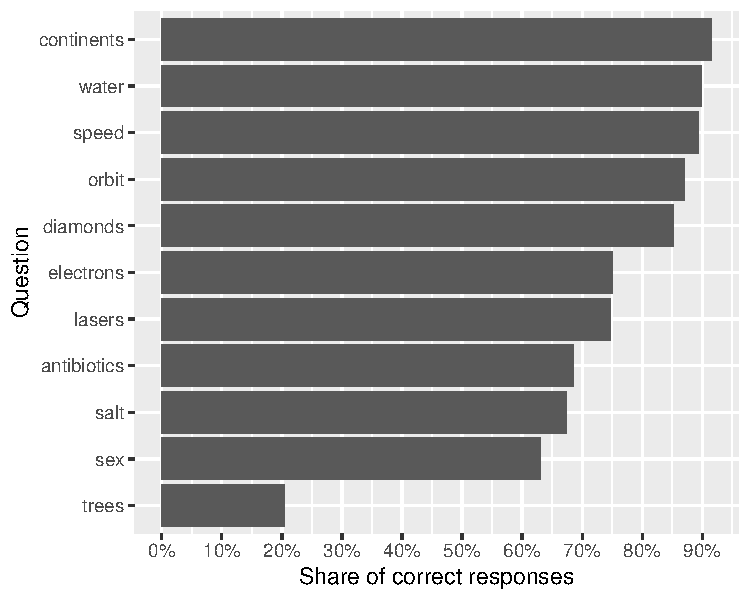
\includegraphics{output/figures/exp1-questions-knowledge.pdf}
\caption{\label{fig:exp1-questions-knowledge}Distribution of correct answers by question.}
\end{figure}

\subsubsection{Acceptance}\label{acceptance}



\begin{figure}
\centering
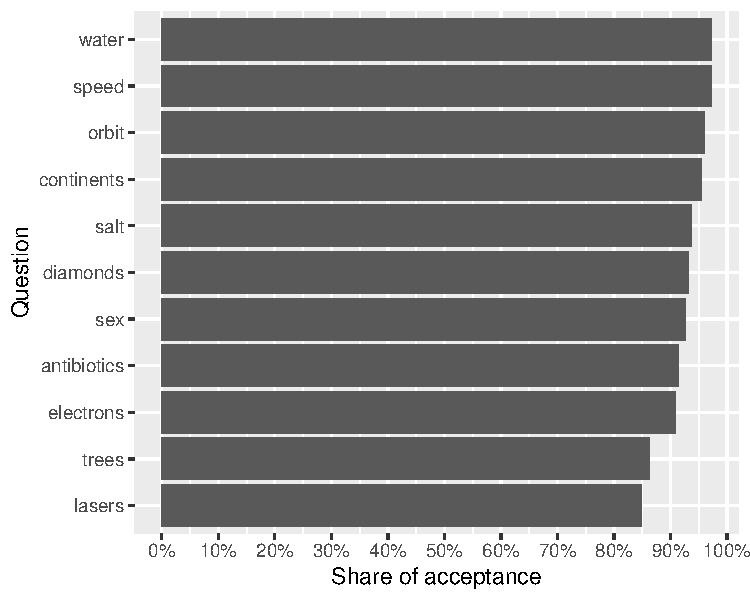
\includegraphics{output/figures/exp1-questions-acceptance.pdf}
\caption{\label{fig:exp1-questions-acceptance}Distribution of consensus acceptance by question.}
\end{figure}

\subsection{Trust in science}\label{trust-in-science-3}



\begin{figure}
\centering
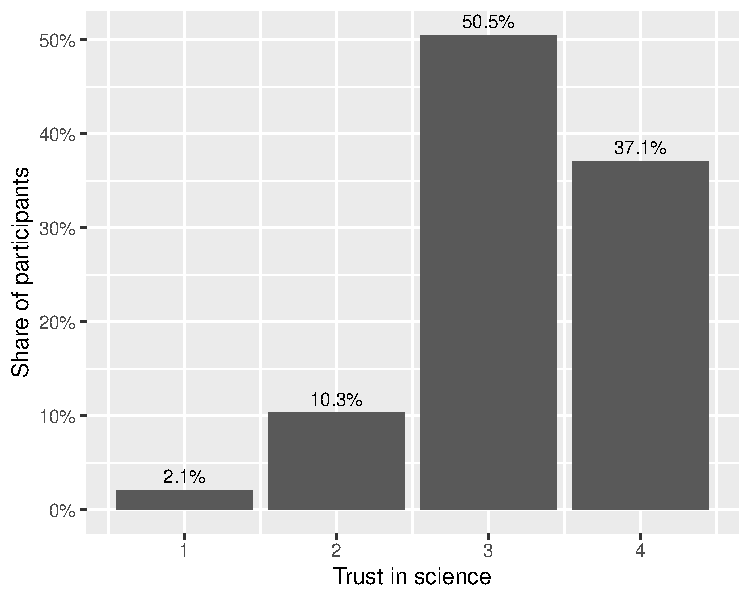
\includegraphics{output/figures/exp1-trust-scientists.pdf}
\caption{\label{fig:exp1-trust-scientists}Distribution of trust in scientists.}
\end{figure}

\subsection{Conspiracy thinking}\label{conspiracy-thinking-1}

\subsubsection{Distribution}\label{distribution}



\begin{figure}
\centering
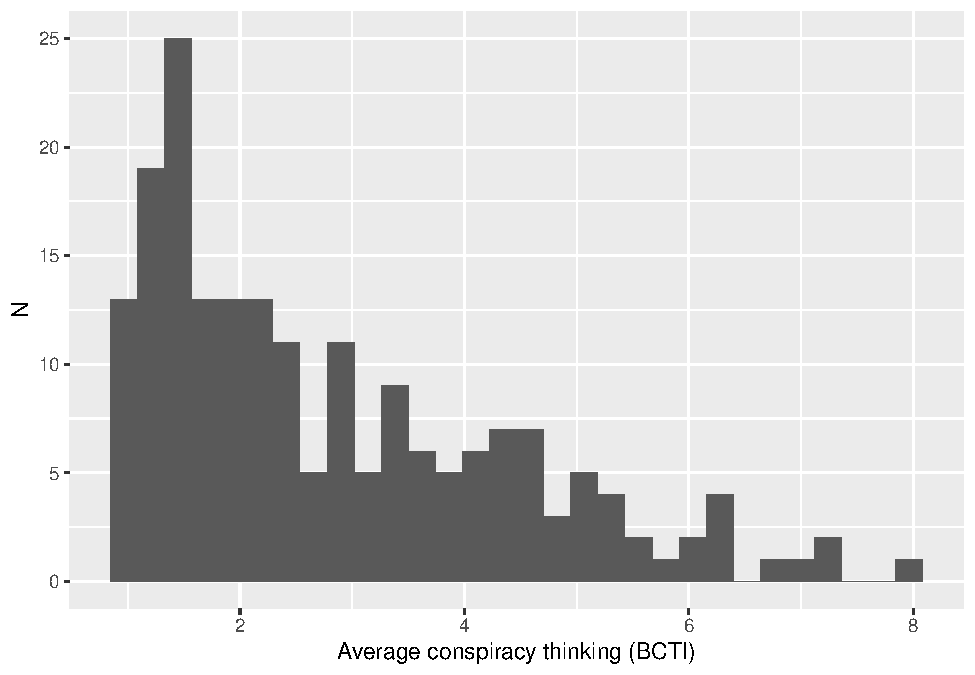
\includegraphics{output/figures/exp1-conspiracy-distribution.pdf}
\caption{\label{fig:exp1-conspiracy-distribution}Distribution of conspiracy thinking.}
\end{figure}

\subsubsection{By-item variation}\label{by-item-variation}



\begin{figure}
\centering
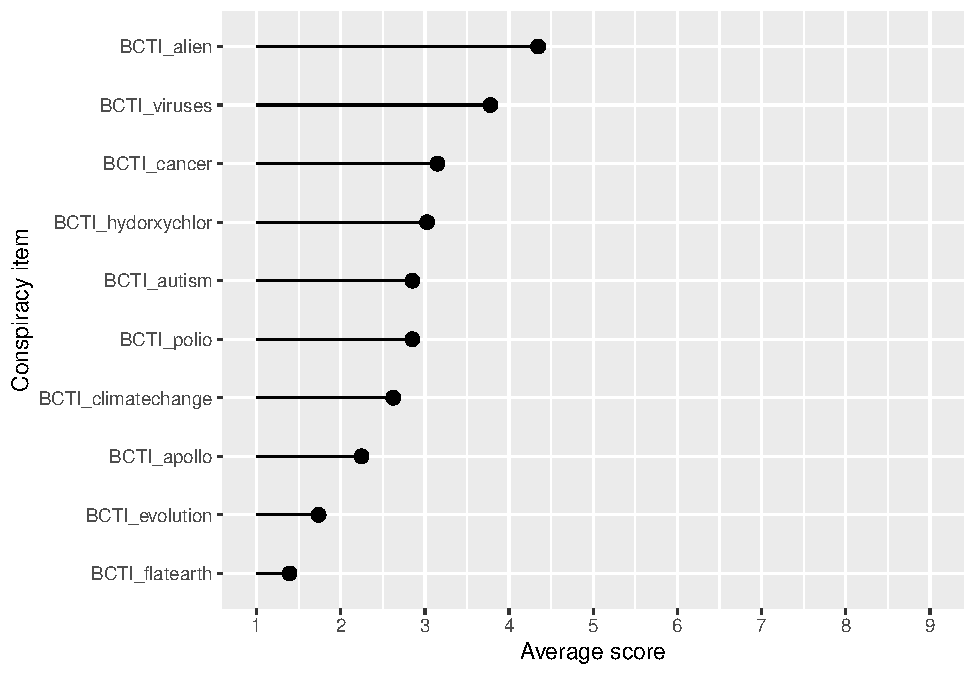
\includegraphics{output/figures/exp1-conspiracy-items.pdf}
\caption{\label{fig:exp1-conspiracy-items}Distribution of conspiracy thinking by item.}
\end{figure}

\subsection{Open ended comments}\label{open-ended-comments}

\begin{longtable}[t]{>{}r>{\raggedright\arraybackslash}p{40em}}
\caption{\label{tab:unnamed-chunk-27}Reasons for consensus rejection}\\
\toprule
id & comments\\
\midrule
1 & no\\
20 & None\\
22 & I answered thoughtfully, good luck!\\
27 & interesting, thank you.\\
30 & n/a\\
\addlinespace
32 & None\\
39 & no\\
41 & none\\
42 & n/a\\
67 & thanks\\
\addlinespace
69 & No comments\\
74 & no\\
76 & none\\
78 & None - thank you!\\
79 & Should've clicked agree about plants getting carbon from the air, but I wanted to look it up first. Whenever I encounter something I didn't know online, I like to cross-reference. In retrospect though, everything else you asked about was simple and on the level, and I'm sure you are correct.

Thanks for your hard work.\\
\addlinespace
84 & No, thank you.\\
86 & n/a\\
89 & N/A\\
95 & no\\
98 & Great topics! Thank you for this study.\\
\addlinespace
109 & To provide context for my responses, I currently study physiology (STEM) and perform academic research as an undergrad at my university.\\
110 & n/a\\
114 & Everything in the survey went fine with no issues. We seem to have a lot of conspiracy theory nuts in the world today and I think it's a sign of the larger mental health crisis that's currently going on.\\
115 & I like the subject content of the survey\\
116 & No\\
\addlinespace
132 & None.\\
133 & very interesting\\
135 & Nope\\
139 & none\\
140 & Air AND water make up the bulk of trees mass and the water is drawn from the earth. Water has much more mass than air and I stand by my answer of Earth being that is where the water is drawn from. The question was very vague and as you see... open to interpretation\\
\addlinespace
141 & n/a\\
148 & no\\
150 & no\\
152 & None.\\
154 & none, tysm!\\
\addlinespace
155 & Not virus, just metals/DDT. And I think it would be impossible for dinosaurs to have sex with the way they are shaped.\\
157 & none\\
159 & I think scientists are acting in the best interests of science rather than the community directly. An unethical scientist could advance scientific knowledge while hurting humanity.\\
161 & Mo Thanks\\
164 & I appreciate science but understand that if scientists don't go along with what investors/govt want they won't receive grants for funding. I also very recently lived through several years of gaslighting about covid. While I realize I'm not the sharpest tool in the shed, I'm not a total idiot. Things that were censored at the beginning of the pandemic are now allowed to be discussed freely. Science should be publicly debated otherwise it isn't science.\\
\addlinespace
165 & it was interesting\\
166 & Everything in the study was good I enjoyed taking it\\
167 & none\\
169 & good study\\
170 & Thanks for the opportunity!\\
\addlinespace
173 & No\\
180 & The study was great.\\
183 & Very interesting study.\\
185 & None\\
186 & Thanks, have  good day\\
\addlinespace
189 & no\\
\bottomrule
\end{longtable}

\subsection{Additional plots}\label{additional-plots}



\begin{figure}
\centering
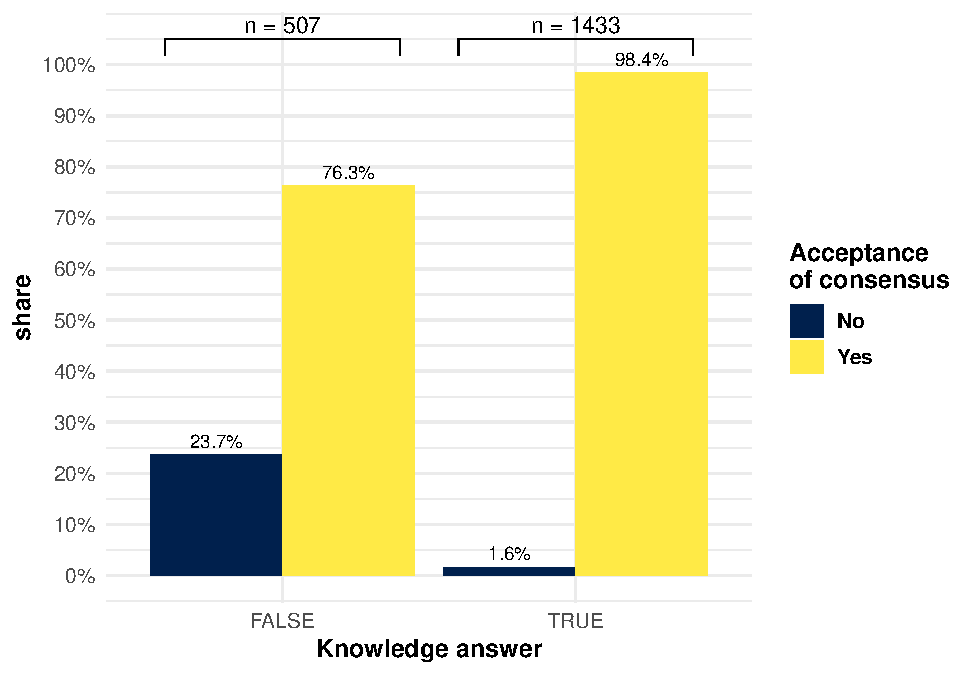
\includegraphics{output/figures/exp1-conditional-acceptance.pdf}
\caption{\label{fig:exp1-conditional-acceptance}Acceptance rates of scientific consensus, based on whether the initial response to the knowledge question was false or true.}
\end{figure}



\begin{figure}
\centering
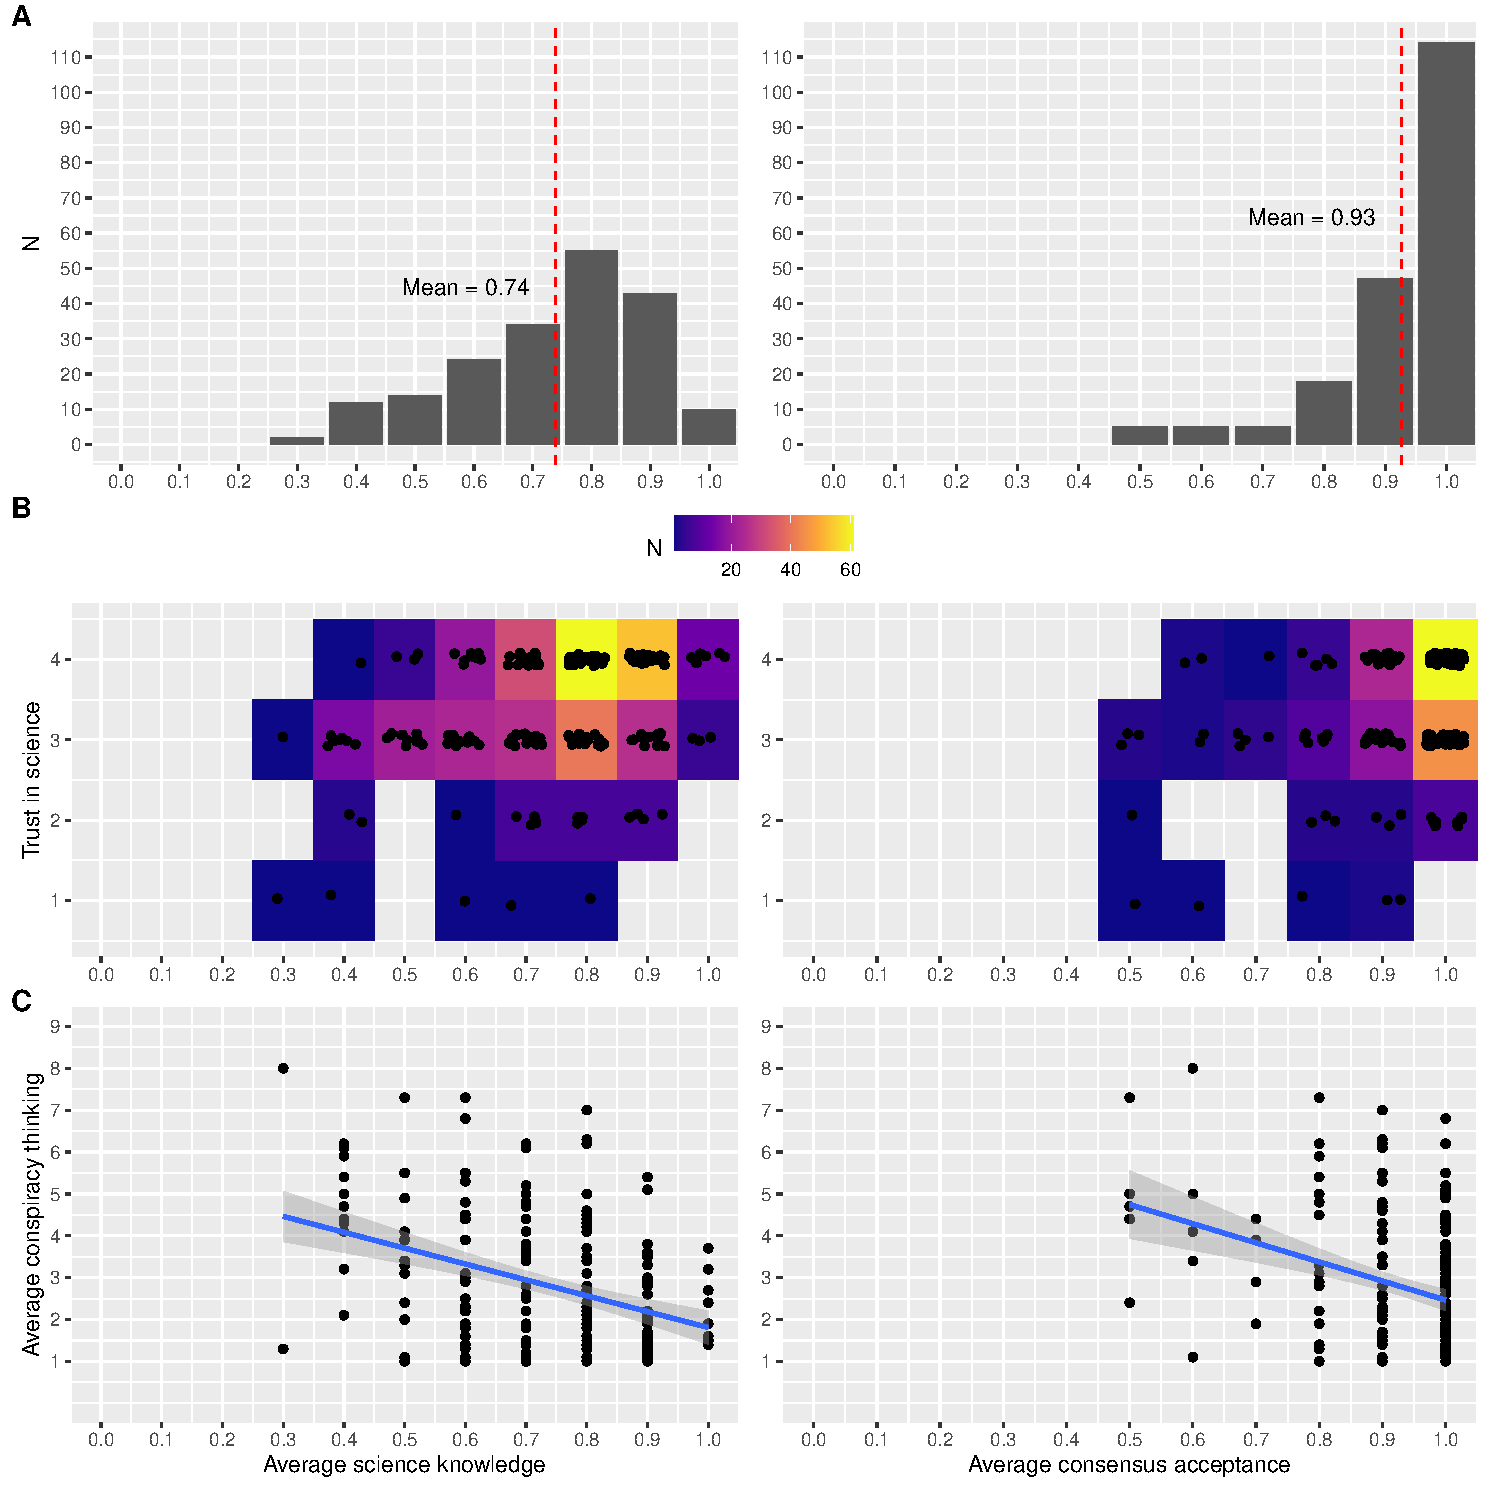
\includegraphics{output/figures/exp1-plot-overview.pdf}
\caption{\label{fig:exp1-plot-overview}\textbf{A} Shows the distribution of science knowledge (left) and acceptance of scientific consensus \textbf{B} Shows the relationship between trust in science and science knowledge/acceptance of scientific consensus \textbf{C} Shows the relationship between conspiracy thinking and science knowledge/acceptance of scientific consensus}
\end{figure}

\clearpage

\section{Experiment 2}\label{exp2}

In experiment 1, we tested whether participants would accept the scientific consensus on basic science facts. In most instances they did, but not always. In experiment 2, we wanted to test whether this reluctance was because of participants not trusting us as a source of consensual science knowledge. To do so, we added an explanation and sources to each consensus statement, instead of only stating the consensus. To better understand reasons for consensus rejection, after having answered all questions, we asked participants an open-ended question to explain why they rejected the consensus, for each question on which they did so. We also excluded the where do trees their materials from, as this question clearly seemed to be an outlier where most participants would get the answer wrong (see Appendix \ref{exp1}).

Based on experiment 1, we formulated the following hypotheses:

\textbf{H1a: Higher trust in science is associated with more science knowledge?}

\textbf{H1b: Higher trust in science is associated with more acceptance of the scientific consensus, for participants who did not already know it?}

\textbf{H2a: Higher conspiracy thinking is associated with less science knowledge?}

\textbf{H2b: Higher conspiracy thinking is associated with less acceptance of the scientific consensus, for participants who did not already know it?}

We had the following research questions:

\textbf{RQ1: What is the average science knowledge score?}

\textbf{RQ2: When a participant's answer does not match the consensus, how often do they change their mind and accept the consensus?}

\textbf{RQ3: What reasons do participants provide to justify their rejection of the scientific consensus?}

\subsection{Participants}\label{participants-2}

We recruited 201 participants from the US via prolific. 11 participants failed our attention check, resulting in a final sample of 190 participants (96 female, 94 male; \(age_\text{mean}\): 43.48, \(age_\text{sd}\): 12.25, \(age_\text{median}\): 42). Since we did not have any prior assumptions on effect sizes and our analyses were descriptive, we did not do a power analysis.

\subsection{Procedure}\label{procedure-1}

The procedure was the same as in experiment 1, with the difference that, instead of just stating the scientific consensus, participants were presented with a short explanation which we wrote, partly based on explanations generated by ChatGPT, and three links to authoritative sources supporting the answer (Fig. \ref{fig:exp2-stimulus-example}.

\subsection{Materials}\label{materials-3}

We relied on the same items as in experiment 1. The only difference was that we removed the question on trees.

\FloatBarrier



\begin{figure}

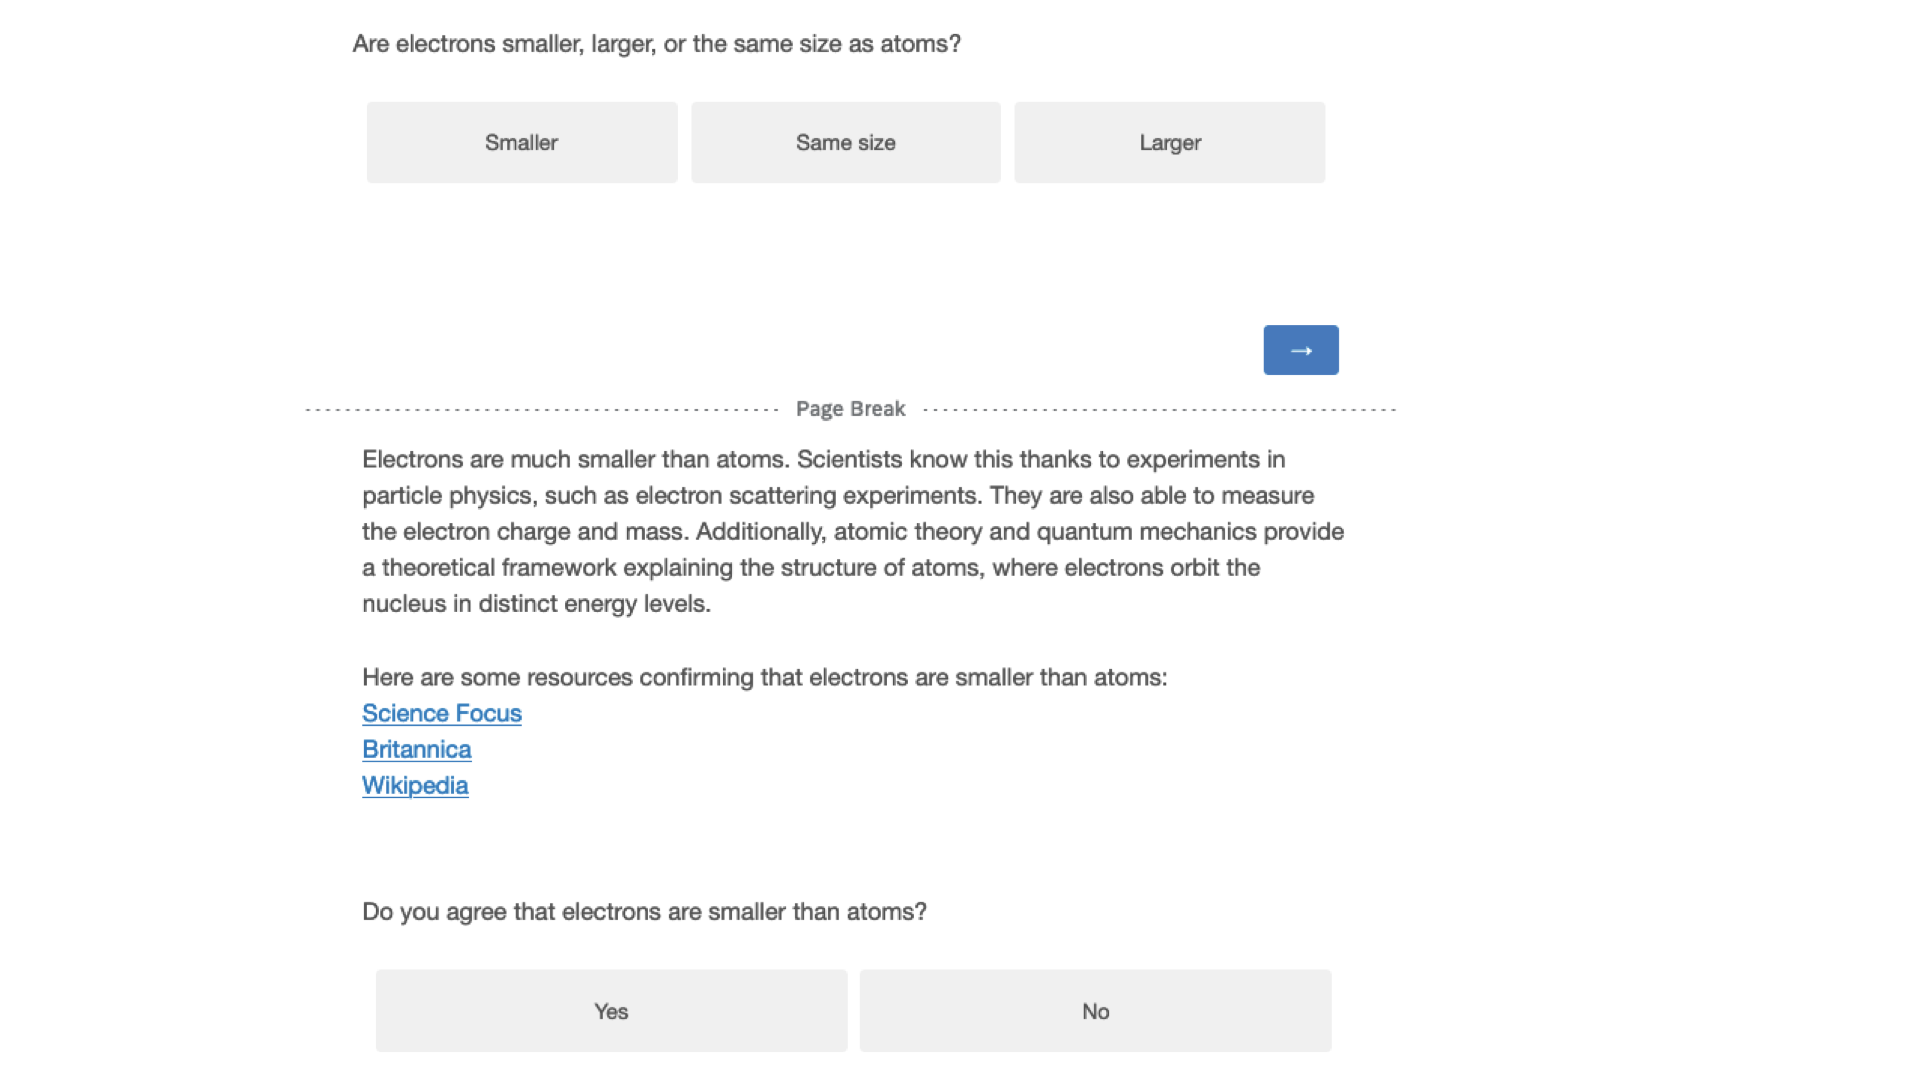
\includegraphics[width=1\linewidth]{./figures/study2_question_example} \hfill{}

\caption{Example of a science question, the scientific consensus and corresponding explanation and sources.}\label{fig:exp2-stimulus-example}
\end{figure}

\subsection{Results}\label{results-2}

As in experiment 1, we find a positive but small correlation between science knowledge and trust in science (H1a: r = 0.28, p \textless{} .001) and a small negative correlation between science knowledge and conspiracy thinking (H2a: r = -0.40, p \textless{} .001). By contrast to experiment 1, we conditioned on initially false answers when looking at the relationship of consensus acceptance with trust in science and conspiracy thinking, respectively. For trust in science, we find no statistically significant correlation (r = 0.16, p = 0.051). For conspiracy thinking we find a small negative one (r = -0.22, p = 0.006).

Confirming results from experiment 1, we find that the more people are knowledgeable about science and the more they tend to accept the scientific consensus even when they are not that knowledgeable in science, the more they tend to trust science. These correlations are relatively weak, which might be partly due to ceiling effects: As illustrated in Fig. \ref{fig:exp2-plot}, (i) most people do trust science, and (ii) that is true even among people with low knowledge or acceptance rates. In Appendix \ref{exp2} we show that these results hold for our alternative measures of trust and conspiracy thinking. We also include more descriptive statistics, such as knowledge and acceptance by science questions.

Regarding RQ1, participants answered on average 79 \% (sd = 0.19) of the questions correctly, and accepted the scientific consensus on average for 98 \% (sd = 0.05) of the questions. Fig. \ref{fig:exp2-conditional-acceptance} illustrates the relationship between knowledge and acceptance. In response to RQ2, in most cases (92.9 \%), participants readily accepted the scientific consensus after having initially given the wrong answer to a question. In very few cases (0.5 \%), participants who gave the correct response afterwards rejected the scientific consensus, thereby contradicting their own initial response.

\begin{table}[tbp]

\begin{center}
\begin{threeparttable}

\caption{\label{tab:exp2-justifications}Justifications by category}

\begin{tabular}{llll}
\toprule
Category & \multicolumn{1}{c}{N (instances)} & \multicolumn{1}{c}{Share (instances)} & \multicolumn{1}{c}{N (unique participants)}\\
\midrule
Personal convictions & 12.00 & 34.3\% & 8.00\\
Mistake & 9.00 & 25.7\% & 8.00\\
No justification & 7.00 & 20\% & 5.00\\
Not convinced & 5.00 & 14.3\% & 5.00\\
Religious Beliefs & 2.00 & 5.7\% & 2.00\\
\bottomrule
\end{tabular}

\end{threeparttable}
\end{center}

\end{table}

For RQ3, we got 35 answers from 25 different participants to the open-ended questions on why they had rejected the scientific consensus on a particular question. Table \ref{tab:exp2-justifications} summarizes these answers by five categories. All answers can be read in Appendix \ref{exp2}.

\subsection{Discussion}\label{discussion-2}

Similar to experiment 1, most people (i) do know and agree with the scientific consensus, and (ii) tend to accept the scientific consent even if they were not previously aware of it (i.e.~answered the knowledge question wrongly). The share of these latter is considerably larger in experiment 2 (92.9 \%) than in experiment 1 (76.3 \%). While this could be just sampling variation, it might be that adding explanations and sources convinced people more than merely stating the consensus. We also show, again, that people with lower trust in science and who believe more in conspiracy theories tend to both know less about science and accept the scientific consensus less.

\subsection{Comparing items}\label{comparing-items-1}

\subsubsection{Conspiracy theories}\label{conspiracy-theories-1}

Table \ref{tab:exp2-correlation-conspiracy} shows the correlations of the three different scales assessing conspiracy thinking.

\begin{table}[h]

\begin{center}
\begin{threeparttable}

\caption{\label{tab:exp2-correlation-conspiracy}Correlations of the three different scales assessing conspiracy thinking}

\begin{tabular}{llll}
\toprule
 & \multicolumn{1}{c}{BCTI} & \multicolumn{1}{c}{CMQ} & \multicolumn{1}{c}{SICBS}\\
\midrule
BCTI & 1.00 & 0.66 & 0.63\\
CMQ & 0.66 & 1.00 & 0.86\\
SICBS & 0.63 & 0.86 & 1.00\\
\bottomrule
\end{tabular}

\end{threeparttable}
\end{center}

\end{table}

\subsubsection{Trust in science}\label{trust-in-science-4}

Table \ref{tab:exp2-correlation-trust} shows the correlations of the three different items measuring trust in science.

\begin{table}[h]

\begin{center}
\begin{threeparttable}

\caption{\label{tab:exp2-correlation-trust}Correlations of the three different items measuring trust in science}

\begin{tabular}{llll}
\toprule
 & \multicolumn{1}{c}{wgm\_sciencegeneral} & \multicolumn{1}{c}{wgm\_scientists} & \multicolumn{1}{c}{pew}\\
\midrule
wgm\_sciencegeneral & 1.00 & 0.89 & 0.79\\
wgm\_scientists & 0.89 & 1.00 & 0.85\\
pew & 0.79 & 0.85 & 1.00\\
\bottomrule
\end{tabular}

\end{threeparttable}
\end{center}

\end{table}

\subsection{Correlations with alternative measures}\label{correlations-with-alternative-measures-1}

Table \ref{tab:exp2-correlations-outcomes} shows the correlations between knowledge and acceptance, respectively, and outcome variables.

\begin{table}[tbp]

\begin{center}
\begin{threeparttable}

\caption{\label{tab:exp2-correlations-outcomes}Correlations between knowledge and acceptance, respectively, and outcome variables}

\begin{tabular}{lll}
\toprule
outcome & \multicolumn{1}{c}{Correlation with knowledge} & \multicolumn{1}{c}{Correlation with acceptance}\\
\midrule
BCTI 
(main conspiracy measure) & -0.4 (p< .001) & -0.37 (p< .001)\\
CMQ & -0.17 (p= 0.019) & -0.22 (p= 0.003)\\
SICBS & -0.14 (p= 0.058) & -0.2 (p= 0.006)\\
WGM trust scientists & 0.23 (p= 0.002) & 0.25 (p< .001)\\
WGM trust general 
(main trust measure) & 0.28 (p< .001) & 0.3 (p< .001)\\
PEW trust scientists & 0.16 (p= 0.027) & 0.22 (p= 0.003)\\
\bottomrule
\end{tabular}

\end{threeparttable}
\end{center}

\end{table}

\subsection{Results conditional on false responses}\label{results-conditional-on-false-responses-1}

Table \ref{tab:exp2-false-response-regression} shows the correlations between acceptance and outcome variables based on linear regression models on standardized values.

\begin{table}

\caption{\label{tab:exp2-false-response-regression}Based on false response data only, correlations between acceptance and outcome variables based on linear regression models on standardized values}
\centering
\begin{tabular}[t]{lcccccc}
\toprule
  & BCTI\_avg & CMQ\_avg & SICBS & wgm\_scientists & wgm\_sciencegeneral & pew\\
\midrule
(Intercept) & 0.000 & 0.000 & 0.000 & 0.000 & 0.000 & 0.000\\
 & (0.081) & (0.080) & (0.081) & (0.082) & (0.082) & \vphantom{1} (0.082)\\
avg\_acceptance & -0.225** & -0.247** & -0.201* & 0.131 & 0.161+ & 0.130\\
 & (0.081) & (0.080) & (0.081) & (0.082) & (0.082) & (0.082)\\
\midrule
Num.Obs. & 147 & 147 & 147 & 147 & 147 & 147\\
R2 & 0.051 & 0.061 & 0.041 & 0.017 & 0.026 & 0.017\\
R2 Adj. & 0.044 & 0.054 & 0.034 & 0.010 & 0.019 & 0.010\\
AIC & 414.5 & 412.9 & 416.1 & 419.6 & 418.3 & 419.7\\
BIC & 423.5 & 421.9 & 425.0 & 428.6 & 427.3 & 428.6\\
Log.Lik. & -204.248 & -203.465 & -205.036 & -206.802 & -206.141 & -206.826\\
RMSE & 0.97 & 0.97 & 0.98 & 0.99 & 0.98 & 0.99\\
\bottomrule
\multicolumn{7}{l}{\rule{0pt}{1em}+ p $<$ 0.1, * p $<$ 0.05, ** p $<$ 0.01, *** p $<$ 0.001}\\
\end{tabular}
\end{table}

\subsection{By-question variation}\label{by-question-variation-1}

\subsubsection{Knowledge}\label{knowledge-1}



\begin{figure}
\centering
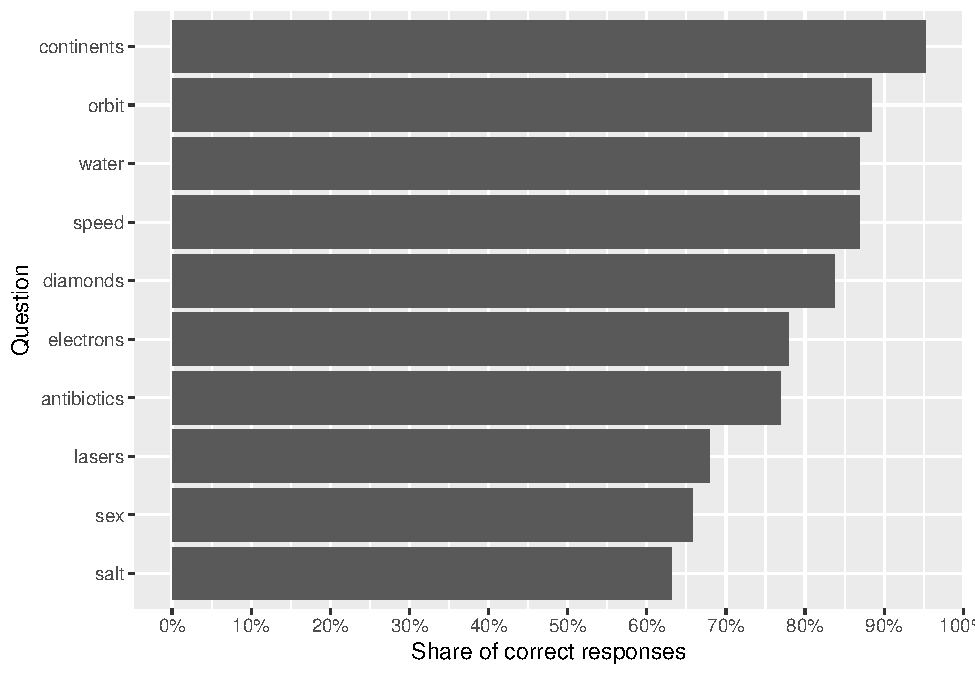
\includegraphics{output/figures/exp2-questions-knowledge.pdf}
\caption{\label{fig:exp2-questions-knowledge}Distribution of correct answers by question.}
\end{figure}

\subsubsection{Acceptance}\label{acceptance-1}



\begin{figure}
\centering
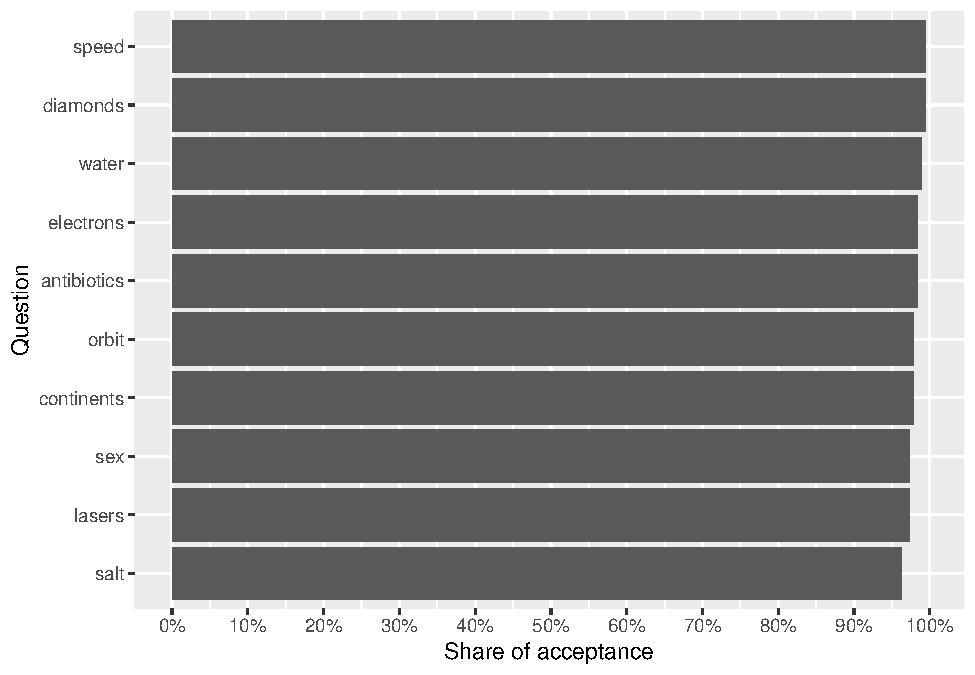
\includegraphics{output/figures/exp2-questions-acceptance.pdf}
\caption{\label{fig:exp2-questions-acceptance}Distribution of consensus acceptance by question.}
\end{figure}

\subsection{Trust in science}\label{trust-in-science-5}



\begin{figure}
\centering
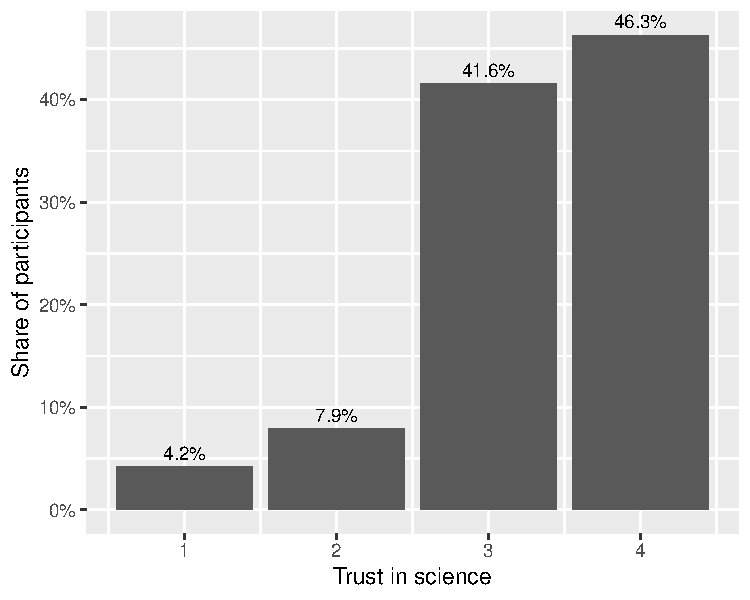
\includegraphics{output/figures/exp2-trust-scientists.pdf}
\caption{\label{fig:exp2-trust-scientists}Distribution of trust in scientists.}
\end{figure}

\subsection{Conspiracy thinking}\label{conspiracy-thinking-2}

\subsubsection{Distribution}\label{distribution-1}



\begin{figure}
\centering
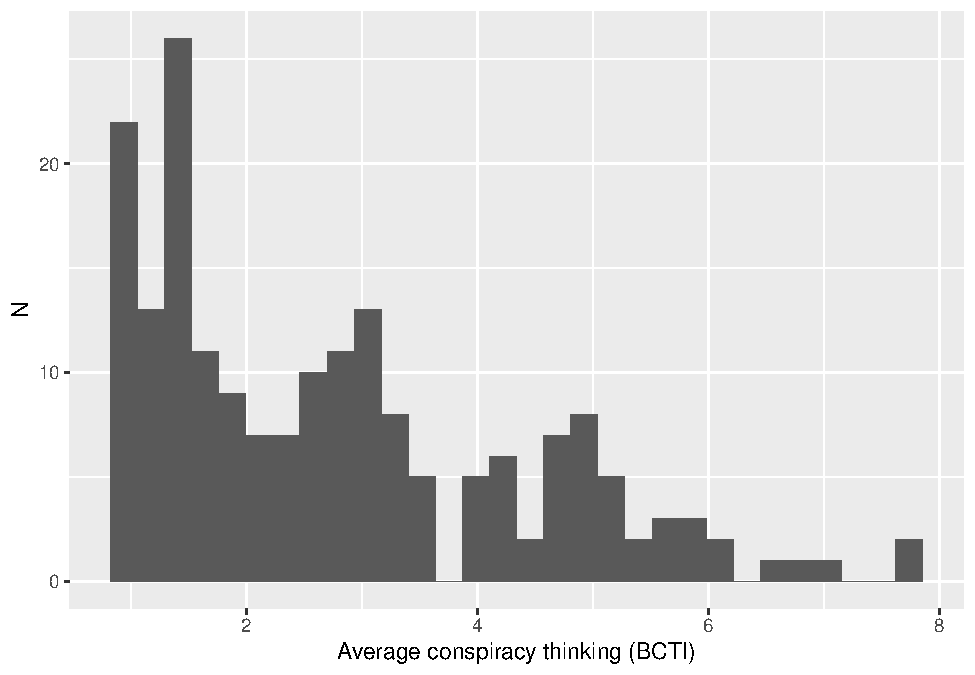
\includegraphics{output/figures/exp2-conspiracy-distribution.pdf}
\caption{\label{fig:exp2-conspiracy-distribution}Distribution of conspiracy thinking.}
\end{figure}

\subsubsection{By-item variation}\label{by-item-variation-1}



\begin{figure}
\centering
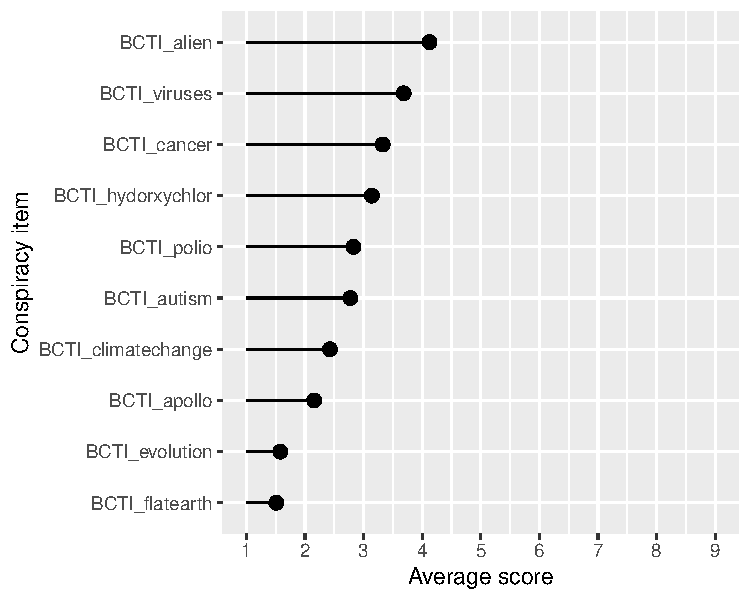
\includegraphics{output/figures/exp2-conspiracy-items.pdf}
\caption{\label{fig:exp2-conspiracy-items}Distribution of conspiracy thinking by item.}
\end{figure}

\subsection{Reasons for consensus rejection}\label{reasons-for-consensus-rejection}

\subsubsection{By category}\label{by-category}

{[}To do{]}

\subsubsection{All raw answers}\label{all-raw-answers}

\begin{longtable}[t]{>{}r>{}l>{\raggedright\arraybackslash}p{30em}}
\caption{\label{tab:exp2-reasons-rejection}Reasons for consensus rejection}\\
\toprule
id & question & answer\\
\midrule
33 & sex & Because I didn't think the information provided here was accurate, more or less.\\
45 & lasers & I read the article.\\
45 & salt & Read the article provided.\\
47 & lasers & The statement "lasers do not work by focusing sound waves" is correct according to scientific consensus. Lasers operate on the principles of stimulated emission of radiation, wherein photons are emitted in a coherent, focused beam through the process of stimulated emission.\\
47 & diamonds & Are diamonds made of carbon? Scientific consensus: Diamonds are made of carbon.  Do you think you could explain why you answered differently?\\
\addlinespace
47 & water & it likely arose from a mistake or miscommunication.\\
50 & orbit & I honestly couldn't remember.\\
50 & speed & When I looked it up I got two different answers.\\
71 & water & After I put "No", I realized that I was thinking about "H2o" incorrectly. So yes, I actually do agree.\\
73 & electrons & Atoms are known to be the smallest unit of matter.\\
\addlinespace
77 & continents & I believe God make it they way it is and if He wanted it changed, He would have done it\\
78 & sex & no\\
78 & salt & no\\
79 & orbit & It’s early and I’m tired. I misread it.\\
105 & salt & I think I simply misunderstood the paragraph. I'm actually trying to read it thoroughly and answering truthfully, but I have misread it.\\
\addlinespace
109 & electrons & Maybe\\
127 & continents & I'm a young earth Christian. I believe the Christian Bible (and outside sources) offers ample evidence that the earth is thousands of years old, not millions.\\
127 & orbit & I do not believe in the heliocentric model of an earth spinning around a centralized sun.\\
130 & continents & I don't think the continent move rather it is the atmosphere\\
130 & sex & I think that the gene both parent release should determine the sex of the baby\\
\addlinespace
131 & antibiotics & There are some antibiotics that also kill viruses\\
132 & salt & Because it says that table salt is not made of calcium carbonate, so I clicked no.\\
133 & lasers & I feel like the excerpt that was provided did not definitively state the answer.\\
140 & lasers & It was confusing to understand the explanation of why lasers don’t focus on sound\\
152 & continents & I think that they were that way after the ice age.  It split apart the whole surface and then water filled in and they have remained the same for ever.  They are not moving around or have they for millions of years.\\
\addlinespace
152 & orbit & The  Earth circles the sun every day.  The dark side is when the moon comes out.  So everyday, you have daylight and dark (moon).  Dark comes from the dark side of the sun.\\
170 & lasers & I may have misread, but I did not see confirmation of this.\\
172 & salt & no\\
178 & electrons & This answer is different because atoms is everywhere and you can't see it but electrons aren't out that as much at all but you could possibly know it's there\\
178 & antibiotics & Because antibiotics can kill bacteria in which kills the virus as well in the process so you get healed with this product\\
\addlinespace
178 & sex & There is no 100\% evidence that this is the case and I still fully believe that it is from both genes to make this decision.\\
179 & antibiotics & Antibiotics seem that if they are capable of killing tiny things such as bacteria then they are most likely to attach to other things in out bodies and cause it harm although unintentional.\\
183 & salt & I thought the scientific consensus was right\\
186 & sex & The scientific consensus is clear: both parents' genes determine the sex of a baby, specifically the sex chromosomes they contribute.\\
189 & salt & I made an error in my selection.\\
\bottomrule
\end{longtable}

\subsection{Additional plots}\label{additional-plots-1}



\begin{figure}
\centering
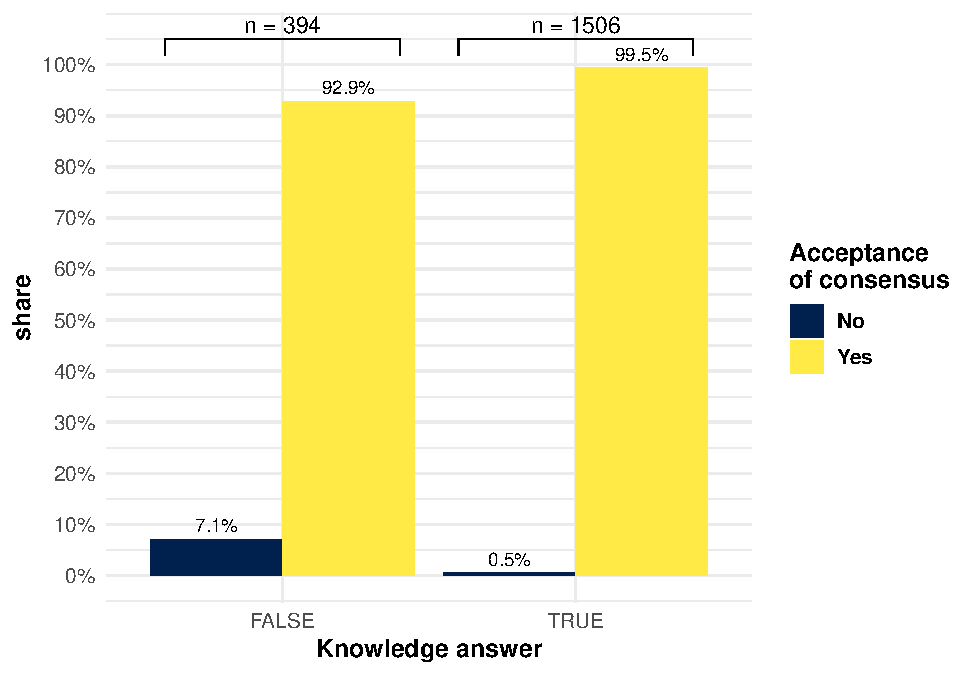
\includegraphics{output/figures/exp2-conditional-acceptance.pdf}
\caption{\label{fig:exp2-conditional-acceptance}Acceptance rates of scientific consensus, based on whether the initial response to the knowledge question was false or true.}
\end{figure}




\clearpage

\section{Experiment 3}\label{exp3}

Study 3 is essentially a replication-\/--with some minor modifications-\/--of study 2, but on a different type of sample. Both study 1 and 2 were run on convenience samples. For study 3, we recruited a sample of people holding anti-vaccination beliefs (see below). By contrast to study 2, after asking participants an open question about why they did not accept the consensus (in cases where they didn't), we provide them with an explicit opportunity to change their answer (Fig. \ref{fig:exp3-explanation-example}). Based on the answers to the open-ended questions, we also pre-registered a categorization scheme of reasons why people rejected the consensus. Finally, we also ask participants about why they agree with the scientific consensus on certain questions, in case they do. We want to know if participants perceive that this is because of trust, or other factors.

As for study 2 (but without conditioning on wrong answers, as we did in study 1), we had the following hypotheses:

\textbf{H1a: Higher trust in science is associated with more science knowledge?}

\textbf{H1b: Higher trust in science is associated with more acceptance of the scientific consensus.}

\textbf{H2a: Higher conspiracy thinking is associated with less science knowledge?}

\textbf{H2b: Higher conspiracy thinking is associated with less acceptance of the scientific consensus.}

We had the following research questions:

\textbf{RQ1: What is the average science knowledge score?}

\textbf{RQ2: What is the average acceptance of the scientific consensus}

\textbf{RQ3: What reasons do participants provide to justify their rejection of the scientific consensus?}

\textbf{RQ4: In case they agree with the scientific consensus, do people feel that this is because of trust?}

\subsection{Participants}\label{participants-3}

We recruited a sample of participants holing vaccine-skeptic beliefs. Prolific Academic allows to filter out participants who have given specific answers to certain questions. We selected three available questions: 1. ``Participants were asked the following question: Please describe your attitudes towards the COVID-19 (Coronavirus) vaccines: {[}For (I feel positively about the vaccines); Against (I feel negatively about the vaccines); Neutral (I don't have strong opinions either way); Prefer not to say''{]}. We selected particpants who answered''Against''. 2. ``Participants were asked the following question: Have you received a coronavirus (COVID-19) vaccination? {[}Yes (at least one dose); No; Prefer not to answer{]}''. We select only people who answered ``No''. 3. ``Participants were asked the following question: On a scale from 1-7, please rate to what extent you agree with the following statement: I believe that scheduled immunizations are safe for children. {[}1 (TOTALLY DISAGREEE); 2 (DISAGREE); 3 (SOMEWHAT DISAGREE); 4 (NEITHER AGREE NOR DISAGREE); 5 (SOMEWHAT AGREE); 6 (AGREE); 7 (TOTALLY AGREE); Rather not say''{]}. We select only people who answered''1'', ``2'', or ``3''.

Based on these criteria, we recruited 200 participants from the US via prolific, of which none failed our attention check, resulting in a final sample of 200 participants (125 female, 73 male; \(age_\text{mean}\): 42.90, \(age_\text{sd}\): 12.00, \(age_\text{median}\): 41). Since we did not have any prior assumptions on effect sizes and our analyses were descriptive, we did not do a power analysis.

However, due to a randomization mistake for our outcomes, participant answered only two of the three outcome measure blocs (trust in science, conspiracy thinking, and reason for accepting consensus). This leaves us with reduced sample sizes for all analyses concerning these outcomes (N = 140 for trust in science, N = 138 for conspiracy measures, N = 122 for reason for accepting consensus).

\subsection{Procedure}\label{procedure-2}

The procedure was mostly the same as in experiment 2. In addition, after each open-ended question on cases where participants rejected the scientific consensus, participants were also asked if they want to change their answer and accept the scientific consensus. Finally, at the end of the survey, we asked participants: ``For the questions in which you agreed with the scientific consensus, would you say that\ldots?'' The answer options were: (i) ``You mostly agree with the consensus because, on that question, you trust scientists'', (ii) ``You mostly agree with the consensus because you have been able to independently verify it'', and (iii) ``Other'', with a text box for participants to explain. Participants who selected ``You mostly agree with the consensus because you have been able to independently verify it'', were asked the open-ended follow-up question: ``Could you please tell us how you independently verified the information?''.

\subsection{Materials}\label{materials-4}

\FloatBarrier



\begin{figure}

{\centering 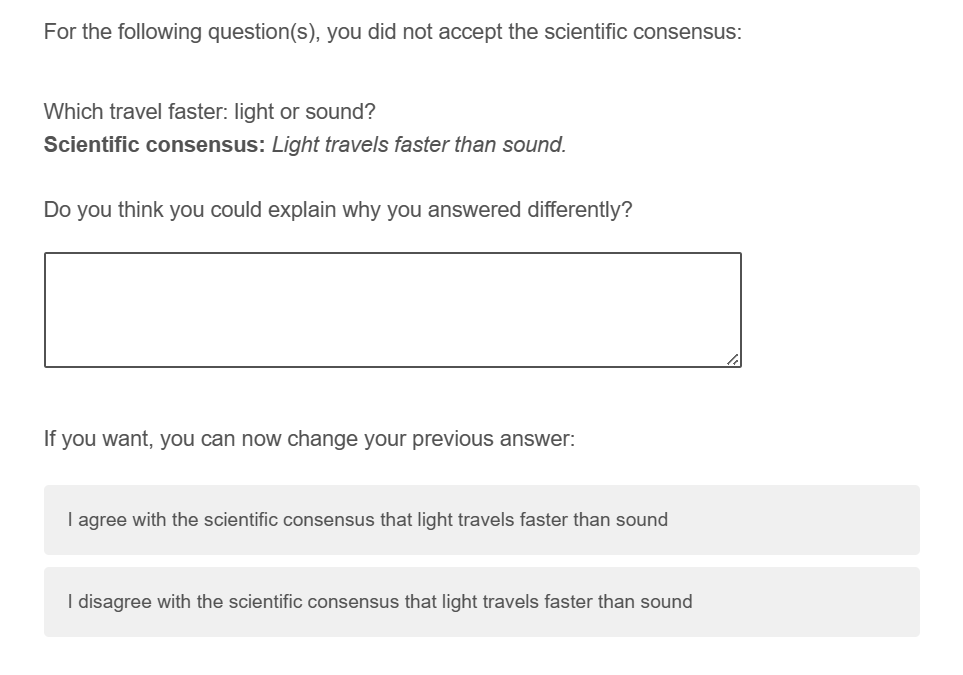
\includegraphics[width=0.5\linewidth]{figures/study3_example_explanation} 

}

\caption{Example of an explanation question and the opportunity to change the previous answer.}\label{fig:exp3-explanation-example}
\end{figure}

Table \ref{tab:knowledge-overview} shows all questions, their scientifically consensual answer, and their source. All but two questions were selected from existing science knowledge questionnaires. We tried to select non-political questions.

\begingroup\fontsize{8}{10}\selectfont

\begin{longtable}[t]{>{\raggedleft\arraybackslash}p{1em}>{\raggedright\arraybackslash}p{10em}>{\raggedright\arraybackslash}p{10em}>{\raggedright\arraybackslash}p{23em}}
\caption{\label{tab:knowledge-overview}Science knowledge items}\\
\toprule
id & Question & Scientific consensus (Study 1) & Explanation (Study 2 \& 3)\\
\midrule
1 & Do antibiotics kill viruses as well as bacteria? & There is a consensus among scientists that antibiotics kill bacteria, but not viruses. & Antibiotics specifically target and kill bacteria, not viruses. Scientists know this thanks to extensive laboratory experiments and clinical trials where antibiotics have been observed to be effective against bacterial infections but not viral ones. Scientists have also studied how antibiotics work, which typically involve disrupting bacterial cell processes like cell wall synthesis or protein production, which are absent in viruses.

Here are some resources confirming that antibiotics only kill bacteria: 
American Chemical Society
Queensland Government 
Wikipedia\\
2 & Are electrons smaller, larger, or the same size as atoms ? & There is a consensus among scientists that electrons are smaller than atoms. & Electrons are much smaller than atoms. Scientists know this thanks to experiments in particle physics, such as electron scattering experiments. They are also able to measure the electron charge and mass. Additionally, atomic theory and quantum mechanics provide a theoretical framework explaining the structure of atoms, where electrons orbit the nucleus in distinct energy levels.

Here are some resources confirming that electrons are smaller than atoms:
Science Focus 
Britannica 
Wikipedia\\
3 & Have the continents on Earth been moving for millions of years or have they always been where they are now? & There is a consensus among scientists that the continents on Earth have been moving for millions of years due to plate tectonics. & The continents on Earth have been moving for millions of years due to plate tectonics. Scientists have gathered evidence from various sources, including fossil records, geological formations, and the magnetic properties of rocks. The theory of plate tectonics explains how the Earth's lithosphere is divided into large, rigid plates that move over the semi-fluid asthenosphere, leading to phenomena like continental drift, earthquakes, and volcanic activity.

Here are some resources confirming that continents on Earth have been moving for millions years:
Britannica 
Live Science 
National Geographic\\
4 & What decides whether a baby is a boy or a girl ? Is it the father’s genes, the mother’s genes, or both? & There is a consensus among scientists that it is the genes in the father's sperm which are decisive on whether a baby is a boy or a girl. & Chromosomes are structures found in the nucleus of cells that carry long pieces of DNA. Two of the chromosomes (the X and the Y chromosome) are called sex chromosomes. In most cases, females have two X chromosomes, while males have one X and one Y chromosome. At conception, the mother transmits an X chromosome, and the father may contribute an X or a Y. The chromosome from the father therefore determines if the baby is female (if the father transmits an X) or male (if the father transmits a Y). In most cases, children are born a male or female according to their chromosomes. However, some children may be born with genitalia that do not match their chromosomes.

Here are some resources confirming that it is the father's genes that decide the sex of a baby: 
National Library of Medicine 
Nature 
Wikipedia\\
5 & Do lasers work by focusing sound waves? & There is a consensus among scientists that lasers do not work by focusing sound waves. & Lasers produce a narrow beam of light in which all of the particles of light have very similar wavelengths. The laser’s lightwaves travel together with their peaks all lined up, in phase. This is why laser beams are very narrow, very bright, and can be focused into a very tiny spot. Because laser light stays focused and does not spread out much (like a flashlight would), laser beams can travel very long distances.

Here are some resources confirming that lasers do not work by focusing sound waves: 
NASA 
Lawrence Livermore National Library
Wikipedia\\
\addlinespace
6 & How long does it take for Earth to go around the sun: one day, one month, or one year ? & There is a consensus among scientists that it takes one year for Earth to go around the sun. & Earth takes approximately one year to orbit the sun. This knowledge is based on astronomical observations and measurements of celestial motion. Early astronomers tracked the movement of the Earth relative to the stars and planets, leading to the development of models that accurately predict the Earth's orbital period around the sun.

Here are some resources confirming that Earth goes around the sun in one year: 
NASA
National Geographic 
Wikipedia\\
7 & Are diamonds made of carbon ? & There is a consensus among scientists that diamonds are made of carbon. & Diamonds are made of only one element, carbon. Carbon is the same element that makes coal or graphite used for pencils. Why are diamonds transparent and hard while coal and graphite are opaque and soft? It all comes down to the placement of their atoms. In diamonds, each carbon atom is bonded to 4 other carbon atoms, while in graphite, each atom is only bonded to 3 other carbon atoms. The bonds in diamonds are held in such a tight structure that all light passes around them, which is why diamonds look transparent. In coal and graphite, light gets trapped between the atoms, which is why they look dark and opaque. Why do carbon atoms bond differently in diamonds? At very high pressures and temperatures, the carbon atoms are squeezed so much that they start touching more atoms. When the pressure is about 50,000 times the pressure at the surface of the Earth and the temperature is about 1600°C, the carbon atoms bond with 4 other atoms and result in diamonds.

Here are some resources confirming that diamonds are made of carbon: 
Arizona State University 
University of Bristol 
Wikipedia\\
8 & Which travels faster : light or sound? & There is a consensus among scientists that light travels faster than sound. & Light travels faster than sound. This conclusion arises from numerous experiments and observations in physics. You can also experience this for yourself during a thunderstorm. Unless the lighting is right above you, you will first see the lighting, then hear the thunder some time after (you can even tell how far the lighting struck by counting how many seconds it takes for the thunder to reach you). More precisely, the speed of light has been measured accurately using techniques such as the Michelson–Morley experiment. Similarly, the speed of sound has been measured through experiments involving the propagation of sound waves through various materials.

Here are some resources confirming that light travers faster than sound: 
NASA 
Wikipedia : Speed of light 
Wikipedia: Speed of sound\\
9 & Is common table salt made of calcium carbonate? & There is a consensus among scientists that common table salt is not made of calcium carbonate; it is made of sodium chloride. & Common table salt, or sodium chloride (NaCl), is not made of calcium carbonate. Scientists can use a variety of tests to understand what matter is made of. The most used test for sodium chloride is the chemical reaction with silver nitrate. The presence of sodium chloride yields a white precipitate upon drops of a silver nitrate solution. Calcium carbonate, by contrast, is the substance that makes up, for instance, chalk.

Here are some resources confirming that common table salt is not made of calcium carbonate: 
National Library of Medicine 
Chem Europe 
Wikipedia\\
10 & Is water made of molecules containing one oxygen and two hydrogen atoms? & There is a consensus among scientists that water is made of molecules containing one oxygen and two hydrogen atoms, and that its chemical formula is therefore H2O. & Water is made of molecules containing one oxygen atom and two hydrogen atoms, chemically represented as H2O. We know this for instance because if you set hydrogen on fire in a container with oxygen, water will form on the sides of the container. More recent techniques such as spectroscopy and X-ray crystallography have allowed scientists to more directly see the composition and structure of water molecules, confirming the presence of two hydrogen atoms bonded to one oxygen atom.

Here are some resources confirming that water is made of molecules containing one oxygen and two hydrogen atoms:
National Library of Medicine 
Wikipedia: Chemical structure 
Wikipedia: Water\\
\addlinespace
11 & Where do trees mainly draw the materials with which they create their mass? & There is a consensus among scientists that carbon drawn from the air during photosynthesis makes up most of the materials that trees use to build new leaves, stems, and roots. & \\
\bottomrule
\end{longtable}
\endgroup{}

\subsection{Results}\label{results-3}

As in study 1 and 2, we find that participants answered on average 75 \% (sd = 0.18) of the questions correctly (RQ1), and initially accepted the scientific consensus on average for 96 \% (sd = 0.08) of the questions (RQ2). The acceptance rate is even higher when accounting for opinion revisions towards acceptance of the consensus, after initial rejection (98 \%, sd = 0.06).

Fig. \ref{fig:exp3-conditional-acceptance} illustrates the relationship between knowledge and acceptance. In most cases (87 \%), participants readily accepted the scientific consensus right after having given the wrong answer to a question. After providing the chance to revise the initial consensus rejection, this share is even larger (95.5 \%). In very few cases (0.9 \%), participants who initially gave the correct response afterwards rejected the scientific consensus right after, thereby contradicting their own initial response. This share drops slightly after providing the chance to revise the initial consensus rejection (0.7 \%).

For all correlations, we include opinion revisions for measuring consensus acceptance. We find no statistically significant correlation between science knowledge and trust in science (r = 0.14, p = 0.100), but a samll positive correlation between acceptance of scientific consensus and trust in science (r = 0.20, p = 0.019). Again, these findings might be partly due to ceiling effects: As illustrated in Fig. \ref{fig:exp3-plot}, (i) most people do trust science, and (ii) that is true even among people with low knowledge or acceptance rates. We find no statistically significant correlation between conspiracy thinking and science knowledge (r = -0.16, p = 0.055), and between conspiracy thinking and acceptance of scientific consensus (r = -0.02, p = 0.788).

For RQ3, we got 74 answers from 47 different participants to the open-ended questions on why they had rejected the scientific consensus on a particular question. Table \ref{tab:exp3-justifications} summarizes these answers by five categories.

All answers can be read in the appendix.

\begin{table}[tbp]

\begin{center}
\begin{threeparttable}

\caption{\label{tab:exp3-justifications}Justifications by category}

\begin{tabular}{llll}
\toprule
Category & \multicolumn{1}{c}{N (instances)} & \multicolumn{1}{c}{Share (instances)} & \multicolumn{1}{c}{N (unique participants)}\\
\midrule
Personal convictions & 25.00 & 33.8\% & 19.00\\
Mistake & 21.00 & 28.4\% & 18.00\\
No justification & 18.00 & 24.3\% & 13.00\\
Not convinced & 7.00 & 9.5\% & 3.00\\
Religious Beliefs & 3.00 & 4.1\% & 3.00\\
\bottomrule
\end{tabular}

\end{threeparttable}
\end{center}

\end{table}

For RQ4, we had 122 participants answering the question. Of these 41.8\% said they accepted the scientific consensus because they trust scientists on this question, while 47.5\% said they independently verified the fact. 10.7\% answered with other ``other'' and gave an open-ended explanation (see below for all open-ended answers).

We also asked all 58 participants who answered that they had independently verified the answer to explain how they did so. The open-ended answers are listed below.

\subsection{Comparing items}\label{comparing-items-2}

\subsubsection{Conspiracy theories}\label{conspiracy-theories-2}

Table \ref{tab:exp3-correlation-conspiracy} shows the correlations of the three different scales assessing conspiracy thinking.

\begin{table}[h]

\begin{center}
\begin{threeparttable}

\caption{\label{tab:exp3-correlation-conspiracy}Correlations of the three different scales assessing conspiracy thinking}

\begin{tabular}{llll}
\toprule
 & \multicolumn{1}{c}{BCTI} & \multicolumn{1}{c}{CMQ} & \multicolumn{1}{c}{SICBS}\\
\midrule
BCTI & 1.00 & NA & NA\\
CMQ & NA & 1.00 & NA\\
SICBS & NA & NA & 1.00\\
\bottomrule
\end{tabular}

\end{threeparttable}
\end{center}

\end{table}

\subsubsection{Trust in science}\label{trust-in-science-6}

Table \ref{tab:exp3-correlation-trust} shows the correlations of the three different items measuring trust in science.

\begin{table}[h]

\begin{center}
\begin{threeparttable}

\caption{\label{tab:exp3-correlation-trust}Correlations of the three different items measuring trust in science}

\begin{tabular}{llll}
\toprule
 & \multicolumn{1}{c}{wgm\_sciencegeneral} & \multicolumn{1}{c}{wgm\_scientists} & \multicolumn{1}{c}{pew}\\
\midrule
wgm\_sciencegeneral & 1.00 & 0.77 & 0.68\\
wgm\_scientists & 0.77 & 1.00 & 0.68\\
pew & 0.68 & 0.68 & 1.00\\
\bottomrule
\end{tabular}

\end{threeparttable}
\end{center}

\end{table}

\subsection{Correlations with alternative measures}\label{correlations-with-alternative-measures-2}

Table \ref{tab:exp3-correlations-outcomes} shows the correlations between knowledge and acceptance, respectively, and outcome variables.

\begin{table}[tbp]

\begin{center}
\begin{threeparttable}

\caption{\label{tab:exp3-correlations-outcomes}Correlations between knowledge and acceptance, respectively, and outcome variables}

\begin{tabular}{lll}
\toprule
outcome & \multicolumn{1}{c}{Correlation with knowledge} & \multicolumn{1}{c}{Correlation with acceptance}\\
\midrule
BCTI 
(main conspiracy measure) & -0.16 (p= 0.055) & -0.03 (p= 0.788)\\
CMQ & 0.01 (p= 0.925) & -0.01 (p= 0.934)\\
SICBS & 0.02 (p= 0.767) & 0 (p= 0.987)\\
WGM trust scientists & 0.11 (p= 0.193) & 0.2 (p= 0.007)\\
WGM trust general 
(main trust measure) & 0.14 (p= 0.100) & 0.17 (p= 0.019)\\
PEW trust scientists & -0.08 (p= 0.367) & 0.12 (p= 0.104)\\
\bottomrule
\end{tabular}

\end{threeparttable}
\end{center}

\end{table}

\subsection{Results conditional on false responses}\label{results-conditional-on-false-responses-2}

Table \ref{tab:exp3-false-response-regression} shows the correlations between acceptance and outcome variables based on linear regression models on standardized values.

\begin{table}

\caption{\label{tab:exp3-false-response-regression}Based on false response data only, correlations between acceptance and outcome variables based on linear regression models on standardized values}
\centering
\begin{tabular}[t]{lcccccc}
\toprule
  & BCTI\_avg & CMQ\_avg & SICBS & wgm\_scientists & wgm\_sciencegeneral & pew\\
\midrule
(Intercept) & -0.001 & 0.000 & 0.000 & 0.005 & 0.002 & 0.008\\
 & (0.091) & (0.091) & (0.091) & (0.088) & (0.089) & (0.088)\\
avg\_acceptance & -0.043 & -0.025 & -0.009 & 0.083 & 0.039 & 0.125\\
 & (0.090) & (0.090) & (0.090) & (0.079) & (0.079) & (0.078)\\
\midrule
Num.Obs. & 122 & 122 & 122 & 128 & 128 & 128\\
R2 & 0.002 & 0.001 & 0.000 & 0.009 & 0.002 & 0.020\\
R2 Adj. & -0.006 & -0.008 & -0.008 & 0.001 & -0.006 & 0.012\\
AIC & 351.0 & 351.1 & 351.2 & 367.1 & 368.0 & 365.7\\
BIC & 359.4 & 359.6 & 359.6 & 375.7 & 376.5 & 374.2\\
Log.Lik. & -172.491 & -172.571 & -172.604 & -180.560 & -180.996 & -179.843\\
RMSE & 0.99 & 1.00 & 1.00 & 0.99 & 1.00 & 0.99\\
\bottomrule
\multicolumn{7}{l}{\rule{0pt}{1em}+ p $<$ 0.1, * p $<$ 0.05, ** p $<$ 0.01, *** p $<$ 0.001}\\
\end{tabular}
\end{table}

\subsection{By-question variation}\label{by-question-variation-2}

\subsubsection{Knowledge}\label{knowledge-2}



\begin{figure}
\centering
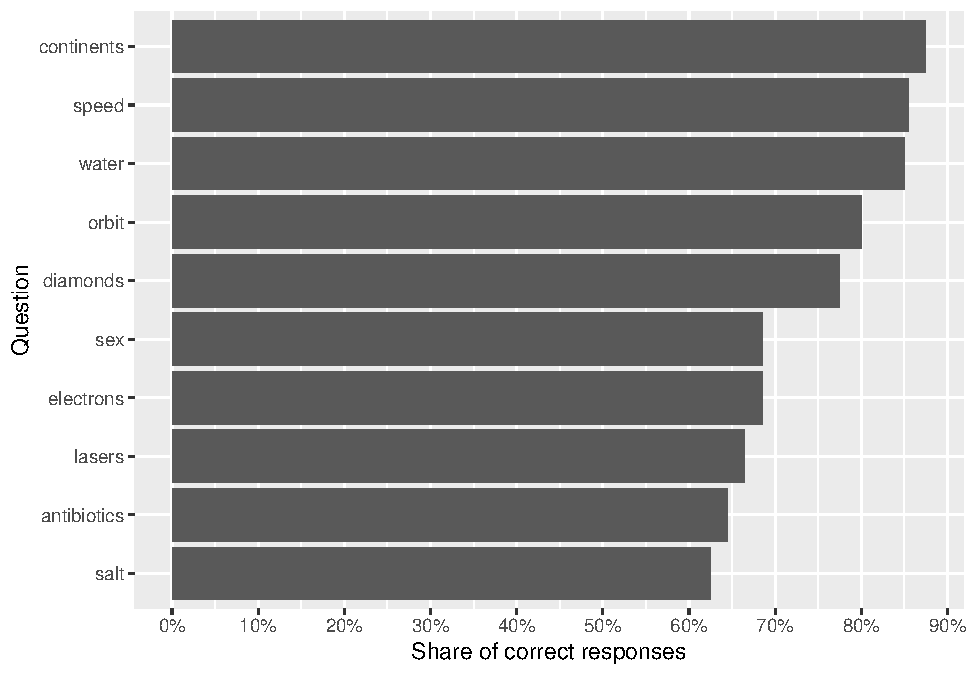
\includegraphics{output/figures/exp3-questions-knowledge.pdf}
\caption{\label{fig:exp3-questions-knowledge}Distribution of correct answers by question.}
\end{figure}



\begin{figure}
\centering
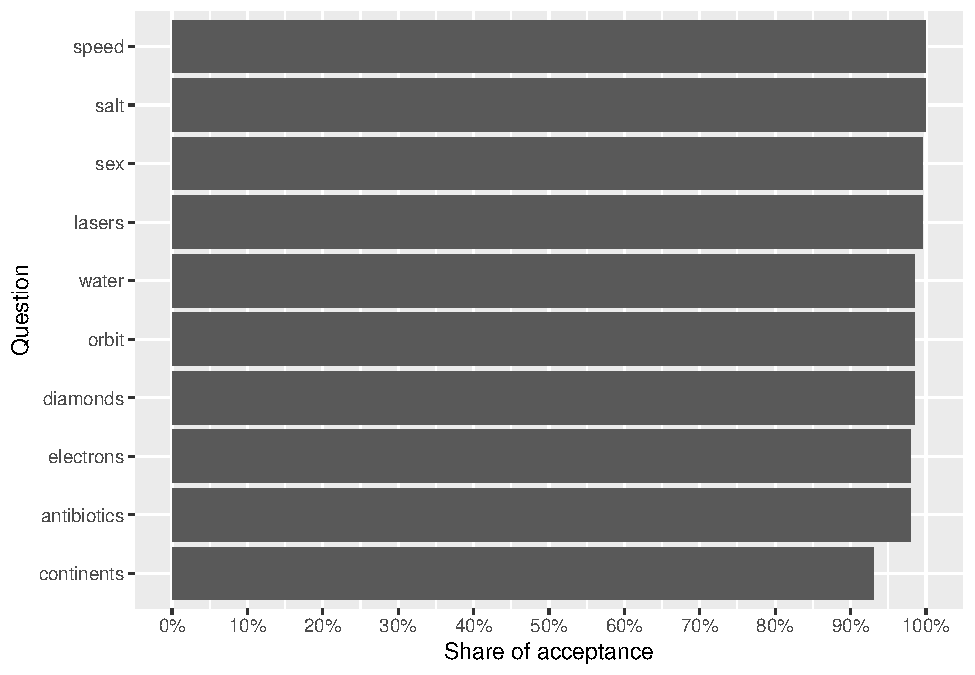
\includegraphics{output/figures/exp3-questions-acceptance.pdf}
\caption{\label{fig:exp3-questions-acceptance}Distribution of consensus acceptance by question.}
\end{figure}

\subsection{Trust in science}\label{trust-in-science-7}



\begin{figure}
\centering
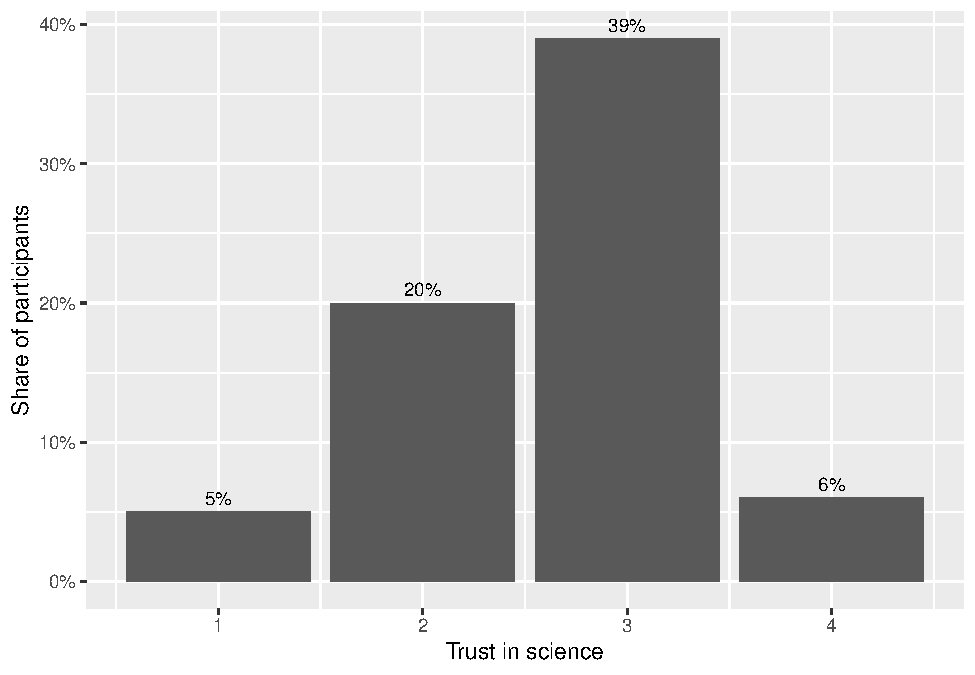
\includegraphics{output/figures/exp3-trust-scientists.pdf}
\caption{\label{fig:exp3-trust-scientists}Distribution of trust in scientists.}
\end{figure}

\subsection{Conspiracy thinking}\label{conspiracy-thinking-3}



\begin{figure}
\centering
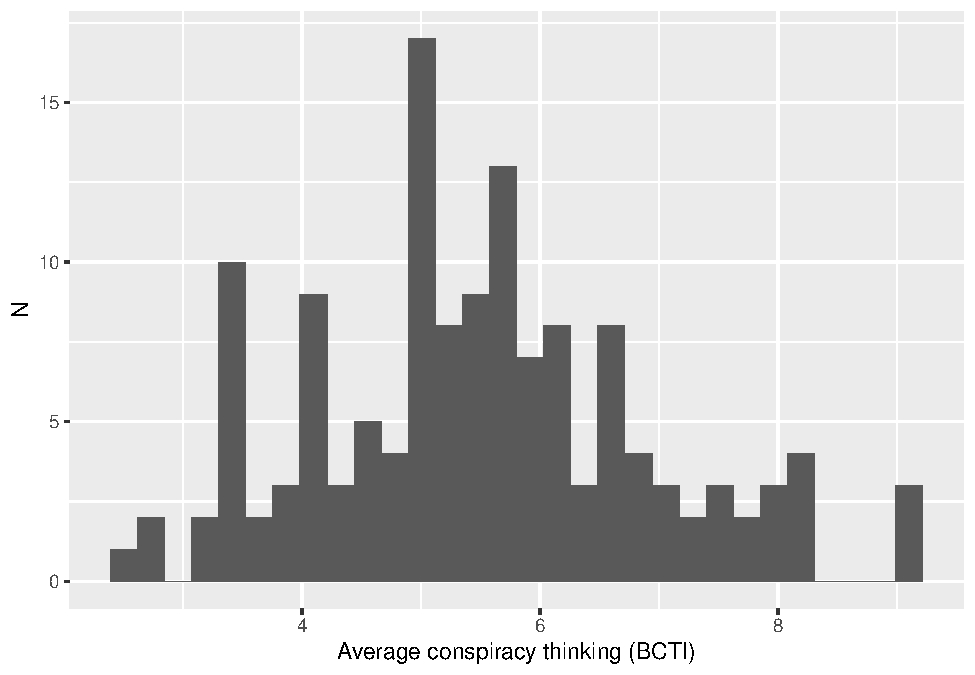
\includegraphics{output/figures/exp3-conspiracy-distribution.pdf}
\caption{\label{fig:exp3-conspiracy-distribution}Distribution of conspiracy thinking.}
\end{figure}

\subsubsection{By-item variation}\label{by-item-variation-2}



\begin{figure}
\centering
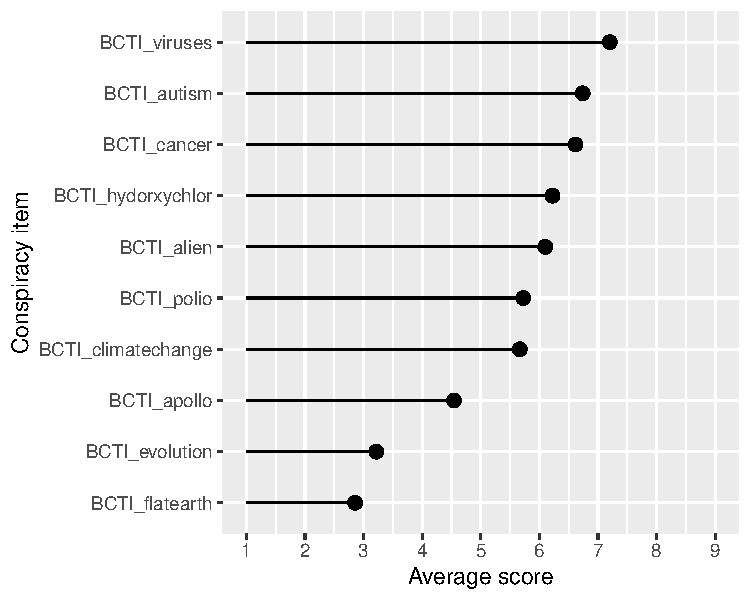
\includegraphics{output/figures/exp3-conspiracy-items.pdf}
\caption{\label{fig:exp3-conspiracy-items}Distribution of conspiracy thinking by item.}
\end{figure}

\subsection{Reasons for consensus rejection}\label{reasons-for-consensus-rejection-1}

\subsubsection{All raw answers}\label{all-raw-answers-1}

\begin{longtable}[t]{>{}r>{}l>{\raggedright\arraybackslash}p{30em}}
\caption{\label{tab:exp3-reasons-rejection}Reasons for consensus rejection}\\
\toprule
id & question & answer\\
\midrule
5 & lasers & It is what I believed I was taught\\
12 & antibiotics & I do not know\\
20 & water & I think I got it confused in my head. I was thinking 2 oxygen and 1 hydrogen.\\
25 & electrons & I made a mistake.\\
26 & antibiotics & I have always experienced receiving antibiotic for viral infections. So i do not agree that antibiotic does not kill viruses.\\
\addlinespace
32 & antibiotics & Because I realized that my thinking was not correct.\\
32 & orbit & After thinking about it, I realized  that it does take a year for the sun to go around the earth.\\
38 & continents & The earth is not millions of years old.\\
38 & orbit & The earth is flat and stationary.\\
43 & water & I got it confused. Its true. One oxygen and  2 hydrogen is what i learned in school.\\
\addlinespace
46 & sex & Yes.  Its normal to think that, however, not always.\\
53 & continents & The Earth was created aged by God and has not been around for millions of years. I do not believe in evolution but rather creation based on the Word of God.\\
61 & continents & I do not believe that the universe is millions of years old\\
62 & continents & I do not believe the theory that the earth is that old.\\
65 & electrons & Because I would like to see more research on this matter.\\
\addlinespace
65 & antibiotics & Because I would like to see more research on this matter.\\
65 & continents & Because I would like to see more research on this matter.\\
65 & diamonds & Because I would like to see more research on this matter.\\
65 & water & Because I would like to see more research on this matter.\\
72 & lasers & That’s the truth\\
\addlinespace
72 & salt & I wasn’t sure\\
83 & continents & The Earth has only been around for 6-7 thousand years. As far as I know however, the Continents have been moving.\\
83 & water & thought it was "2 parts oxide, one hydrogen." I was of course wrong. I also miss clicked the wrong answer for how long it takes the Earth the revolve around the sun... I think.\\
87 & electrons & I believe atoms are the smallest particles.\\
87 & continents & On second thought, I agree.\\
\addlinespace
87 & diamonds & On second thought, I believe I agree.\\
87 & water & This does not fit according to my recollection.\\
92 & salt & I meant to agree, I did not know the answer.\\
96 & electrons & I don't think electrons are smaller, just because that is what we were taught in science\\
96 & continents & This is something we are taught academically in science, it may not be true\\
\addlinespace
98 & antibiotics & I think there are two different kinds of antibiotics. One type kills bacteria infections and the other type kills viral infections\\
99 & continents & I don't have a reason to believe Earth has been here for millions of years, so I don't agree with the consensus. Of course, I know I could be wrong.\\
102 & continents & This information is based in evolution which is a theory.\\
109 & continents & I partially agree that continents have moved due to plate tectonics. But I don't believe the Earth is as old as it mentions in the explanation, and is much younger. I also disagree with scientific consensus and there is really no such thing. Because with science, when you base things on evidence and then find new evidence, you have to change your theory. So there is really no such thing as consensus, there is data, facts and theories.\\
112 & antibiotics & No\\
\addlinespace
112 & speed & No\\
112 & salt & No\\
117 & antibiotics & Not really. I thought they killed virus' but maybe I am wrong. heh.\\
117 & sex & I thought both male and female decided the fate of the babies gender.\\
122 & antibiotics & antibotics only kill bacteria\\
\addlinespace
122 & lasers & I thought they light was a lot faster than sound waves\\
122 & salt & not sure\\
129 & continents & YES, I believe in a young earth.  I do not accept the tax supported theory of evolution.\\
130 & antibiotics & I was confused.\\
132 & continents & Continental drift is an unproven theory. I have seen no actual evidence for it. Flooding and receding of waters are more likely the cause of coastline changes throughout history.\\
\addlinespace
132 & orbit & There is no scientific evidence that the earth moves at all except for earthquakes. The sun is clearly moving around the earth in a daily circular pattern. The sun is much smaller and closer than we have been taught.\\
142 & salt & I thought it was made up of that.\\
143 & lasers & Lasers operate based on the principles of stimulated emission of electromagnetic radiation, typically light.\\
146 & antibiotics & Different knowledge and experience.\\
146 & sex & A mothers choice not the fathers choice because of religious beliefs.\\
\addlinespace
146 & diamonds & Gained through knowledge and skills.\\
150 & speed & To be honest, I did actually hear the concept that like travels fashion and sound so I’m not sure why I picked that answer.\\
151 & lasers & I accidentally clicked the other answer I'm not going to lie. As soon as I clicked it on accident I was like "Sh*t". I meant to choose the other answer on this one, I'm sorry.\\
151 & salt & I misunderstood this question. This one confused me the most even though it's right in front of me. Sorry.\\
155 & salt & error\\
\addlinespace
158 & lasers & No I did not know this question.\\
158 & salt & I knew this one and just blanked on the answer.\\
159 & sex & I thought I read it said in most cases women transmit an X chromosome, but now I'm not sure.\\
161 & antibiotics & I thought antibiotics kills every bit of poison.\\
166 & electrons & I'm not sure, I dont' understand it\\
\addlinespace
166 & water & I'm not sure, I dont' understand it\\
171 & diamonds & It just doesn't sit well with me.\\
172 & sex & I was wrong. I agree with scientific consensus.\\
173 & orbit & Yes the scientist now more than I do\\
178 & electrons & I was incorrect on this.\\
\addlinespace
191 & antibiotics & I could be wrong, but I thought they killed viruses as well.\\
191 & continents & I do not believe without a doubt the earth has been around for millions of years.\\
196 & sex & Answered incorrectly in error.  I agree with the scientific consensus.\\
197 & antibiotics & I’ve taken antibiotics numerous of times and although my sickness is usually cured, I always get a yeast infection as result. This always happens since the antibiotics kill the good and bad bacteria in the body.\\
197 & sex & I believe that God decides whether parents will be blessed with a boy or girl. It had nothing to do with genetics.\\
\addlinespace
197 & diamonds & This just doesn’t seem correct even after viewing the article from the university. I can’t explain why but I can’t justify it.\\
198 & diamonds & I just never heard of diamonds being made of carbon and it makes zero sense to me while thinking about it.\\
200 & continents & The earth is not old but young. Not billions or millions but thanks of years.\\
200 & orbit & One day because the sun is not taking a year to light up other parts of the earth.\\
\bottomrule
\end{longtable}

\subsection{Why do people accept the scientific consensus:}\label{why-do-people-accept-the-scientific-consensus}

\subsubsection{Participants who answered ``other''}\label{participants-who-answered-other}

\begin{longtable}[t]{>{}r>{\raggedright\arraybackslash}p{30em}}
\caption{\label{tab:exp3-other-reasons-acceptance}Reasons for consensus rejection}\\
\toprule
id & other\_reason\_agreement\\
\midrule
24 & some stuff I already knew, other stuff I don't care about like atoms and molecules\\
37 & I mostly agreed based on my personal knowledge.\\
62 & I have never seen compelling evidence to disprove the consensus.\\
89 & Because it is true.\\
101 & I can't say that I trust scientists on many things, but on most in this survey. However, while I believe the continents have moved around, I don't believe the earth is millions of years old, as I'm a Christian. Though God never notes exactly how old the earth is, so it could be millions of years old.\\
\addlinespace
102 & Agreed due to vague knowledge about the subject.\\
166 & I'm not sure, you cant trust any party\\
172 & Because i recall previously being taught that\\
182 & I agree because the explaination makes sense\\
188 & I don't trust scientists, but those are the current established 'facts'. Which, on the mundane side of things, are likely true.\\
\addlinespace
189 & I take nothing that anyone tells me at face value. Lots of studying and verifying accuracy of the things that I was taught my entire life.\\
195 & I mostly agree with the consensus because I don't have the equipment to independently test it myself and I also know scientists have proven those who don't have the so called equipment to know what they know. We can only observe what we observe at the moment, but there's more to what the scientists are observing and theorizing.\\
\bottomrule
\end{longtable}

\subsection{How did participants independently verifiy?}\label{how-did-participants-independently-verifiy}

\subsubsection{Participants who answered ``other''}\label{participants-who-answered-other-1}

\begin{longtable}[t]{>{}r>{\raggedright\arraybackslash}p{30em}}
\caption{\label{tab:exp3-independent-verification}Reasons for consensus rejection}\\
\toprule
id & reason\_followup\\
\midrule
5 & By trying to remember\\
10 & Curiosity and the internet\\
12 & Guessed\\
14 & I double-checked the information on Google by looking up various websites, I did go with my initial gut instincts in most cases however if it was wrong upon verifying it then I would change my answer\\
18 & Prior knowledge from a formal education\\
\addlinespace
19 & I can check several different sources on the internet and see if they have the same verifiable information.\\
21 & I use intuition.  I use common sense.\\
22 & I have read it before, and did some experiments in chemistry class.  I look for scientific consensus on everything.  On these long established principles, I could have selected both answers.  I believe sometimes scientists are bribed or exhibit bias depending on who is funding them and what answers the funding entity wants. COVID treatments were a big example of that.  Hospitals were paid to execute certain protocols and disallow others.\\
27 & Most of the questions, the consensus answer was the same as my answer. For the one or two questions where it was not, I looked at who their sources were for the answers, and decided whether I believed those sources and how unsure I was about my answer and made my decision from there.\\
31 & Through exposure to scientific experiments and research that prove the claims valid and can be repeated with the same results occurring.\\
\addlinespace
36 & There is evidence and a good amount of understand about these issues. There isn't as much understanding when it comes to things like vaccines.\\
38 & Through many sources, including my own common sense and a lifetime of research into these matters.\\
39 & I used the information that I have learned in school and in the past.\\
40 & Most things I knew already as some were common knowledge\\
41 & My gut instinct.\\
\addlinespace
42 & Most was knowledge I already knew, however if I were to find out or look up info, I would simply consult the internet\\
43 & I thought about what i was told in school.\\
44 & I checked reliable sources, and I knew most of them from learning this information in science class.\\
48 & some things are obvious and don't need verification\\
49 & Research on my own as opposed to jist blindly following what the media is told to tell me.\\
\addlinespace
56 & extensive research\\
58 & I verified it with what then knowledge I know\\
67 & I remember some of the stuff from school.\\
68 & I clicked on two out of three of the links for most statements that I was unsure about.\\
71 & I have a lot of people who do deep research that verified the info.\\
\addlinespace
77 & Just various amounts of research online. There have been times where simple questions were simply ignored or answered in a perplexing manner. Those types of answers always raise a flag.\\
81 & By  the knowledge I already had.\\
82 & Some of these questions I remember from high school. And I learned this in science. Therefore I do remember alot of these questions.\\
88 & I don't know\\
97 & Either I already knew the information or after reading the information I can to my conclusion\\
\addlinespace
98 & My wife has taken two different kinds of antibiotics, one for viral infections and one for bacterial infections\\
100 & I independently verified the information by doing a lot of research and comparing studies.\\
103 & I do my own research.\\
114 & I guess I haven't independently verified the information.\\
116 & wikipedia articles and google searches\\
\addlinespace
120 & The questions I got wrong were facts that I had simply forgotten. Once made aware of the correct answer, I remembered that it was in fact the correct answer.\\
122 & heard of it before\\
123 & I used the links provided and then googled the question if I was unsure\\
126 & It is an obvious pattern whenever these events happen that there is a coverup, you just have to research the track record\\
129 & I'm unsure of which question, you asked several.  it's a bit confusing. the vaccine question has been verified by personal treatment and independent studies that were banned on social platforms\\
\addlinespace
131 & I used the information and links given to verify it.\\
132 & I have been studying this information for many years. Real science is not consensus alone. Peer review is rigged and fraudulent. We are not being given the truth about many things and most "scientists" don't even know that they are wrong and refuse to reinvestigate the topics.\\
136 & Have an educational background in anthropology and took a lot of science courses. I trust scientists generally but not always the way the findings are relayed.\\
137 & My own research, we were lied to in school\\
144 & By looking through multiple sources on a given topic.\\
\addlinespace
152 & A lot of this I have already learned, but I can't personally verify it bc I can't run the tests.\\
154 & I have done several science experiments to prove a lot of these ideas.\\
156 & looking it up online from at least 2-3 sources\\
159 & Instead of taking what the mainstream talking point is and immediately accepting it, I like to do further research myself.\\
161 & I already knew of the information presented to me for years.\\
\addlinespace
163 & I googled it and read information from various sources.\\
164 & Many of these tidbits of information are taught as introduction to different subjects. I have either studied this or have used Google  Academic to verify.\\
178 & Some of the questions I've done my own research on, others I can see with my own eyes.\\
185 & most of the questions i already knew the answer to because i researched it a long time ago\\
186 & The information presented is basic knowledge we learn throughout ours lives. Light travels faster than sound. The fathers genes decide whether ba baby will be male or female. Diamonds are formed from carbon. Calcium carbonate is not sodium chloride. It takes the earth 365.2ish to orbit our sun. Yes, water is 2 hydrogen, 1 oxygen. And and electron is much smaller than an atom. All things we learn in school. Oh and lasers use light waves not sound waves.\\
\addlinespace
187 & For light traveling faster then sound it's obviously verifiable because you see lightning before you hear thunder, lasers are visible so obviously they are made of light not sound, the definition of water is H2O so if something isn't H2O then it isn't water.  The vast majority of the questions were extremely common sense if you think about them for any amount of time.\\
191 & I either realized I was wrong or it sounded logical in my mind.\\
200 & The Bible.\\
\bottomrule
\end{longtable}

\subsection{Additional plots}\label{additional-plots-2}



\begin{figure}
\centering
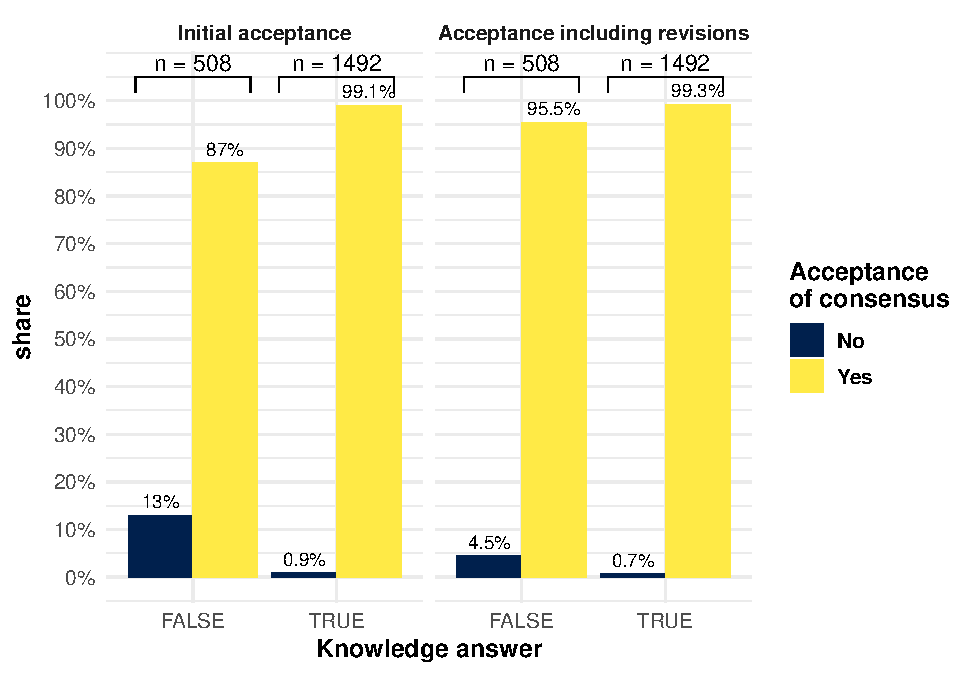
\includegraphics{output/figures/exp3-conditional-acceptance.pdf}
\caption{\label{fig:exp3-conditional-acceptance}Acceptance rates of scientific consensus, based on whether the initial response to the knowledge question was false or true.}
\end{figure}



\begin{figure}
\centering
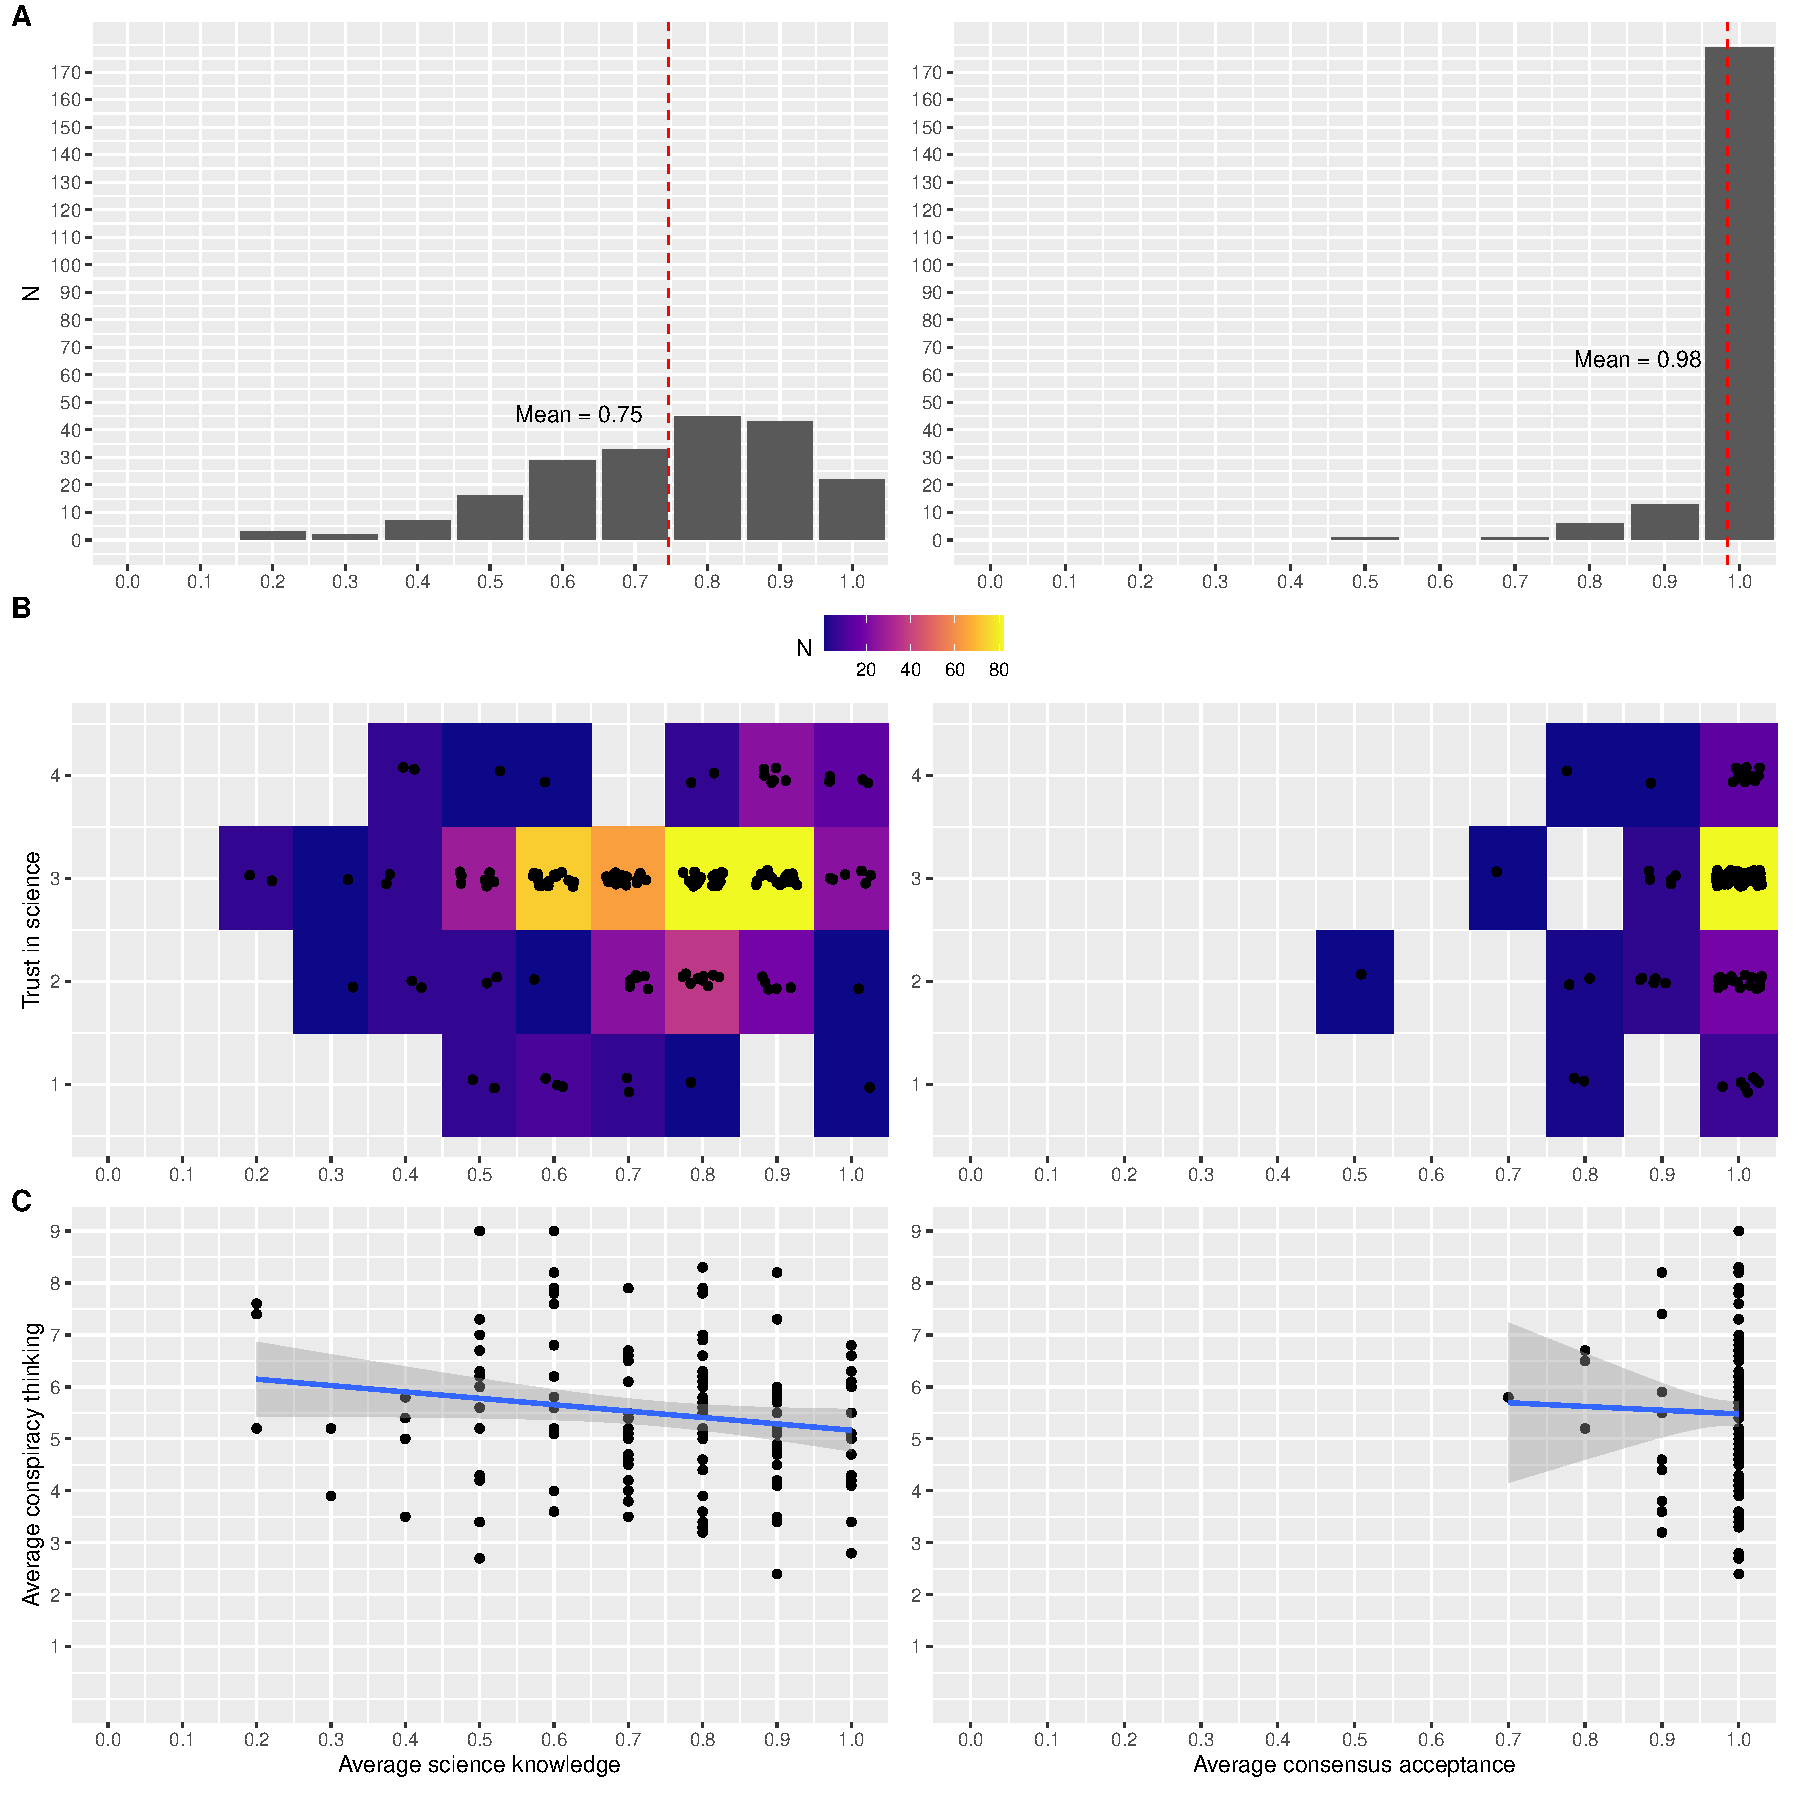
\includegraphics{output/figures/exp3-plot-overview.pdf}
\caption{\label{fig:exp3-plot-overview}\textbf{A} Shows the distribution of science knowledge (left) and acceptance of scientific consensus for participants who gave the wrong answer \textbf{B} Shows the relationship between trust in science and science knowledge/acceptance (if wrong at first, rounded to the first digit) of scientific consensus \textbf{C} Shows the relationship between conspiracy thinking and science knowledge/acceptance (if wrong at first) of scientific consensus}
\end{figure}

\clearpage

\section{Experiment 4}\label{exp4}

Study 4 relies on broadly the same design as study 3, and is again run on a sample of participants with vaccine-skeptic beliefs. The main difference is that study 4 uses a set of science questions which, instead of being on well-established facts, we are about more recent discoveries (Table \ref{tab:exp4-knowledge}). Our main question is whether participants will nevertheless readily accept the scientific consensus, as they did for the basic facts in previous studies.

As for the previous studies, we had the following hypotheses:

\textbf{H1a: Higher trust in science is associated with more science knowledge?}

\textbf{H1b: Higher trust in science is associated with more acceptance of the scientific consensus.}

\textbf{H2a: Higher conspiracy thinking is associated with less science knowledge?}

\textbf{H2b: Higher conspiracy thinking is associated with less acceptance of the scientific consensus.}

We had the following research questions:

\textbf{RQ1: What is the average science knowledge score?}

\textbf{RQ2: What is the average acceptance of the scientific consensus}

\textbf{RQ3: What reasons do participants provide to justify their rejection of the scientific consensus?}

\textbf{RQ4: In case they agree with the scientific consensus, do people feel that this is because of trust?}

\subsection{Participants}\label{participants-4}

We recruited a sample of participants holing vaccine-skeptic beliefs. Prolific Academic allows to filter out participants who have given specific answers to certain questions. We selected three available questions: 1. ``Participants were asked the following question: Please describe your attitudes towards the COVID-19 (Coronavirus) vaccines: {[}For (I feel positively about the vaccines); Against (I feel negatively about the vaccines); Neutral (I don't have strong opinions either way); Prefer not to say''{]}. We selected particpants who answered''Against''. 2. ``Participants were asked the following question: Have you received a coronavirus (COVID-19) vaccination? {[}Yes (at least one dose); No; Prefer not to answer{]}''. We select only people who answered ``No''. 3. ``Participants were asked the following question: On a scale from 1-7, please rate to what extent you agree with the following statement: I believe that scheduled immunizations are safe for children. {[}1 (TOTALLY DISAGREEE); 2 (DISAGREE); 3 (SOMEWHAT DISAGREE); 4 (NEITHER AGREE NOR DISAGREE); 5 (SOMEWHAT AGREE); 6 (AGREE); 7 (TOTALLY AGREE); Rather not say''{]}. We select only people who answered''1'', ``2'', or ``3''.

Based on these criteria, we recruited 200 participants from the US via prolific, of which two failed our attention check, resulting in a final sample of 198 participants (98 female, 100 male; \(age_\text{mean}\): 42.67, \(age_\text{sd}\): 12.32, \(age_\text{median}\): 41). Since we did not have any prior assumptions on effect sizes and our analyses were descriptive, we did not do a power analysis.

\subsection{Procedure}\label{procedure-3}

The procedure was identical to the one in experiment 3.

\subsection{Materials}\label{materials-5}

\FloatBarrier

Table \ref{tab:exp4-knowledge} shows all questions, their scientifically consensual answer, and their source. All but two questions were selected from existing science knowledge questionnaires. We tried to select non-political questions.

\begingroup\fontsize{8}{10}\selectfont

\begin{longtable}[t]{>{\raggedleft\arraybackslash}p{1em}>{\raggedright\arraybackslash}p{12em}>{\raggedright\arraybackslash}p{10em}>{\raggedright\arraybackslash}p{12em}}
\caption{\label{tab:exp4-knowledge}Science knowledge items}\\
\toprule
id & Question & Scientific consensus & Sources\\
\midrule
1 & For which disease is the drug bedaquiline, developed in 2007, a treatment? [Tetanus; Tuberculosis; Malaria] & There is a consensus among scientists that the drug bedaquiline is used against tubercolisis. & Sources: Wikipedia: https://en.wikipedia.org/wiki/Bedaquiline ;  Journal of applied microbiology: https://enviromicro-journals.onlinelibrary.wiley.com/doi/full/10.1111/jam.14478\#:\textasciitilde{}:text=The\%20drug\%20bedaquiline\%20was\%20approved,\%2DTB\%20and\%20XDR\%2DTB\\
2 & What is the maximum speed a proton can attain in the largest particle collider as to 2015? [90\% of the speed of light; 99\% of the speed of light; the speed of light] & There is a consensus among scientists that the maximum speed a proton can attain in the largest particle collider (the Large Hadron Collider) is 99\% of the speed of light. & Sources: Wikipedia: https://en.wikipedia.org/wiki/Large\_Hadron\_Collider\#Findings\_and\_discoveries ; CERN: https://home.cern/news/news/accelerators/first-successful-beam-record-energy-65-tev\\
3 & Kepler-452b is an exoplanet revolving around the star Kepler-452. How far away from the star is it, as established by astronomers in 2015? [97 million mi; 1,2 million mi; 1254 million mi] & There is a consensus among scientists that Kepler-452b is 97 million mi away from its star Kepler-452. & Wikipedia: https://en.wikipedia.org/wiki/Kepler-452b; NASA: https://science.nasa.gov/exoplanet-catalog/kepler-452-b/\\
4 & Using bomb-pusle dating with carbon 14, what is the age of the oldest known vertebrate, as established in 2016? [138 years; 205 years;  392 years] & There is a consensus among scientists that the oldest known vertebrate in 2016 was 392 years old, it is the Greenland shark. & Sources:  Wikipedia: https://en.wikipedia.org/wiki/Bomb\_pulse\#Applications Oxford University Research Archive: https://ora.ox.ac.uk/objects/uuid:6c040460-9519-4720-9669-9911bdd03b09\\
5 & How many more glials cells are there in the brain in comparison with neurons, as established in 2016? [The same amount; Twice as many; Tenth as many] & There is a consensus among scientists that there is the same amount of glial cells and neurons in the brain. & Sources: The Journal of Comparative neurology: https://onlinelibrary.wiley.com/doi/10.1002/cne.24040; Wikipedia: https://en.wikipedia.org/wiki/Glia\#Total\_number\\
\addlinespace
6 & As predicted by the general theory of relativity, how many times would the Earth keep orbiting if the Sun disappeared, as established in 2012? [47 seconds; 8 minutes;  2 hours] & There is a consensus among scientists that if the Sun disappeared, the Earth would keep orbiting for 8 minutes. & Sources: Wikipedia: https://en.wikipedia.org/wiki/Gravity\#Tests\_of\_general\_relativity ; Science Bulletin: https://link.springer.com/article/10.1007/s11434-012-5603-3\\
7 & What is the electric charge of the Higgs Boson, as established in 2012? [1.602176634 x 10-19; 0; 3.2x10-19C] & There is a consensus among scientists that the Higgs Boson does not have an electric charge, it is electrically neutral. & Sources: Wikipedia: https://en.wikipedia.org/wiki/Higgs\_boson\#cite\_ref-npr-interview\_189-0; Cern: https://home.cern/science/physics/higgs-boson\\
8 & What is the age of the oldest materials formed on Earth, as established in 2020? [Less than 4.6 Ga; Around 4.6 Ga; More than 4.6 Ga] & There is a consensus among scientists that the oldest materials formed on Earth are more than 4.6 Ga years old. & Sources: Wikipedia: https://en.wikipedia.org/wiki/Oldest\_dated\_rocks ; Proceedings of the National Academy of Sciences: https://www.pnas.org/doi/10.1073/pnas.1904573117\\
9 & With the best current cloning techniques, what is the average success rate when operated on mice, as of 2010? [2,7\%; 9,4\%; 17,2\%] & There is a consensus among scientists that the average success rate of the best current cloning techniques on mice is 9.4\%. & Sources: Wikipedia: https://en.wikipedia.org/wiki/Cloning\#cite\_note-112 ; Oxford Academic: https://academic.oup.com/biolreprod/article/83/6/929/2530195?login=false\\
10 & What was the strength of the Earth magnetic field 3.7 billion years ago, as discovered this year? [15 microtesla; 30 microtesla; 45 microtesla] & There is a consensus among scientists that the strength of Earth magnetic field 3.7 billion years ago was 15 microtesla. & Sources: Phys.org : https://phys.org/news/2024-04-oldest-undisputed-evidence-earth-magnetic.html; Science News: https://www.sci.news/othersciences/geoscience/earliest-evidence-earths-magnetic-field-greenland-12884.html\\
\bottomrule
\end{longtable}
\endgroup{}

\subsection{Results}\label{results-4}

By contrast to previous studies on basic science knowledge, participants on average answered only 36 \% (sd = 0.17) of the questions correctly (RQ1). Similar with previous studies, however, they initially accepted the scientific consensus on average for 86 \% (sd = 0.18) of the questions (RQ2). The acceptance rate is even higher when accounting for opinion revisions towards acceptance of the consensus, after initial rejection (91 \%, sd = 0.16).

Fig. \ref{fig:exp4-conditional-acceptance} illustrates the relationship between knowledge and acceptance. In most cases (83.7 \%), participants readily accepted the scientific consensus right after having given the wrong answer to a question. After providing the chance to revise the initial consensus rejection, this share is even larger (89.5 \%). In few (but still perhaps surprisingly many) cases (8.6 \%), participants who initially gave the correct response afterwards rejected the scientific consensus right after, thereby contradicting their own initial response. This share drops slightly after providing the chance to revise the initial consensus rejection (5.7 \%).

For all correlations, we include opinion revisions for measuring consensus acceptance. We find no statistically significant correlation between science knowledge and trust in science (r = 0.10, p = 0.144), but a small positive correlation between acceptance of scientific consensus and trust in science (r = 0.16, p = 0.029). Again, these findings might be partly due to ceiling effects: As illustrated in Fig. \ref{fig:exp4-plot}, (i) most people do trust science, and (ii) that is true even among people with low knowledge or acceptance rates. We do not find a statistically significant correlation between neither conspiracy thinking and science knowledge (r = -0.02, p = 0.742), nor between conspiracy thinking and acceptance of scientific consensus (r = -0.05, p = 0.498).

For RQ3, we got 255 answers from 95 different participants to the open-ended questions on why they had rejected the scientific consensus on a particular question. Table \ref{tab:exp4-justifications} summarizes these answers by five categories.

All answers can be read in the appendix.

\begin{table}[tbp]

\begin{center}
\begin{threeparttable}

\caption{\label{tab:exp4-justifications}Justifications by category}

\begin{tabular}{llll}
\toprule
Category & \multicolumn{1}{c}{N (instances)} & \multicolumn{1}{c}{Share (instances)} & \multicolumn{1}{c}{N (unique participants)}\\
\midrule
Not convinced & 146.00 & 57.3\% & 65.00\\
No justification & 78.00 & 30.6\% & 35.00\\
Religious Beliefs & 13.00 & 5.1\% & 8.00\\
Mistake & 12.00 & 4.7\% & 10.00\\
Personal convictions & 6.00 & 2.4\% & 4.00\\
\bottomrule
\end{tabular}

\end{threeparttable}
\end{center}

\end{table}

For RQ4, only 36.4\% of participants said they accepted the scientific consensus because they trust scientists on this question, while 47\% said they independently verified the fact. 16.7\% answered with other ``other'' and gave an open-ended explanation (see below for all open-ended answers).

We also asked all 93 participants who answered that they had independently verified the answer to explain how they did so. The open-ended answers are listed below.

\subsection{Comparing items}\label{comparing-items-3}

\subsubsection{Conspiracy theories}\label{conspiracy-theories-3}

Table \ref{tab:exp4-correlation-conspiracy} shows the correlations of the three different scales assessing conspiracy thinking.

\begin{table}[h]

\begin{center}
\begin{threeparttable}

\caption{\label{tab:exp4-correlation-conspiracy}Correlations of the three different scales assessing conspiracy thinking}

\begin{tabular}{llll}
\toprule
 & \multicolumn{1}{c}{BCTI} & \multicolumn{1}{c}{CMQ} & \multicolumn{1}{c}{SICBS}\\
\midrule
BCTI & 1.00 & 0.48 & 0.27\\
CMQ & 0.48 & 1.00 & 0.42\\
SICBS & 0.27 & 0.42 & 1.00\\
\bottomrule
\end{tabular}

\end{threeparttable}
\end{center}

\end{table}

\subsubsection{Trust in science}\label{trust-in-science-8}

Table \ref{tab:exp4-correlation-trust} shows the correlations of the three different items measuring trust in science.

\begin{table}[h]

\begin{center}
\begin{threeparttable}

\caption{\label{tab:exp4-correlation-trust}Correlations of the three different items measuring trust in science}

\begin{tabular}{llll}
\toprule
 & \multicolumn{1}{c}{wgm\_sciencegeneral} & \multicolumn{1}{c}{wgm\_scientists} & \multicolumn{1}{c}{pew}\\
\midrule
wgm\_sciencegeneral & 1.00 & 0.71 & 0.57\\
wgm\_scientists & 0.71 & 1.00 & 0.69\\
pew & 0.57 & 0.69 & 1.00\\
\bottomrule
\end{tabular}

\end{threeparttable}
\end{center}

\end{table}

\subsection{Correlations with alternative measures}\label{correlations-with-alternative-measures-3}

Table \ref{tab:exp4-correlations-outcomes} shows the correlations between knowledge and acceptance, respectively, and outcome variables.

\begin{table}[tbp]

\begin{center}
\begin{threeparttable}

\caption{\label{tab:exp4-correlations-outcomes}Correlations between knowledge and acceptance, respectively, and outcome variables}

\begin{tabular}{lll}
\toprule
outcome & \multicolumn{1}{c}{Correlation with knowledge} & \multicolumn{1}{c}{Correlation with acceptance}\\
\midrule
BCTI 
(main conspiracy measure) & -0.02 (p= 0.742) & -0.05 (p= 0.498)\\
CMQ & 0.11 (p= 0.112) & -0.1 (p= 0.156)\\
SICBS & 0.04 (p= 0.586) & -0.14 (p= 0.056)\\
WGM trust scientists & 0.14 (p= 0.045) & 0.26 (p< .001)\\
WGM trust general 
(main trust measure) & 0.1 (p= 0.144) & 0.16 (p= 0.029)\\
PEW trust scientists & 0.14 (p= 0.043) & 0.21 (p= 0.003)\\
\bottomrule
\end{tabular}

\end{threeparttable}
\end{center}

\end{table}

\subsection{Results conditional on false responses}\label{results-conditional-on-false-responses-3}

Table \ref{tab:exp4-false-response-regression} shows the correlations between acceptance and outcome variables based on linear regression models on standardized values.

\begin{table}

\caption{\label{tab:exp4-false-response-regression}Based on false response data only, correlations between acceptance and outcome variables based on linear regression models on standardized values}
\centering
\begin{tabular}[t]{lcccccc}
\toprule
  & BCTI\_avg & CMQ\_avg & SICBS & wgm\_scientists & wgm\_sciencegeneral & pew\\
\midrule
(Intercept) & 0.000 & 0.000 & 0.000 & 0.000 & 0.000 & 0.000\\
 & (0.071) & (0.071) & (0.070) & (0.069) & (0.070) & (0.070)\\
avg\_acceptance & -0.053 & -0.111 & -0.157* & 0.239*** & 0.148* & 0.186**\\
 & (0.071) & (0.071) & (0.071) & (0.069) & (0.071) & (0.070)\\
\midrule
Num.Obs. & 198 & 198 & 198 & 198 & 198 & 198\\
R2 & 0.003 & 0.012 & 0.025 & 0.057 & 0.022 & 0.035\\
R2 Adj. & -0.002 & 0.007 & 0.020 & 0.052 & 0.017 & 0.030\\
AIC & 566.3 & 564.4 & 561.9 & 555.2 & 562.5 & 559.9\\
BIC & 576.2 & 574.3 & 571.8 & 565.1 & 572.4 & 569.8\\
Log.Lik. & -280.165 & -279.212 & -277.970 & -274.621 & -278.246 & -276.951\\
RMSE & 1.00 & 0.99 & 0.99 & 0.97 & 0.99 & 0.98\\
\bottomrule
\multicolumn{7}{l}{\rule{0pt}{1em}+ p $<$ 0.1, * p $<$ 0.05, ** p $<$ 0.01, *** p $<$ 0.001}\\
\end{tabular}
\end{table}

\subsection{By-question variation}\label{by-question-variation-3}

\subsubsection{Knowledge}\label{knowledge-3}



\begin{figure}
\centering
\includegraphics{output/figures/exp4-questions-knowledge.pdf}
\caption{\label{fig:exp4-questions-knowledge}Distribution of correct answers by question.}
\end{figure}



\begin{figure}
\centering
\includegraphics{output/figures/exp4-questions-acceptance.pdf}
\caption{\label{fig:exp4-questions-acceptance}Distribution of consensus acceptance by question.}
\end{figure}

\subsection{Trust in science}\label{trust-in-science-9}



\begin{figure}
\centering
\includegraphics{output/figures/exp4-trust-scientists.pdf}
\caption{\label{fig:exp4-trust-scientists}Distribution of trust in scientists.}
\end{figure}

\subsection{Conspiracy thinking}\label{conspiracy-thinking-4}



\begin{figure}
\centering
\includegraphics{output/figures/exp4-conspiracy-distribution.pdf}
\caption{\label{fig:exp4-conspiracy-distribution}Distribution of conspiracy thinking.}
\end{figure}

\subsubsection{By-item variation}\label{by-item-variation-3}



\begin{figure}
\centering
\includegraphics{output/figures/exp4-conspiracy-items.pdf}
\caption{\label{fig:exp4-conspiracy-items}Distribution of conspiracy thinking by item.}
\end{figure}

\subsection{Reasons for consensus rejection}\label{reasons-for-consensus-rejection-2}

\subsubsection{All raw answers}\label{all-raw-answers-2}

\begin{longtable}[t]{>{}r>{}l>{\raggedright\arraybackslash}p{30em}}
\caption{\label{tab:exp4-reasons-rejection}Reasons for consensus rejection}\\
\toprule
id & question & answer\\
\midrule
5 & planet & I thought it was fake\\
6 & magnetic & I dont believe the earth has been here 3.7 billion years\\
10 & orbit & I honestly do not know anything about this stuff so i took a guess\\
10 & cloning & I took a guess\\
12 & material & seemed like too long of a time\\
\addlinespace
14 & cloning & I didn't think that many mice are actually cloned.\\
16 & orbit & I don't believe the Earth orbits the Sun.\\
16 & material & Nothing but their hypotheses without real evidence.\\
16 & magnetic & I'm not convinced the Earth existed 3.7 billion years ago.\\
23 & vertebrate & I don't believe in this kind of carbon dating. We can only slightly estimate the age, therefore I highly doubt the exact number of 392 years is accurate.\\
\addlinespace
23 & material & Earth is not billions of years old. At most, maybe 10,000 years. There is absolutely no way anything on Earth is billions of years old.\\
23 & magnetic & There was no magnetic field 3.7 billion years ago because the Earth was formed only around 6,000-10,000 years ago.\\
24 & cloning & I think it's less than that percentage\\
26 & vertebrate & no, just a guess\\
26 & brain & I have no idea.\\
\addlinespace
26 & material & No Idea\\
28 & material & I really could not explain this\\
28 & cloning & No, I could not explain this either\\
29 & orbit & Not enough science to prove.\\
29 & material & How can anyone put an  that age on something? Humans were not around the track.\\
\addlinespace
29 & cloning & Do not believe that anything can be cloned 100\%\\
32 & drug & Science is not always accurate.\\
32 & planet & N/A\\
32 & vertebrate & That doesn't seem accurate.\\
32 & brain & No.\\
\addlinespace
32 & boson & No.\\
32 & orbit & No.\\
32 & material & No.\\
32 & cloning & No.\\
32 & magnetic & No.\\
\addlinespace
35 & vertebrate & No, because I just guessed.\\
35 & orbit & No, I just guessed.\\
35 & material & No\\
41 & planet & i guessed\\
41 & vertebrate & i guessed\\
\addlinespace
41 & boson & i guessed\\
41 & magnetic & i guessed\\
42 & brain & There was a difference between what wiki said and the other article.\\
43 & vertebrate & I did not see anything to support this answer.\\
43 & brain & I did not feel like this was the correct answer.\\
\addlinespace
43 & material & Based on the article, I did not see this stated.\\
43 & cloning & There was nothing stated to prove this.\\
44 & vertebrate & I don’t see how it is possible to know the oldest vertebrate when there are so many species out there undiscovered\\
44 & brain & I don’t think I can explain it differently because I’m not an expert in science\\
44 & orbit & I am unsure if I can explain it differently, but how would we know if it never happened?\\
\addlinespace
44 & cloning & Again, this is a very detailed scientific question. I feel it so I will have to have extensive knowledge to answer this or I would have to have done an experiment on my own to to know this.\\
45 & drug & I am sure I heard it was used for malaria.\\
45 & cloning & I am not sure cloning is a definite technique.\\
49 & material & Religious reasons.\\
49 & magnetic & Religious reasons.\\
\addlinespace
54 & vertebrate & did not know the answer\\
54 & brain & did not know the answer\\
58 & cloning & The success rate just seems too high.\\
59 & vertebrate & The websites I read, seemed to have disagreed, unless I may have misread what I was fact checking.\\
60 & vertebrate & No.\\
\addlinespace
60 & orbit & No.\\
63 & planet & I don't know, but in my opinion when you are talking distance from star that is unknowable.\\
63 & vertebrate & I was guessing.  But knowing age via carbon dating is just guessing as well\\
63 & brain & I was guessing.  Same answer as others.\\
63 & boson & I was guessing.  But same answer.  They pretend to know things that are unknowable.\\
\addlinespace
63 & orbit & I was guessing.  Same answer as others.  Unknowable\\
63 & material & I was guessing.  This again is something unknowable.\\
63 & speed & I was guessing.  This is unknowable.\\
63 & magnetic & I was guessing.  This is unknowable.\\
65 & vertebrate & I couldn’t locate the proof\\
\addlinespace
65 & speed & The proof wasn’t clear to me\\
65 & cloning & Didn’t see the info to back this up\\
67 & material & Just a guess, I didn't think it made sense.\\
67 & speed & Figured it was the speed of light, turns out I was close.\\
68 & orbit & I'm not really able to give an explanation\\
\addlinespace
68 & speed & not really\\
68 & cloning & Not really\\
69 & orbit & It didn't make sense to me at the time.\\
69 & cloning & I thought it was easier to clone mice\\
70 & orbit & these were hypothesis on the ones i got wrong.\\
\addlinespace
70 & speed & it was a hypothesis, i had no idea\\
70 & magnetic & it was a hypothesis i had no clue\\
72 & drug & I do not believe in this consensus since it usually is fabricated\\
72 & vertebrate & This is usually fabricated\\
72 & brain & This is normally a fabricated fact\\
\addlinespace
72 & boson & This is probably fabricated\\
72 & orbit & I do not agree with nearly scientific fact since it is made up\\
72 & material & This is probably made up\\
72 & speed & I do think this consensus is faked\\
72 & magnetic & these are all made up terms\\
\addlinespace
74 & vertebrate & Because there was not evidence that I understood to support this theory.\\
74 & brain & Because the research that was provided does not fully support this theory.\\
74 & boson & Because the research that I read did not support our object this statement.\\
74 & orbit & The research that was credited does not give a direct amount of time just a formula to get the answer.\\
74 & material & I disagree with this statement because the research that was given says 4.6 GA years old not more than.\\
\addlinespace
74 & speed & I disagree because there are not enough facts to support this claim.\\
75 & orbit & Looking at the website given, I could not find the exact time of how long the Earth would keep orbiting, so I didn't agree.\\
75 & speed & I could not find the answer to that in the given websites\\
75 & cloning & I could not find data that supported that percentage.\\
78 & material & No, Just a thought.\\
\addlinespace
78 & cloning & Just a random thought\\
79 & orbit & N/A\\
80 & vertebrate & I actually meant to press agree after reading the wikipedia , it had mentioned how the oldest 'recorded' vertebrate was 392 years old\\
81 & drug & Malaria sounds more like the answer to this question, since it was developed more recently.\\
81 & brain & This question I have no idea. But I would be willing to answer differently if needed.\\
\addlinespace
81 & orbit & The Earth would still keep its orbit if the sun disappeared. I believe it would still take 365 days to do one full orbit on its axis.\\
83 & material & The Bible says the Earth is 6000 years old\\
84 & material & From a biblical perspective, this is not the case. Other than that, no.\\
87 & vertebrate & No, I was just guessing.\\
87 & speed & No. I was just guessing.\\
\addlinespace
88 & planet & God hasn't created stars that are millions of miles away from Earth or each other.\\
88 & orbit & God created the Earth as flat and stationary!\\
88 & material & God created the Earth 6,000 years ago.\\
88 & magnetic & God created the Earth 6,000 years ago.\\
92 & cloning & I feel that they've been cloning people with pretty great success for some time now.\\
\addlinespace
92 & magnetic & Because I don't agree that the earth is billions years old, since I'm a Christian.\\
93 & material & There is no way for man to know if it was actually formed on earth or if it was formed somewhere else and then ended up on earth.\\
94 & boson & I agree\\
94 & cloning & The articles I read were quite vague but all stated the success of cloning mice has been incredibly low, which made me disagree with the consensus\\
96 & orbit & I felt if the Sun disappeared than the Earth orbiting would be fast than 8 minutes.\\
\addlinespace
96 & speed & I would like to change my answer to agree.\\
96 & cloning & I would like to change my answer to agree.\\
97 & material & How do they know how old anything is?.  Everything we have been told by the powers that be for our whole lives has been a lie.  It is hard to believe anything anymore.\\
98 & speed & I was not able to find that information in the reference material.\\
98 & cloning & I was not able to find that answer in the reference material. And I guess I have a deep distrust of scientists, as well. Even if I read something that a scientist said on Wikipedia or Google I would not believe it. Remember it was the scientists who said safe and effective. And the Nazis have been cloning people since the 30s, so why believe anything they say about cloning mice.\\
\addlinespace
104 & vertebrate & It was just a guess.\\
104 & brain & It was just a guess.\\
104 & boson & It was just a guess.\\
104 & speed & It was just a guess.\\
105 & drug & I am unfamiliar.\\
\addlinespace
105 & orbit & Again I have no knowledge. It was a guess\\
106 & planet & Not sure I took a guess\\
106 & vertebrate & Not sure I took a guess\\
106 & brain & Not sure I took a guess\\
106 & material & Not sure I took a guess\\
\addlinespace
108 & material & I don’t trust the sources as anyone can make changes\\
113 & vertebrate & Because I dont think they really know themselves\\
113 & material & The earth has only been around a short time and it thousands not millions or billions of years\\
113 & magnetic & No dont believe the bible is the true map of mans existance and its not billions of years old\\
114 & planet & I tried to research it and didnt find the answer so i just chose anything\\
\addlinespace
114 & vertebrate & I just chose an answer because I didn't know\\
114 & material & I just chose anything because I didn't know the answer\\
114 & cloning & I just chose anything because I didn't know the answer\\
115 & vertebrate & It said the oldest known vertebrate was 252 years old\\
115 & speed & I didn’t see anywhere in the articles that backs this claim.\\
\addlinespace
118 & vertebrate & Aren't dinosaur bones older than 392 years old?\\
119 & material & If I understood the resources correctly I thought the time period was less. I'm questioning my answer now though!\\
121 & vertebrate & one of the articles i looked at said it was a smaller number I can't remember the number.\\
121 & material & I don't believe the earth is that old.\\
121 & cloning & I am not completely sure.  the number just seemed very large and I think that many of them die during the process.\\
\addlinespace
121 & magnetic & I'm not sure.  I still do not believe that the Earth is that old.\\
122 & speed & When reading the material that were given, I could not find the answer to confirm it. Therefore, since I could not confirm it, I did not accept the scientific consensus.\\
124 & planet & I didn't really understand the information on this one.\\
124 & boson & While reading the information provided I didn't see exact confirmation on if it has an electric charge or not.\\
124 & material & The answer was vague and not exact it just said more than 4 billion but not more than 4.6 billion.\\
\addlinespace
128 & drug & Because I thought it was the answer I had out.\\
128 & planet & It’s that far away.\\
128 & vertebrate & It shows that it was correct\\
128 & brain & Because of what I read.\\
128 & orbit & I had read it wrong.\\
\addlinespace
130 & brain & Neurons are everywhere.  I assumed that glials cells were not as prevalent as neurons.\\
130 & cloning & It was hard to believe science had progressed that much regarding cloning.  Cloning brings to mind science in the far future.\\
132 & orbit & I don't have anything scientifically to offer other than I just don't believe that's true.\\
133 & brain & I remember briefly coming across information on this subject and at the time they were thing they out numbered them 10.1. however that could of changed the more research that was done.\\
133 & cloning & i just assumed that cloning would not have a high success rate from reading about years ago, but I assume things have changed.\\
\addlinespace
134 & planet & I do not believe we can measure the distance of stars.\\
134 & orbit & I took a guess because I do not believe we can predict such a thing.\\
134 & material & I do not believe the earth is that old.\\
136 & cloning & I’m not sure that I believe that they are that successful.\\
137 & material & Not enough scientific proof\\
\addlinespace
137 & cloning & I don't believe in cloning techniques\\
137 & magnetic & It's possible that the earth magnetic field 3.7 billion years ago was 15 micro Tesla\\
139 & planet & I misread and thought they were talking about the distant from earth to Kepler.\\
139 & brain & It depends on the area of the brain and there could be some differences depending on which brains you are looking at.\\
139 & magnetic & I just wasn't sure.\\
\addlinespace
140 & vertebrate & No.\\
140 & brain & No\\
140 & material & No\\
140 & cloning & No\\
143 & planet & I don't trust that astronomers can accurately measure this.\\
\addlinespace
143 & vertebrate & I don't trust carbon 14 dating. I don't know what bomb-pusle is.\\
143 & orbit & I don't trust that scientists can estimate this accurately.\\
143 & material & I don't trust that scientists have a way to measure this accurately.\\
143 & magnetic & I don't trust that scientists have a way to measure this accurately.\\
145 & magnetic & i cant explain why i answered differently i probably forgot\\
\addlinespace
151 & boson & In some theoretical models or speculative physics, there might be hypotheses about different properties of the Higgs boson.\\
151 & speed & The exact percentage of the speed of light can vary slightly depending on the specific conditions and the state of the accelerator at any given time. Precision in reporting such values is crucial.\\
151 & cloning & The success rate might also depend on the specific strain of mice used or the conditions under which the cloning was performed. Variations in experimental conditions can affect the reported success rates.\\
152 & boson & Neutrality is a toxic line of thinking and only establishes constraints\\
152 & material & Universe is very old yes\\
\addlinespace
152 & speed & LHC is not what they say is it\\
152 & cloning & "sucess" for one thing but also this is vague and doesn't really say much\\
152 & magnetic & No way to really know this for sure and it also doesnt matter much\\
153 & orbit & I think if the sun disappeared the gravitational field would disappear nearly immediately; and the Earth would continue on in a straight line.\\
154 & orbit & I accept the scientific consensus but I do not accept Wikipedia as a confirming source of scientific data.\\
\addlinespace
154 & material & I don't have an explanation as to why I answered differently.\\
154 & speed & I thought from memory of my previous reading that my answer was correct.\\
155 & planet & I believe that there is not a way to accurately measure such a thing\\
155 & vertebrate & I believe that a lot of scientists make up numbers and the numbers aren't even accurate\\
155 & brain & This one might be accurate but I just wanted to disagree because I feel like it might not be accurate\\
\addlinespace
155 & orbit & I believe that a lot of those things about the Earth orbiting and stuff like that are misunderstood and not true\\
155 & material & I believe that the Earth is much younger than we're told and that allow those numbers about the Earth being trillions and trillions of years old is just crazy talk\\
155 & magnetic & I believe that the Earth does not have a magnetic field that's just a theory that is wrong in my opinion\\
157 & orbit & Sure, it's a prediction and one that doesn't sound very plausible to me.\\
157 & material & I don't believe the earth is that old.\\
\addlinespace
157 & magnetic & Once again, I don't believe the earth is that old.\\
159 & planet & Couldn't havesais it better myself\\
159 & material & No\\
163 & cloning & Because one of the links said 8 out of 10 success rate on cloning mice.\\
163 & magnetic & Because i didn't see anything showing that the researcher pulled samples from the northern most region to do the dating. There had been 2 other heating events that could have corrupted the data if they took it from the southern area.\\
\addlinespace
164 & orbit & I don't fully trust the sources and the Sun's never disappeared so how would they know.\\
167 & material & They are just guessing. There is no way to verify their estimates.\\
167 & magnetic & Earth age estimates are just guesses there is no way to verify them.\\
168 & planet & Scientific "Consensus" has low credibility in my perception.\\
168 & brain & Scientific "Consensus" has low credibility in my perception.\\
\addlinespace
168 & boson & Scientific "Consensus" has low credibility in my perception.\\
168 & orbit & Scientific "Consensus" has low credibility in my perception.\\
168 & material & Scientific "Consensus" has low credibility in my perception.\\
168 & speed & Scientific "Consensus" has low credibility in my perception.\\
168 & cloning & Scientific "Consensus" has low credibility in my perception.\\
\addlinespace
168 & magnetic & Scientific "Consensus" has low credibility in my perception.\\
169 & material & I don't think has to be that old.\\
171 & vertebrate & It did not sound right to me, and that science can be wrong too.\\
171 & cloning & I will agree with science on this one because they  create weird things.\\
172 & speed & I thought the article showed a different answer, but I looked back and read it again and confirmed the original statement is in fact true\\
\addlinespace
172 & cloning & I thought the article showed a different answer, but I looked back and read it again and confirmed the original statement is in fact true\\
173 & vertebrate & I think an older one has been found since 2016.\\
173 & brain & I think it is more likely there is a differing amount which may be very small but I really have no idea. I just know we humans are highly fallible and fallen and are wrong about things all the time.\\
173 & material & The Earth is no where near this old, it is around 6000-7000 years old. I cannot wait until we come to realize how utterly foolish we are in believing in the millions-billions or years old myth.\\
173 & magnetic & Same reason as above.\\
\addlinespace
174 & boson & The website was not convincing\\
174 & orbit & I thought it would be longer\\
175 & material & My final authority is the Bible.  It only goes back 6500 years to the creation.\\
175 & cloning & I just dont believe cloning techniques are that good my researched showed its around 1-2\%.\\
175 & magnetic & Earth was created around 6500 years ago.\\
\addlinespace
177 & material & I am a creationist and believe the earth is much younger than that and am not convinced the testing methods are correct\\
177 & cloning & number just seemed too high\\
181 & brain & There is a similar amount, but not the same amount.\\
181 & orbit & It's impossible to state as fact.\\
181 & material & It's impossible to state as fact.\\
\addlinespace
181 & magnetic & It's impossible to state as fact.\\
183 & planet & i read the distance in kilometers instead of miles.\\
183 & magnetic & i read that during this time the microteslas was 30-50\\
184 & vertebrate & Knowing how long vertebrates live today it seems unlikely that they lived significantly longer in the past\\
184 & material & There is so much variation when it comes to measuring the early days of earth that I would assume given enough time this estimate will change dramatically in the future\\
\addlinespace
188 & vertebrate & No I am not able to explain my answer.\\
188 & orbit & No.\\
192 & vertebrate & Based on what I read it’s not true.\\
192 & material & Based on what I read it’s not true.\\
192 & speed & I’m not sure if it’s true because I couldn’t find the proof for the claim in the material.\\
\addlinespace
192 & cloning & I don’t know if it is true because I couldn’t find the proof in the material.\\
194 & planet & It how I was taught.\\
194 & boson & I don't know\\
195 & planet & im a flat earther and i believe all the stars are right in our own atmosphere\\
195 & orbit & i dont believe that the earth orbits around the sun at all to be honest i think the sun and moon travel over the earth\\
\addlinespace
195 & material & i dont believe that the earth is that old\\
195 & magnetic & dont believe the earth is that old\\
197 & orbit & I could not find the reference to corroborate the information.\\
197 & material & The oldest material I found was just over 4.4 Ga\\
197 & speed & I could not find the reference to corroborate the information.\\
\bottomrule
\end{longtable}

\subsection{Why do people accept the scientific consensus:}\label{why-do-people-accept-the-scientific-consensus-1}

\subsubsection{Participants who answered ``other''}\label{participants-who-answered-other-2}

\begin{longtable}[t]{>{}r>{\raggedright\arraybackslash}p{30em}}
\caption{\label{tab:exp4-other-reasons-acceptance}Reasons for consensus rejection}\\
\toprule
id & other\_reason\_agreement\\
\midrule
8 & I didn’t know the answers at all so they could have been either one.\\
12 & questions were out of my realm and I had no interest in researching it\\
15 & I am not privy to information in he scientific field. I believe it to mostly be factual, but I'm unsure about discrepancies so I have to assume it may be true.\\
20 & I agreed with certain things because it's just how I felt.\\
23 & I didn't verify anything, nor do I really trust scientists, I guess I just believe that it's generally possible and seems like a reasonable calculation.\\
\addlinespace
25 & Not sure\\
26 & I wasn't sure either way.\\
35 & Neither, because I would have to do my own research beyond the untrustworthy sources you provided.\\
39 & I mostly agree because I obtained information from opposing sources and formed an opinion.\\
46 & I guessed\\
\addlinespace
63 & I haven't been able to independently verify it.  But I could if I wanted to and that information was something we could accurately figure out and prove it.\\
85 & I mostly agree with the consensus because they weren't politically-charged topics, and also, I've been able to independently verify the statements.\\
90 & There is no way for normal people to verify claims made by scientists with access to vast resources\\
92 & Seemed to be accurate\\
97 & I didn't really care what the answer was to those questions, so I just went with the flow.\\
\addlinespace
99 & I do not agree\\
104 & It was just a guess.\\
109 & i agreed with the consensus because i have not done my own research to refute it so what choice did i have. there’s not time enough on a survey for me to genuinely refute or agree so i mildly agree\\
110 & I chose that I didn’t\\
113 & I agree that things have been made and are scientifically real but not a billion or million years the bible does not confirm this and its smarter then science\\
\addlinespace
130 & I trust honest and ethical scientists.  The challenge is to find out who they are.  Science is an extraordinary discipline.  It should never be used to deceive and control us.\\
132 & A combination of both as I didn't check all of them but the ones that I did in deed checked out.\\
143 & I didn't have a reason to disagree with it.\\
152 & ALmost everything is subjective and "science" is wrong again and again although some things are objectively true with empirical evidence like math and 2 + 2 = 4\\
157 & I believe some of the questions are easier to verify than others.\\
\addlinespace
158 & I don't trust them that much because they are bought and paid for.\\
162 & I agreed because of my trust in scientists.\\
168 & I would agree if the subject involved could be independently verified, independent as in a non-aligned individual with any interests involving it.\\
173 & A mix of both, it largely depends on the subject matter. I will say I do not have a whole lot of trust in scientists as they are by and large secular in their views which distorts them a tremendous amount.\\
175 & The points I can agree with make sense and dont go against the Word of God.\\
\addlinespace
187 & I agreed because of my own research and knowledge coincides with the consensus.\\
189 & Agreed because I didn’t want to verify the information.\\
\bottomrule
\end{longtable}

\subsection{How did participants independently verifiy?}\label{how-did-participants-independently-verifiy-1}

\subsubsection{Participants who answered ``other''}\label{participants-who-answered-other-3}

\begin{longtable}[t]{>{}r>{\raggedright\arraybackslash}p{30em}}
\caption{\label{tab:exp4-independent-verification}Reasons for consensus rejection}\\
\toprule
id & reason\_followup\\
\midrule
2 & Online ,Google, youtube\\
3 & From the source and knowledge\\
5 & I compared the articles and their sources for accuracy\\
6 & Through research or facts I obtained previously\\
11 & Through the links provided or a google search. Some of these things I've heard in passing on TV or the radio\\
\addlinespace
17 & its just information i have researched over the years. One example would be aliens. The US government denied aliens being real for years but a couple years ago they told the public they are in fact real.\\
19 & I have not yet but will through factcheck.org.\\
21 & Reading links and googling more articles\\
24 & I have a friend and also Google.  I'm interested in scientific facts\\
27 & After I was showed the answer, I copied and pasted in into search bar and looked at other sources.\\
\addlinespace
31 & I researched it on a fact checked website\\
33 & I looked up each question. I have to just trust it at some point to answer the survey, but there are some things I'm not going to trust the internet for.\\
34 & I dif a lot of research on some of the questions..\\
36 & just an educated guess\\
37 & Through painstakingly tiring, wikipedia combing and years of just generally being inquisitive\\
\addlinespace
38 & Do my own research times ten\\
40 & I went to a couple of the provided links\\
41 & i did not\\
42 & By clicking on the links provided and reading the information.\\
43 & I searched multiple sites.\\
\addlinespace
44 & I would have to conduct experiments sent independently, verify it or read trustworthy sources\\
45 & Some of the information I have heard before.\\
48 & By finding additional sources\\
49 & My own research.\\
50 & I go and read multiple articles or studies\\
\addlinespace
51 & Through study and resources.\\
52 & I have done extensive research, read books from the library, watched DVDs and verified the information. After my mom died from a brain tumor I've researched the cures for cancer for 20 years now and know that doctors who come up with a cure are jailed or murdered to keep the status quo of the cancer industry. It's upsetting what our own government did in the 911 attacks on our own country as well.\\
56 & There were 2 links shown to confirm the answers.  The references were from scientists as well.\\
58 & There's lots of evidence.\\
59 & I only quickly checked. I have a hard time following Science, as it is not something I find interesting. However, I do like to fact check things when possible, and when provoked to do so.\\
\addlinespace
60 & I verified the information by clicking the links provided and using critical reasoning.\\
65 & Using the websites probided\\
67 & I always like to fact check stuff because I don't necessarily believe things at face value.\\
71 & I independently verified some of it a long time ago\\
72 & By lots of reading, research, and logic common sense\\
\addlinespace
74 & I read the documents that were given myself\\
75 & Read the provide websites to find agreeable information, also quick searches provided some verifications.\\
76 & Wikepedia\\
77 & I didn't\\
79 & I used google. Which I would say is an elementary resource for information, but it was good for answering such questions\\
\addlinespace
82 & Non- mainstream media sources, government documents, intuition.\\
83 & Research on my own\\
86 & I researched on google.\\
87 & By the websites you listed.\\
95 & I knew some things and from personal opinions\\
\addlinespace
98 & I use the Brave browser. Less censorship.\\
101 & I checked online with various sources to make sure they were true\\
102 & Checking the websites provided\\
107 & you need to add questions about where scientists get there funding from, and whether or not we would trust a statement like, all scientists agree\\
108 & I just went with my gut\\
\addlinespace
111 & I like to read a lot from all sorts of different sources, then read arguments that disagree with them. Eventually I'll find a grain of truth in all of that and use pattern recognition to fill in gaps based on what I know.\\
114 & Just did a google search\\
115 & I read the articles.\\
116 & Though previous knowledge and research\\
117 & I clicked the links to read what was stated.\\
\addlinespace
118 & I did a quick look on Google and searched on my own\\
119 & Google and the resources shown during the study\\
120 & I do my own research.\\
121 & i used the links in the study and looked briefly, at the articles.  Didn't understand most of it but made best decision I could.\\
122 & I read the material that was given within each of the questions and found the information.\\
\addlinespace
123 & I checked various sources and informational circles\\
124 & I searched up the information and researched myself.\\
126 & I looked at the websites cited in the questions.\\
127 & did web searches\\
133 & Well not exactly verified , but Just things I have researched or came across while online. there is a lot of information out there and a lot of misinformation. You just have to take a side\\
\addlinespace
135 & doing research and reading articles and scientific studies.\\
136 & By clicking the links provided\\
137 & I somewhat trust scientist but overall, I independently do my own research to verify such existing's\\
138 & Did much research and corroborated each finding or information and lined up against each other to see similar outcomes.\\
139 & By looking up the links to reputable sources and seeing if they match up with what other reputable sources are saying.\\
\addlinespace
140 & Verified persons in specialized authority.\\
141 & I just do my own research and look into things and how they could or couldn’t work\\
145 & i was informed  by trusted sources\\
147 & I checked the links given\\
154 & Online research of more trusted sources\\
\addlinespace
155 & Basically it aligns with other things I believe to be true so I will agree with it I'm not saying that I went out of my way and did a bunch of different studies but the thing about a lot of scientific research and studies if the foundation of the study is unstable or unreliable then I can't trust that a lot of the results are accurate\\
156 & I clicked on the articles and read for myself. Instead of trusting the information listed in the survey on its own I clicked the links to verify the information.\\
163 & i either knew the information or i followed the links provided and believed the information.\\
166 & I search multiple doctors and scientists and compare there work and theories\\
167 & I read research papers and look for inconsistencies or bad methodology.\\
\addlinespace
170 & Google search it\\
171 & I heard of these questions before, and I looked at the sources and my sources.\\
172 & I read the attached files to see if the info could be backed up on there as well. The 2 I thought I read as false I ended up doing a google search to confirm that the statements were in fact true\\
176 & I didn’t but I will\\
179 & I research various sources that lean in either direction (left or right) as well as sources that appear, at least on the surface, to be impartial. After gathering all of this information, I make my informed decision.\\
\addlinespace
183 & asking ai such as chatgpt\\
184 & Through my own research and comparison to other studies and others research.\\
188 & I looked it up using the links provided to me.\\
191 & By clicking and reading the link\\
192 & I read the articles and found the actual answer to the question.\\
\addlinespace
194 & Online\\
195 & google and research\\
197 & With the references provided in the study.\\
\bottomrule
\end{longtable}

\subsection{Additional plots}\label{additional-plots-3}



\begin{figure}
\centering
\includegraphics{output/figures/exp4-conditional-acceptance.pdf}
\caption{\label{fig:exp4-conditional-acceptance}Acceptance rates of scientific consensus, based on whether the initial response to the knowledge question was false or true.}
\end{figure}



\begin{figure}
\centering
\includegraphics{output/figures/exp4-plot-overview.pdf}
\caption{\label{fig:exp4-plot-overview}\textbf{A} Shows the distribution of science knowledge (left) and acceptance of scientific consensus for participants who gave the wrong answer \textbf{B} Shows the relationship between trust in science and science knowledge/acceptance (if wrong at first, rounded to the first digit) of scientific consensus \textbf{C} Shows the relationship between conspiracy thinking and science knowledge/acceptance (if wrong at first) of scientific consensus}
\end{figure}


\end{document}
